\chapter{Sample Preparation Procedures}

This appendix details the standardized sample preparation procedures used for the experiments in this dissertation. These techniques, if followed carefully, yield very repeatable results. Techniques for the double direct shear configuration for the biaxial apparatus and the low confining pressure triaxial jacket configuration are described.

\section{Biaxial Double Direct Shear}

Most of the experiments in this dissertation were completed using the double direct shear (DDS) geometry outside of the pressure vessel on the biaxial apparatus. This construction technique can easily be applied to solid block experiments in which blocks of rock take the place of the forcing blocks used and gouge is optional. This appendix will describe how to construct a granular DDS sample.

\subsection{Materials}
\begin{itemize}
\item (2) Side forcing blocks
\item (1) Center forcing block
\item (4) Side shields and screws
\item (2) Large steel blocks
\item (1) Cellophane tape
\item (1) New razor blade
\item (4) Jig blocks
\item (1) Set of spacing shims
\item (1) Steel rule
\item (1) Flat metal plate
\item (1) Rubber sheet
\item (1) Beaker or measuring cup
\item (1) Spoon
\item (1) Scissors
\item (1) Appropriate tool for side shield screws
\item (1) Wire brush set
\item (1) Large quick clamp
\item (1) Isopropyl alcohol
\item (1) Bulk granular material
\end{itemize}

\subsection{Procedure}
\begin{enumerate}
\item Thoroughly clean all forcing blocks and sample preparation surface with brushes and alcohol. Let air dry. \ref{Fig:dds_clean}
\item Setup one of the jig blocks at the rear of the sample preparation area. Find an appropriate combination of shims \ref{Fig:dds_thickness_blocks}to make the space measured from the side block (across the groove direction) to the top of the jig block the desired layer thickness \ref{Fig:dds_thickness_meas}.
\item Label the shim blocks, generally by making a unique set of permanent marker lines on the sides of the shims. This makes it easier to keep the shims together during your run of experiments.
\item Wrap a side block with a layer of cellophane tape. The tape should be about 3-5 mm back from the rough surface. Go around all four sides, using the dull back side of a razor blade to help hold the last corner square \ref{Fig:dds_wrap_trim}.
\item Trim the tape and ensure a clean seal around the block.
\item Wrap a second layer of tape around the side block, this time with the back of the tape flush with the smooth side of the block.
\item Trim the second layer of tape and check that the seal is solid \ref{Fig:dds_two_tape_layers}.
\item Lay the side block down onto the spacing shims and surround it with jig blocks. Use a small piece of tape to secure the jig blocks together \ref{Fig:dds_trim_setup}.
\item Use the razor blade to trim the tape sticking above the jig blocks \ref{Fig:dds_tape_trim}. Using a sub-parallel angle seems to work best. Use a new razor blade for each experiment to ensure a clean cut. If the tape tears anywhere, remove all tape, clean the block, and start again.
\item Repeat steps 4-9 for the second side block.
\item Label the side blocks with a permanent marker using a letter to indicate the material and a block designation. For example, ``SA" and ``SB" for steel , ``TA" and ``TB" for titanium blocks \ref{Fig:dds_blocks_labeled}.
\item Weigh each block and record the weight \ref{Fig:dds_block_weight}.
\item Dispense enough granular material to fill a side block into a beaker/cup and weigh the cup. Record this mass.
\item Place a side block back into the shim/jig block assembly and secure the jig blocks with tape.
\item Using the spoon, evenly distribute the granular material into the cavity of the side block \ref{Fig:dds_pour_material}.
\item Using the edge of a steel rule, wipe the material around until the block is covered to depth, adding material if necessary.
\item Using a pulling/cutting motion, make an even layer of material a few millimeters higher than the surface of the jig blocks \ref{Fig:dds_cutup_sample}.
\item Place the flat metal plate on top of the layer and press firmly. Using several CPR-like compressions to compact the material \ref{Fig:dds_press_sample}.
\item Pull the steel rule across the surface of the jig blocks to make a clean and level layer of granular material \ref{Fig:dds_level_sample}. Make sure any extra material goes back into the beaker/cup.
\item Repeat steps 15-19 a second time for the same side block.
\item Carefully untape the jig blocks and remove the side block. Using your palm, remove any material stuck to the outside surfaces of the block \ref{Fig:dds_finished_sideblock}.
\item Weigh the block and record its mass. From the two block mass measurements, calculate the weight of the granular material in the layer and record it. This should be very similar between each side block and each identical run. Differences of more than a few grams should be scrutinized and the layer possibly rebuilt.
\item Weigh the cup with the remaining granular material and determine the weight of the granular material used. This should be similar to, but generally more than, weighing the blocks due to material loss. This method is redundant for many experiments, but in 10 x 10 cm steel experiments, the weight of the loaded side blocks often exceed the maximum capacity of the lab balance and this method is necessary.
\item Repeat steps 13-23 for the second side block.
\item Using two large steel blocks and a quick clamp, build an ``L" shaped structure as a jig for assembling the sample \ref{Fig:dds_ell_jig}.
\item Using a steel rule, place the shims in the bend of the ``L" half of the sample width from each side so that they support the side block in its center.
\item Carefully place a side block on the shims with the mounting screw holes for the side shields facing you \ref{Fig:dds_sideblock_jig}. Take care to further orient the block if your blocks have special features such as holes for thermistors or other equipment.
\item Place a jig block across the end of the center block running in the front-back orientation \ref{Fig:dds_sideblock_jig_2}.
\item Place the center block in the corner of the ``L" jig (above the side block) with the long dimension running left-right.
\item Lower the center block onto the sample. Place a jig block on the far right end of the block to serve as a counter weight and reduce uneven force on the sample due to the unsupported end of the block \ref{Fig:dds_centerblock_jig}.
\item Unclamp the steel blocks and move the back block to the far right of the center block to serve as a backstop when taping the sample. Set the block on the left off to the side \ref{Fig:dds_move_block}.
\item Take an approximately 8" length of tape from the dispenser and pass it close to all edges of the sample. Static electricity will often pull away any loose material. If your sample is especially difficult (such as glass beads) this step can be omitted as long as you pass each strip of tape over a grounded object to remove the static charge.
\item Tape the three exposed sides of the sample with a single strip of tape centered on the layer \ref{Fig:dds_one_strip_tape}.
\item Re-tape this seam with two more strips, one slightly above the layer centerline and one slightly below \ref{Fig:dds_three_strip_tape}.
\item Carefully peel any tape that has stuck to the jig block and stand the sample up \ref{Fig:dds_standup_one_block}.
\item Using a razor blade, cut the tape running along the center block above the side block vertically and stick it over the top of the layer.
\item Using another piece of tape, completely seal the top of the layer \ref{Fig:dds_one_block_taped}.
\item Repeat steps 25-37 for the second side block. Lowering the sample assembly is more difficult due to the increased weight, but great care should be taken to ensure that it remains square in the jig \ref{Fig:dds_two_block_jig}.
\item Using a razor blade, trim out the holes for the side shield screws \ref{Fig:dds_trim_holes}.
\item Cut a strip of rubber sheeting and set the sample on it, centered in both directions.
\item Mark the location of the side shield holes and the side blocks on the sheet \ref{Fig:dds_mark_rubber}.
\item Cut the sheet so it is the width of the side shield hole spacing of the sample assembly.
\item Cut the corners of the sheet diagonally using the marks for the location of the center block edges \ref{Fig:dds_trimmed_rubber}.
\item Place the sample assembly onto the rubber sheet and tape the flaps to the center block \ref{Fig:dds_taped_rubber}.
\item Attach and tighten the side shields \ref{Fig:dds_side_shields}.
\item Measure the width of the sample using calipers and record this on the experimental log sheet \ref{Fig:dds_measure_sample}.
\item If the sample is not run immediately, store it between steel blocks \ref{Fig:dds_store_sample}.
\end{enumerate}

%% Figure %%
\begin{figure}
	\centering
        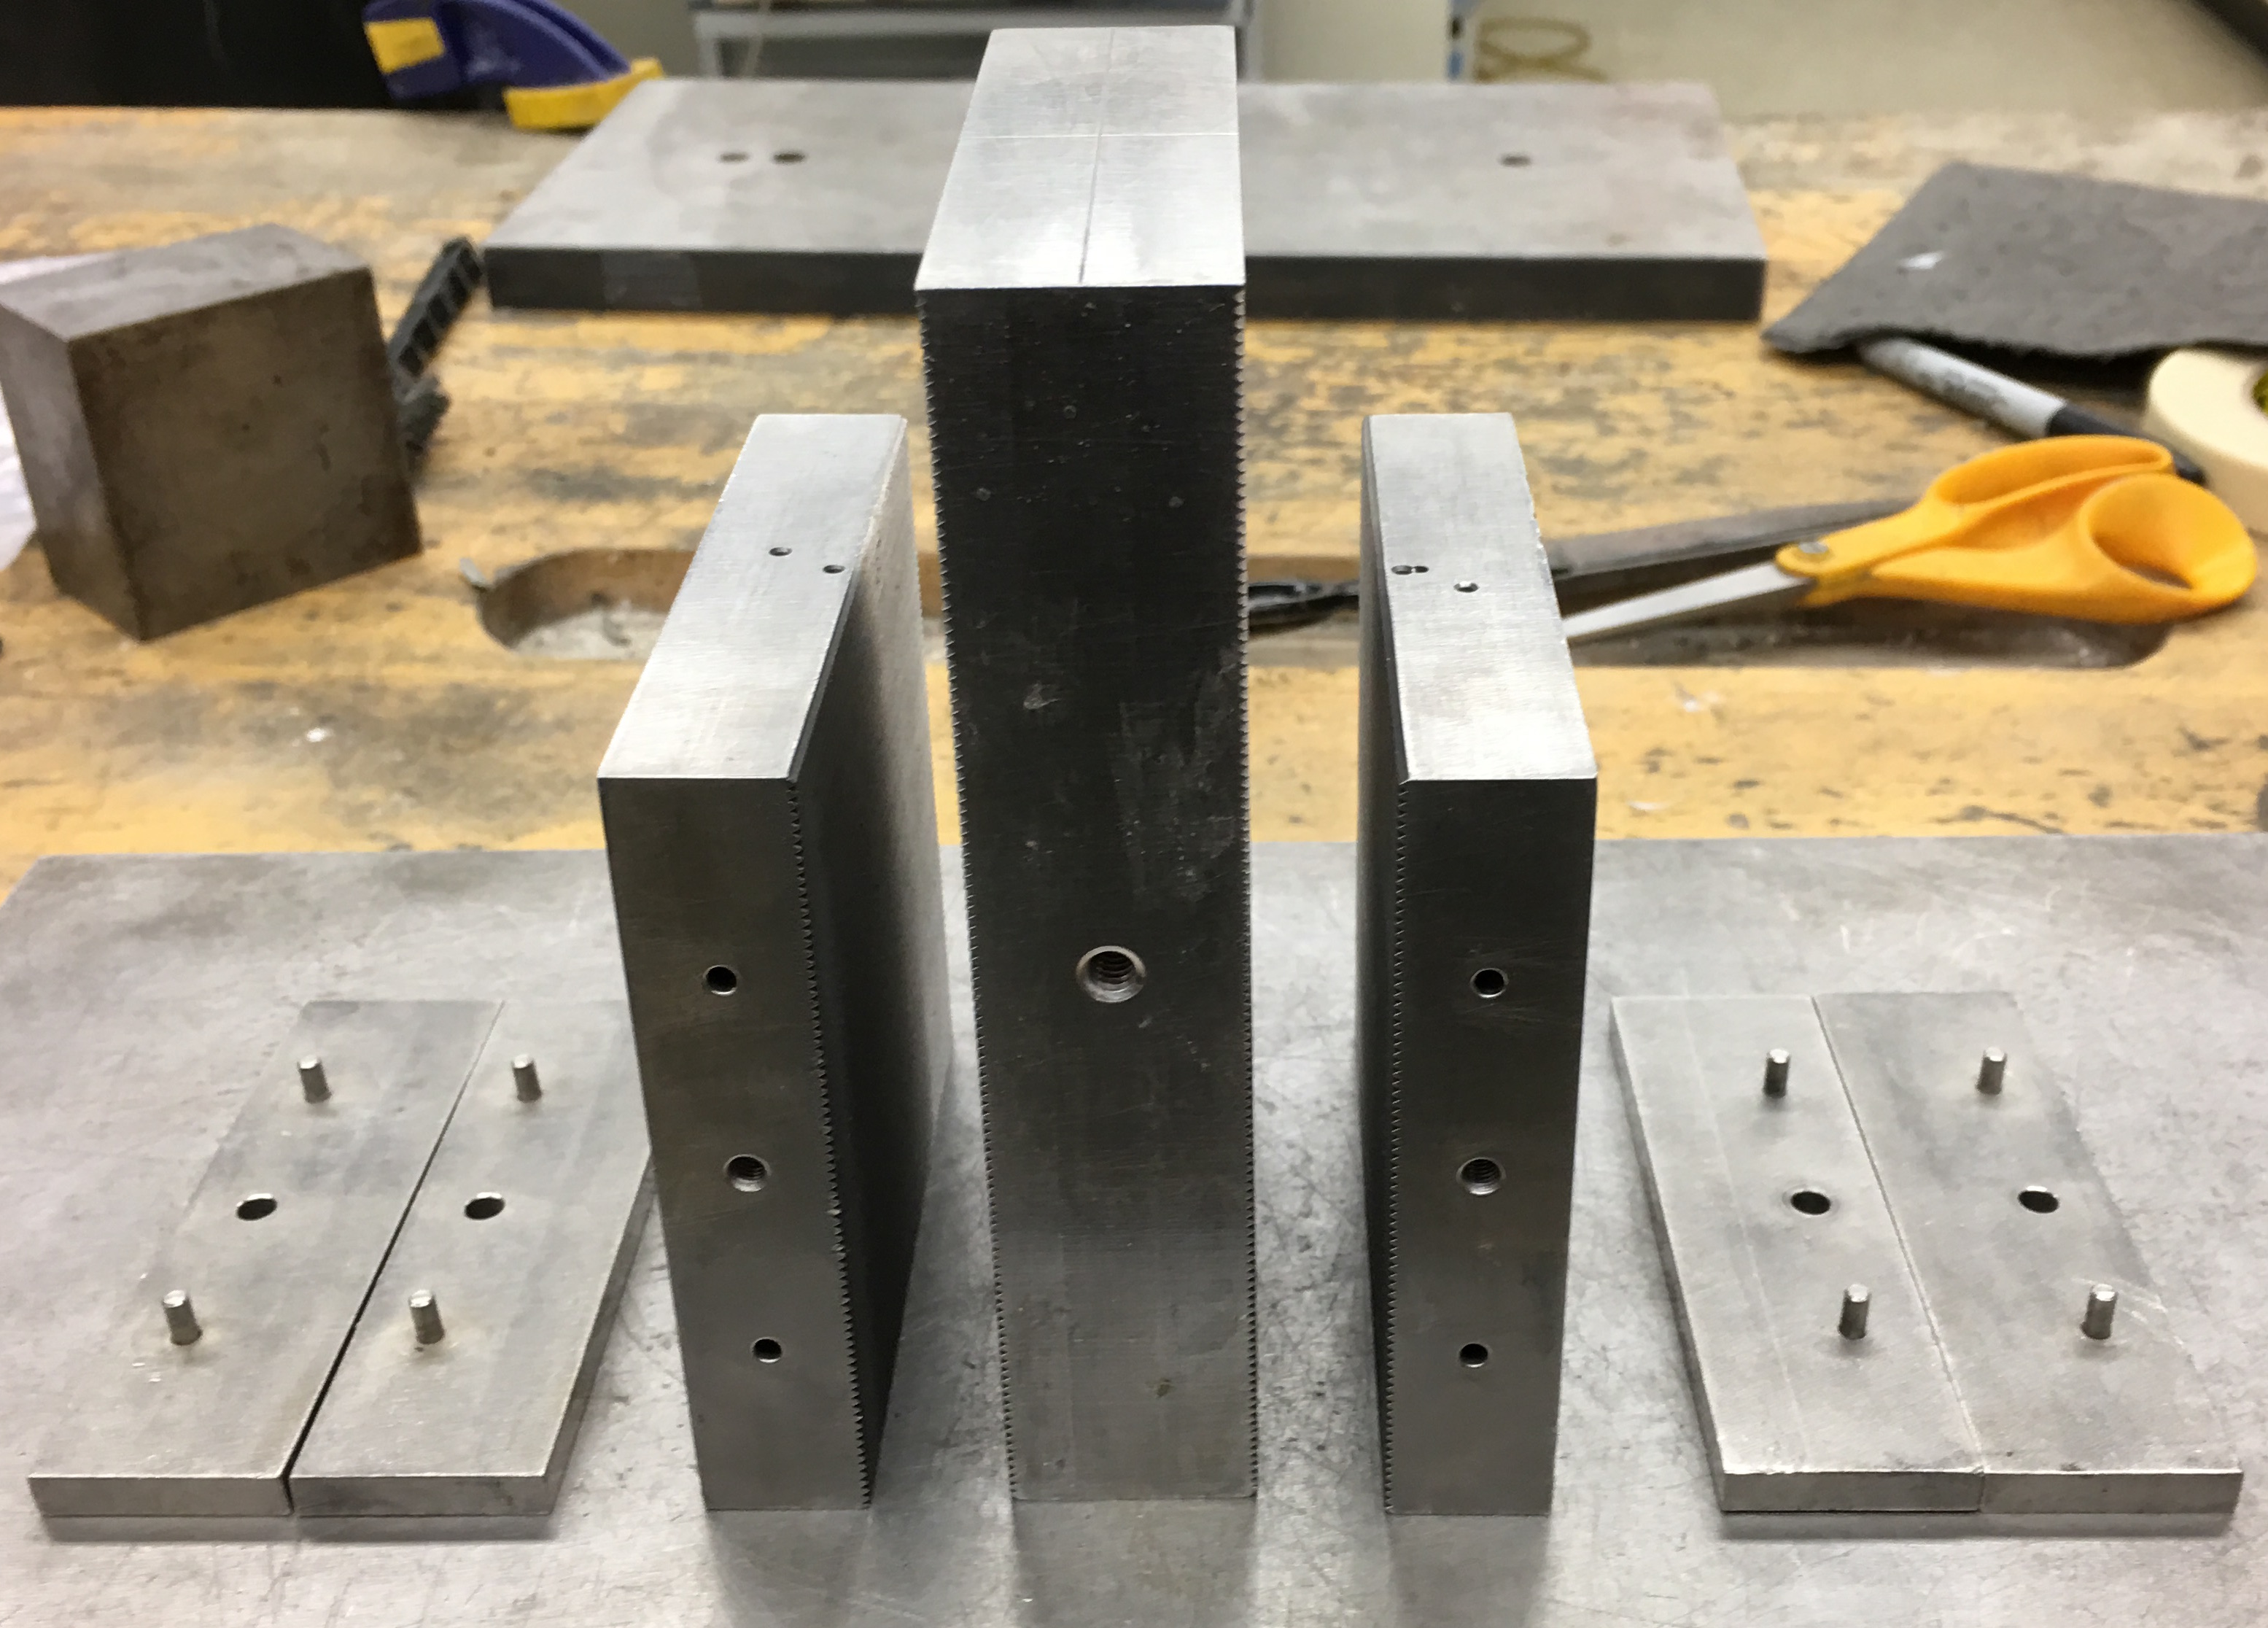
\includegraphics[width=0.7\textwidth]{appendix_sample_prep/dds_clean_blocks.jpg}
   	\caption{Gather all blocks and ensure that they are clean and free of debris.}
  	\label{Fig:dds_clean}
\end{figure}
%% End Figure %%

%% Figure %%
\begin{figure}
	\centering
        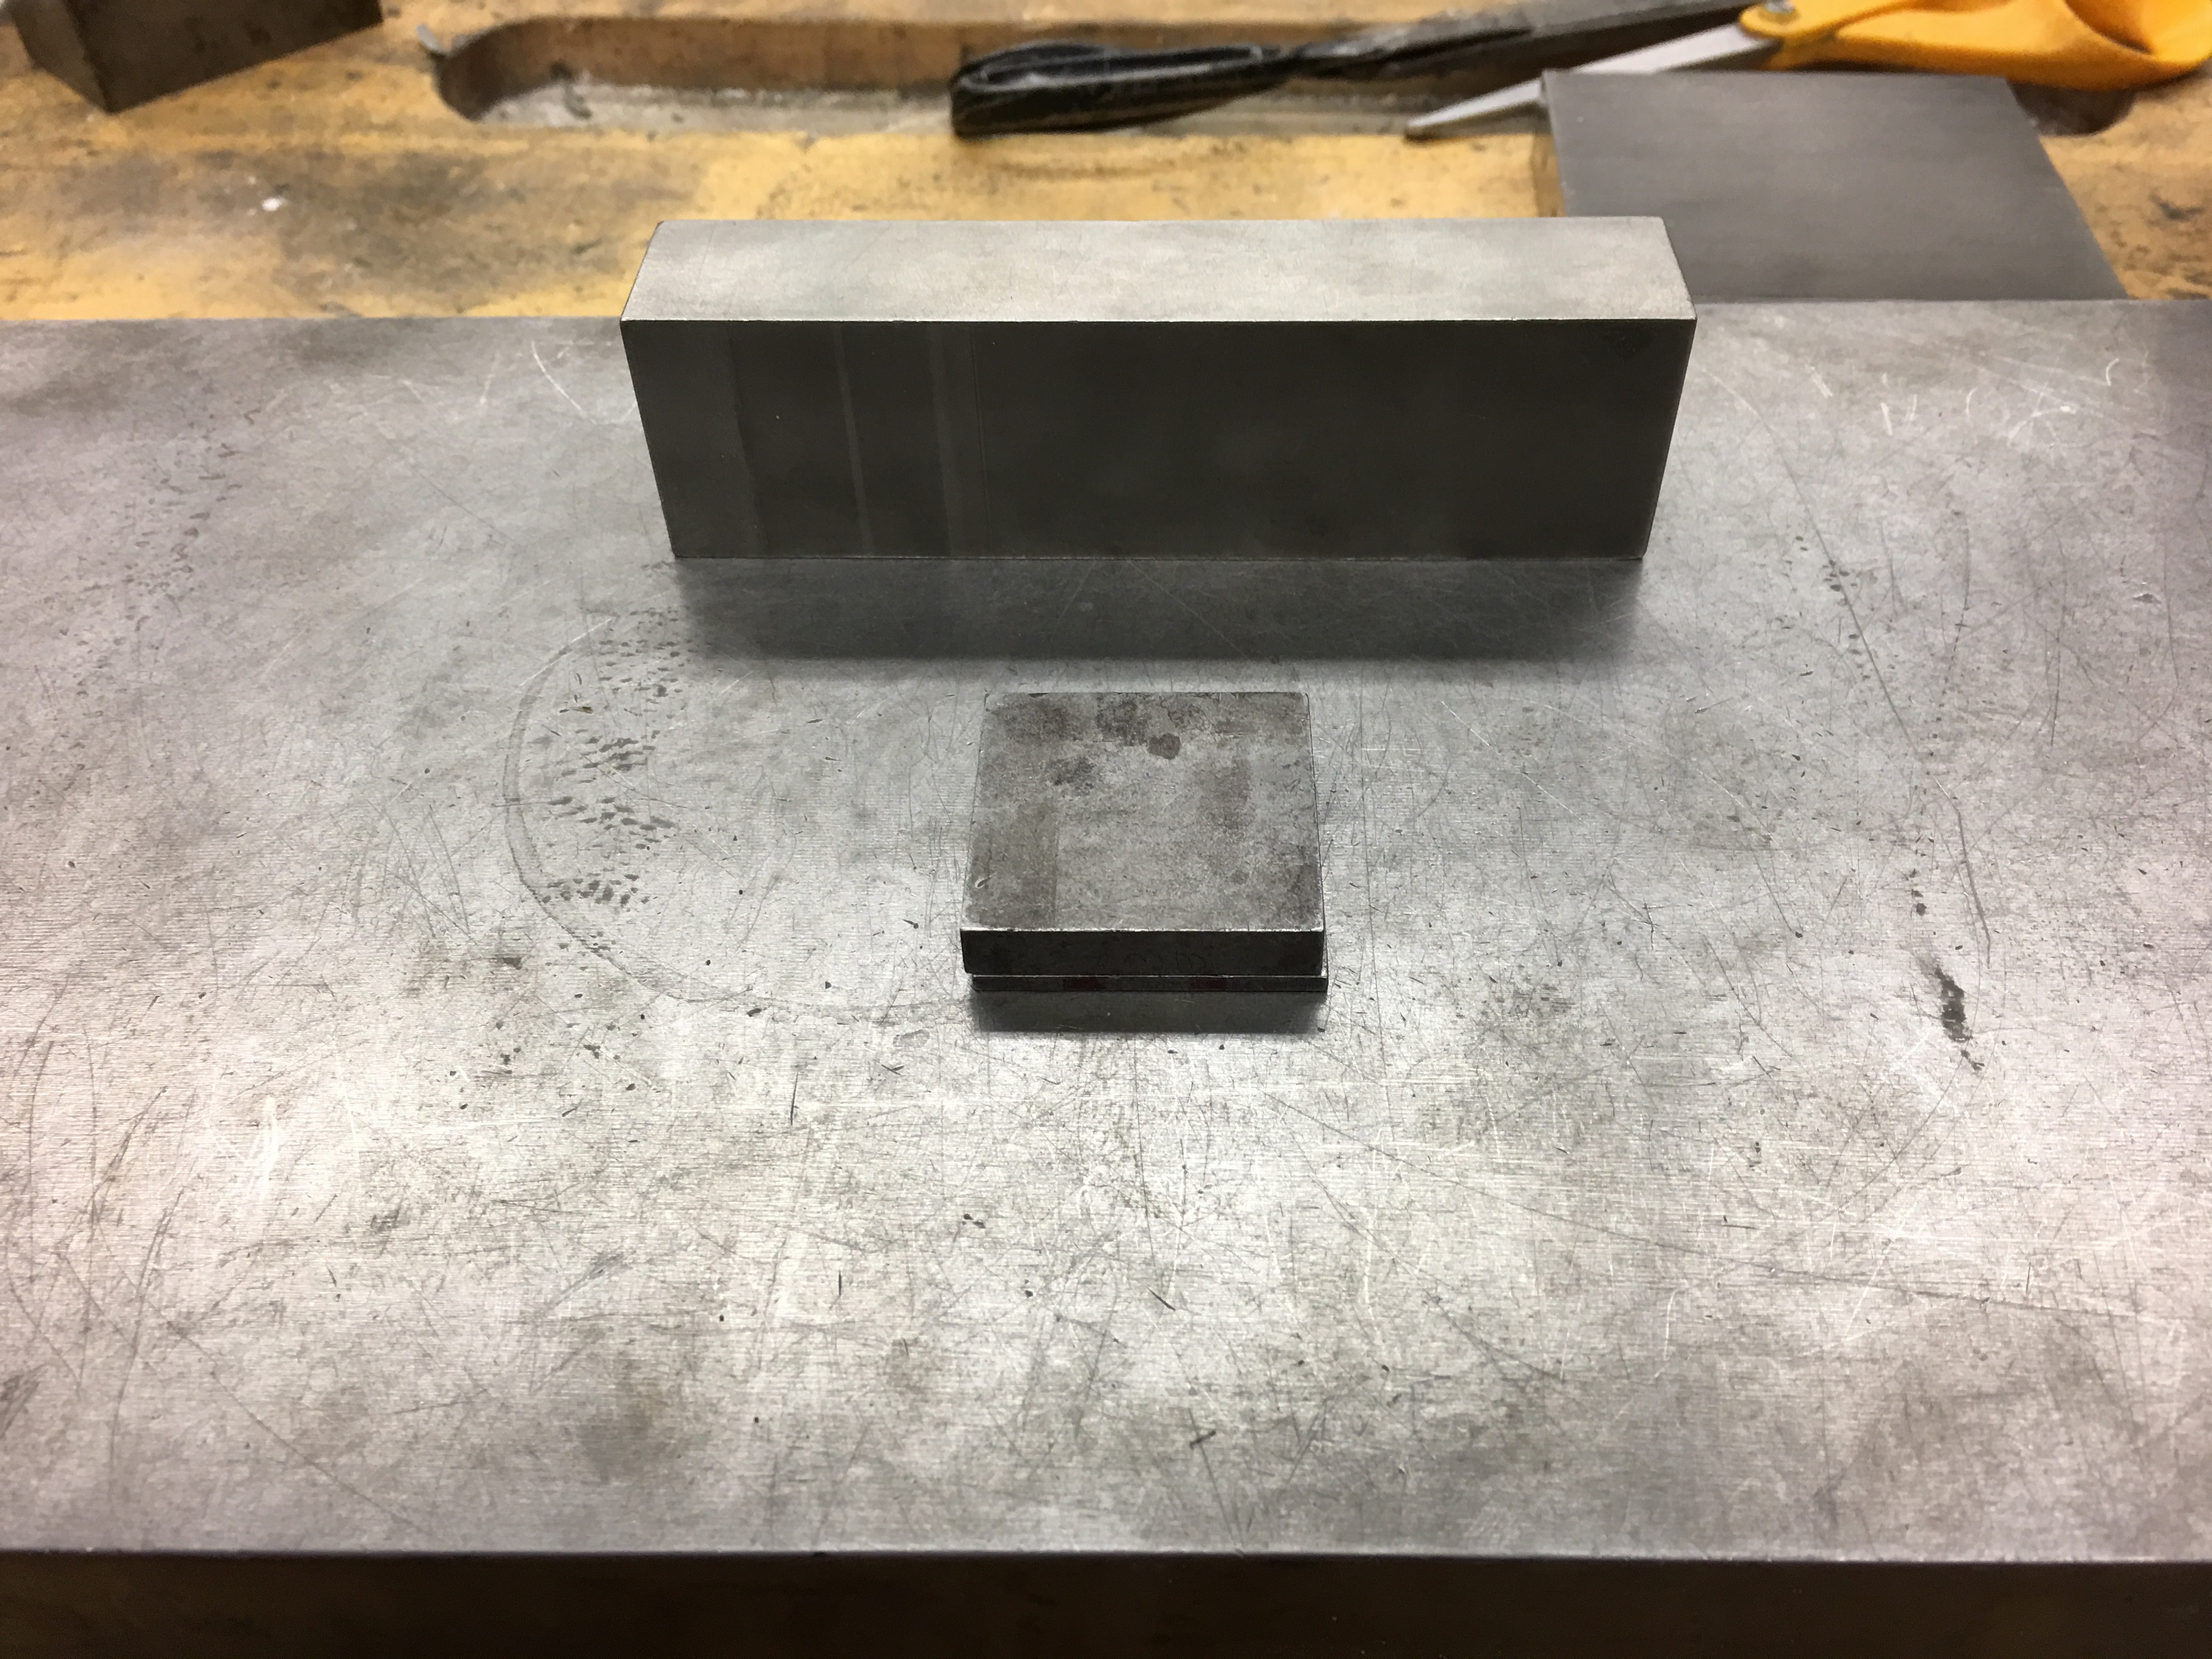
\includegraphics[width=0.7\textwidth]{appendix_sample_prep/dds_thickness_blocks.jpg}
   	\caption{Stack shims to adjust the sample thickness. Note which shims are used.}
  	\label{Fig:dds_thickness_blocks}
\end{figure}
%% End Figure %%

%% Figure %%
\begin{figure}
	\centering
        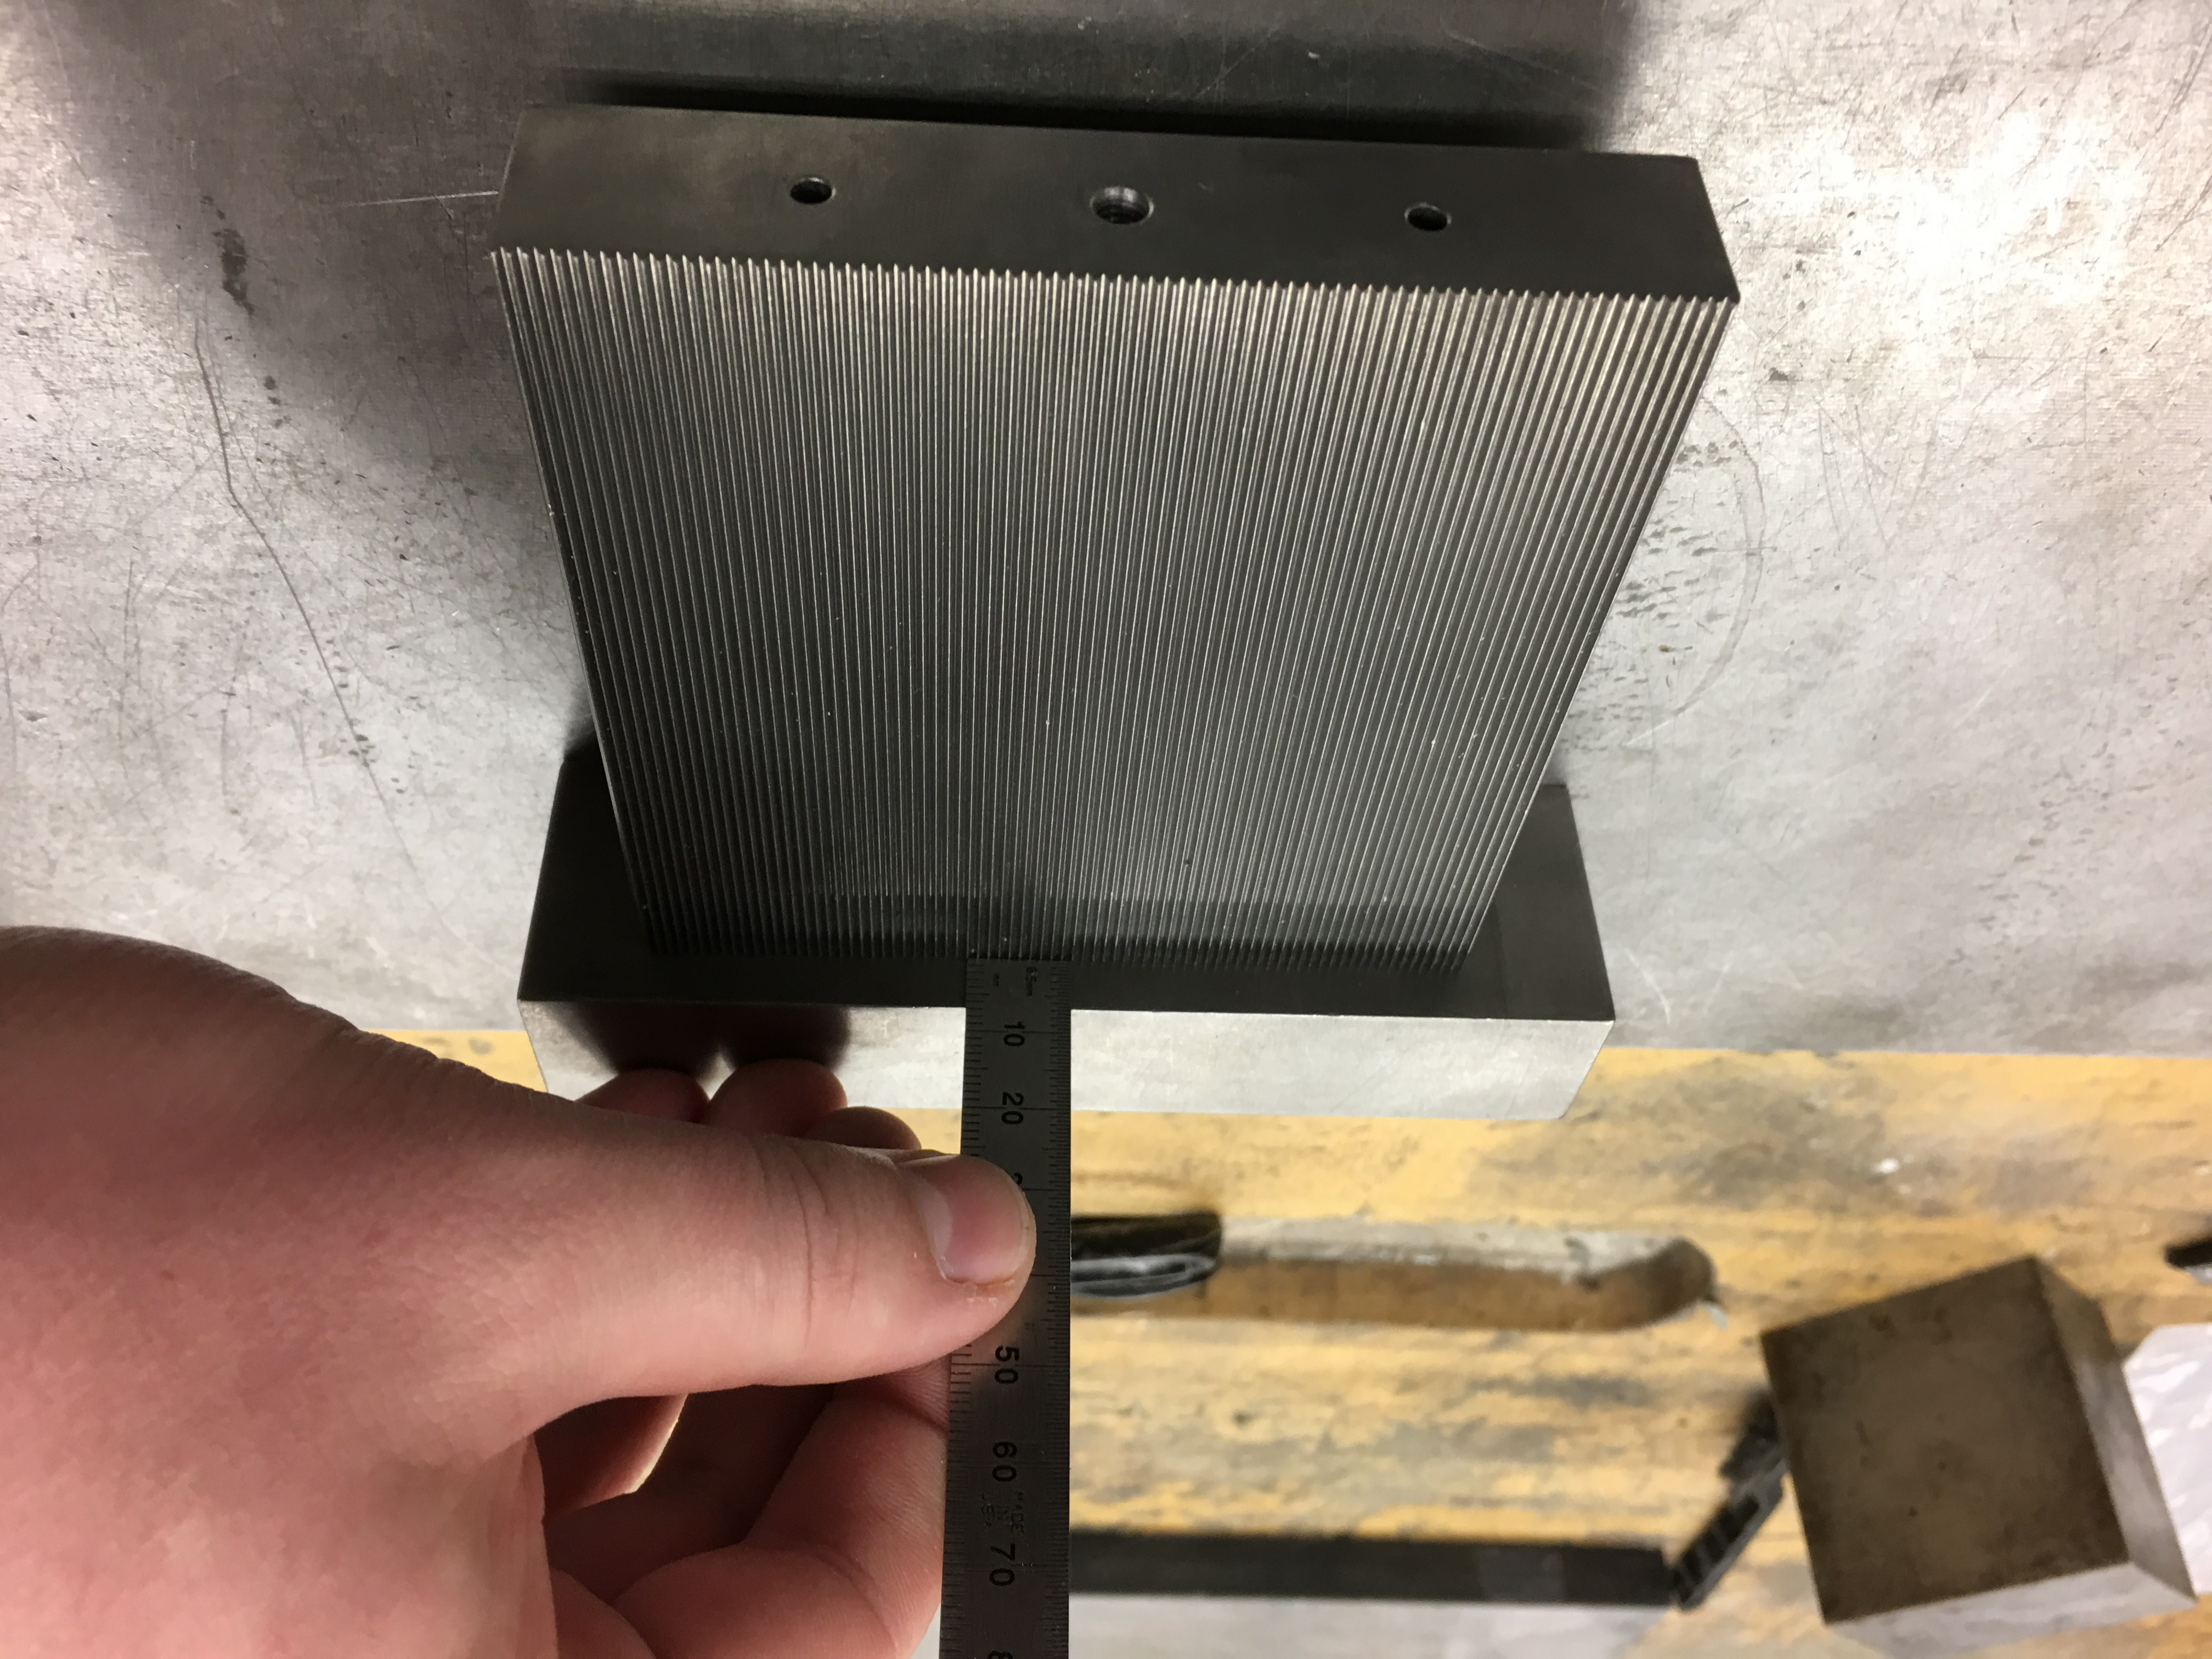
\includegraphics[width=0.7\textwidth]{appendix_sample_prep/dds_thickness_meas.jpg}
   	\caption{Measuring the sample thickness with a steel rule.}
  	\label{Fig:dds_thickness_meas}
\end{figure}
%% End Figure %%

%% Figure %%
\begin{figure}
	\centering
        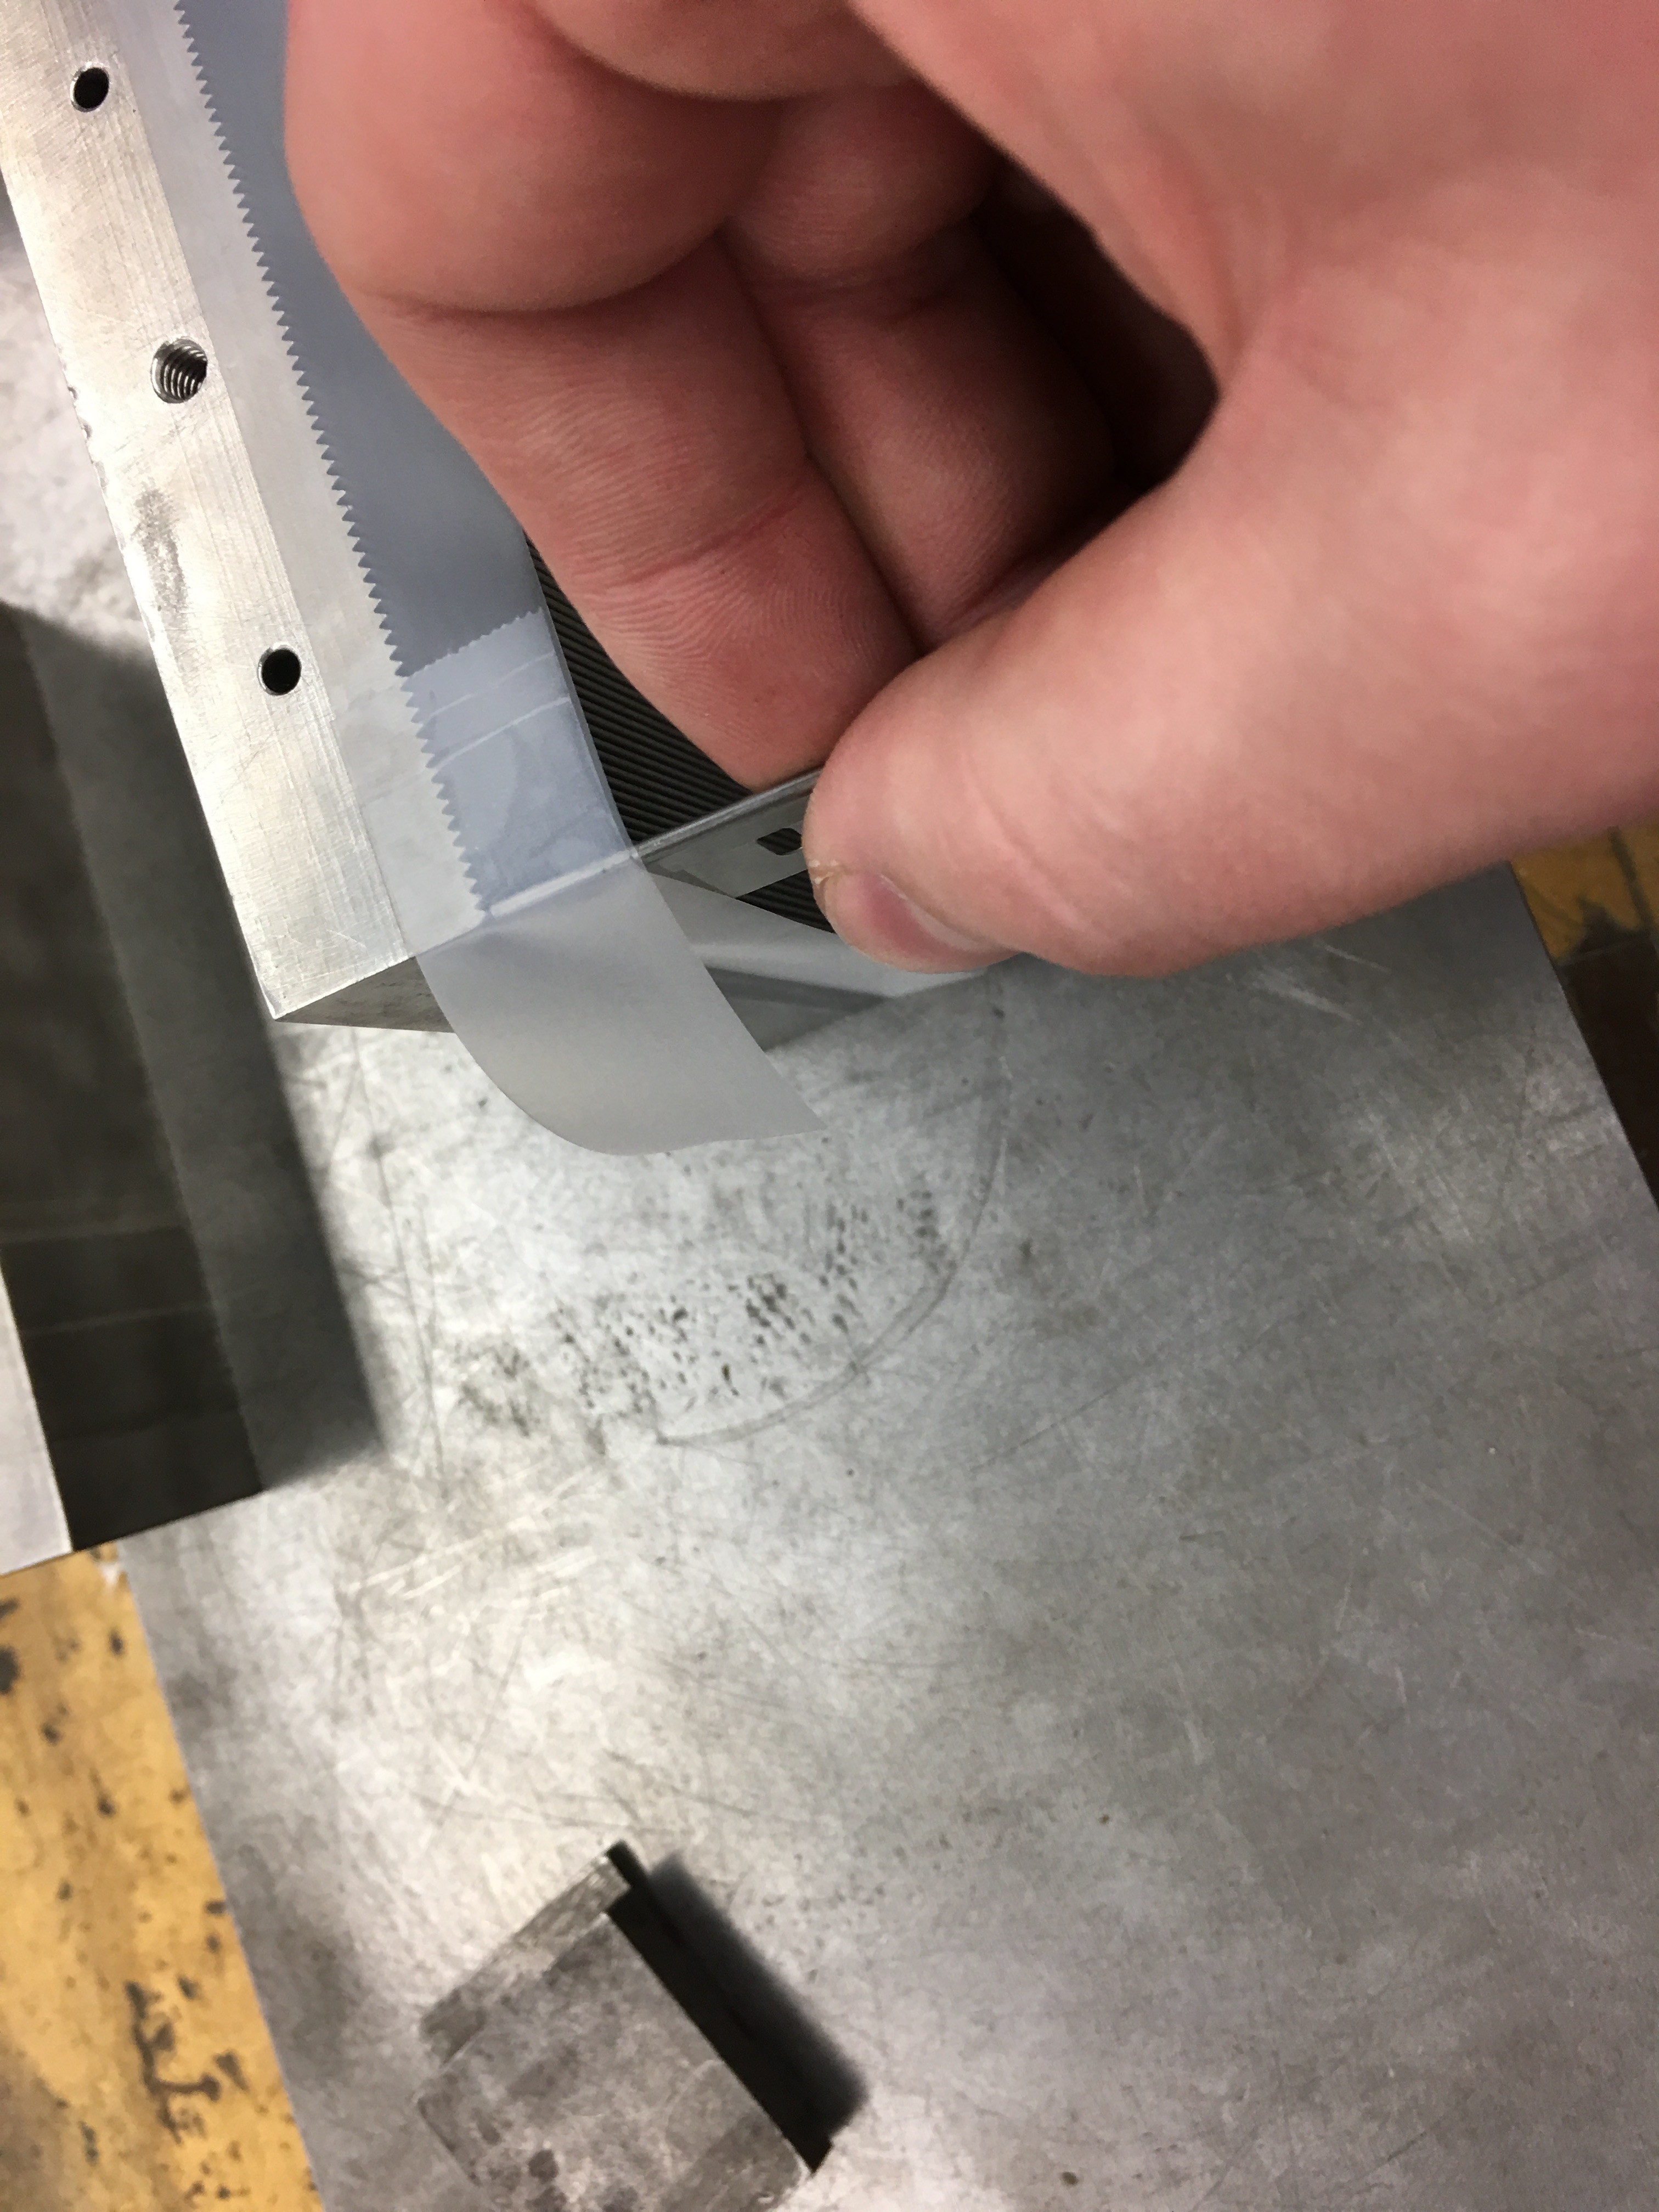
\includegraphics[width=0.7\textwidth]{appendix_sample_prep/dds_wrap_trim.jpg}
   	\caption{Carefully fold over the corner of the tape and trim any excess length.}
  	\label{Fig:dds_wrap_trim}
\end{figure}
%% End Figure %%

\clearpage

%% Figure %%
\begin{figure}
	\centering
        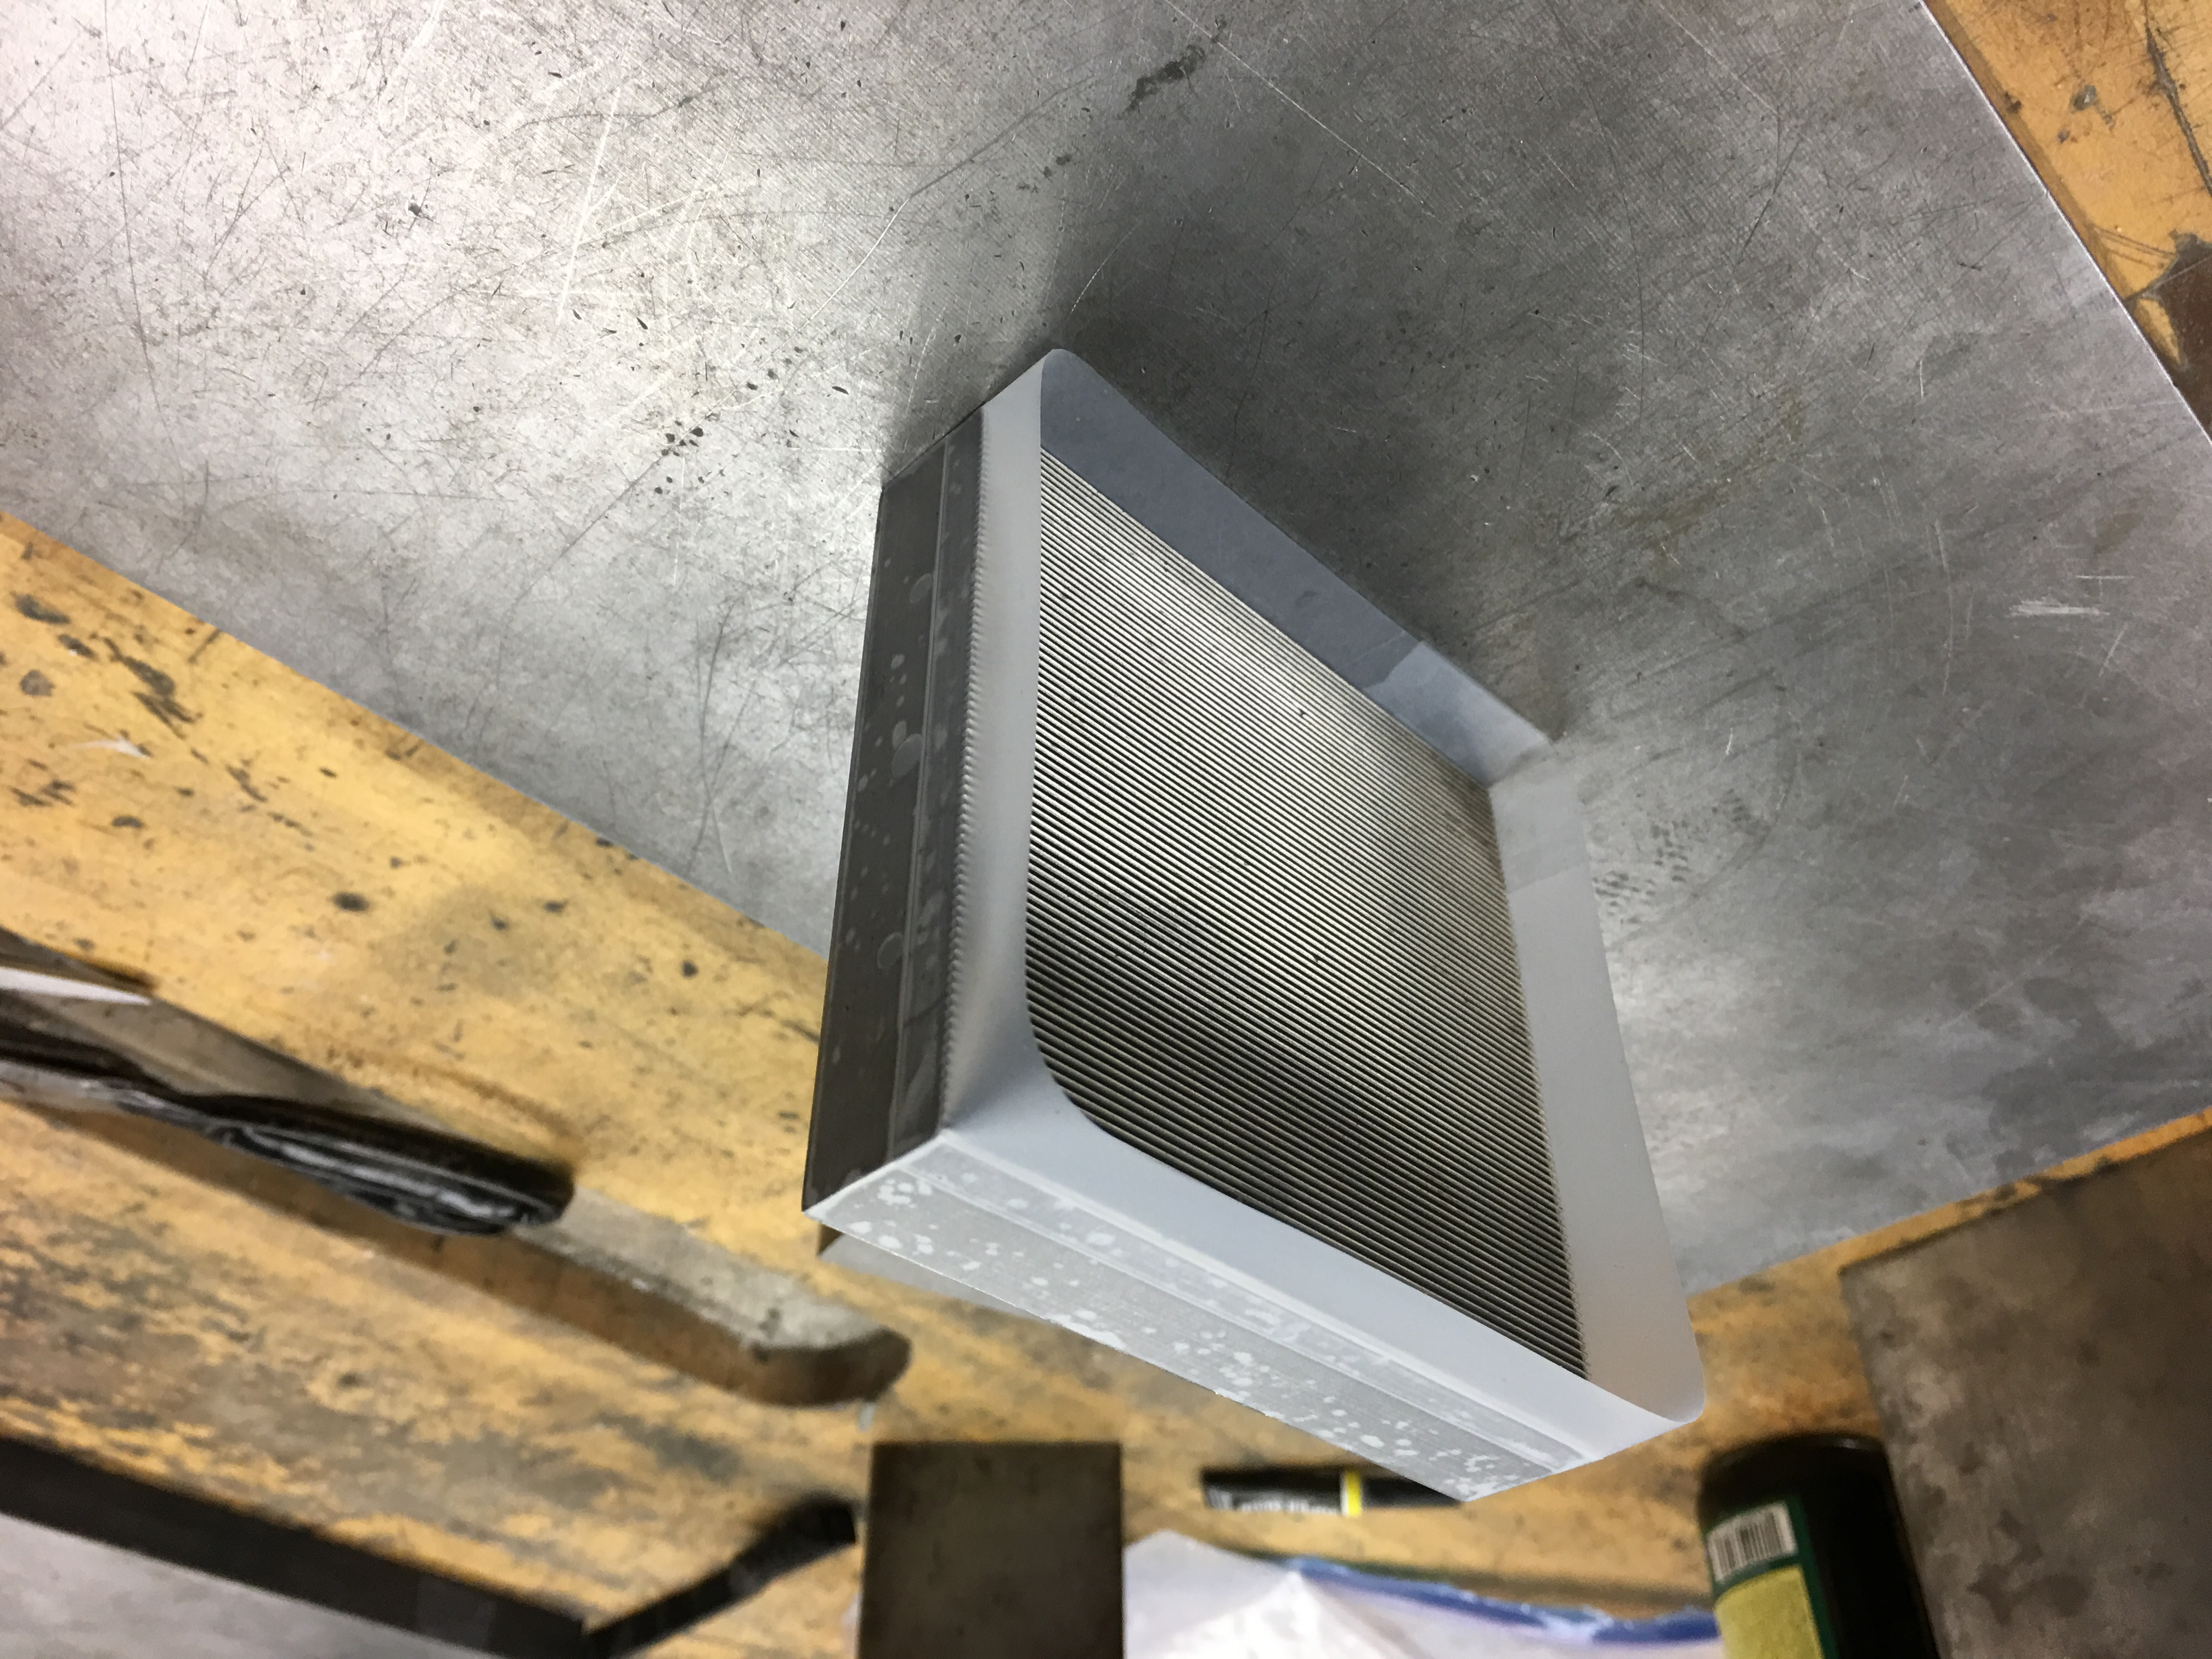
\includegraphics[width=0.7\textwidth]{appendix_sample_prep/dds_two_tape_layers.jpg}
   	\caption{A fully taped side block.}
  	\label{Fig:dds_two_tape_layers}
\end{figure}
%% End Figure %%

%% Figure %%
\begin{figure}
	\centering
        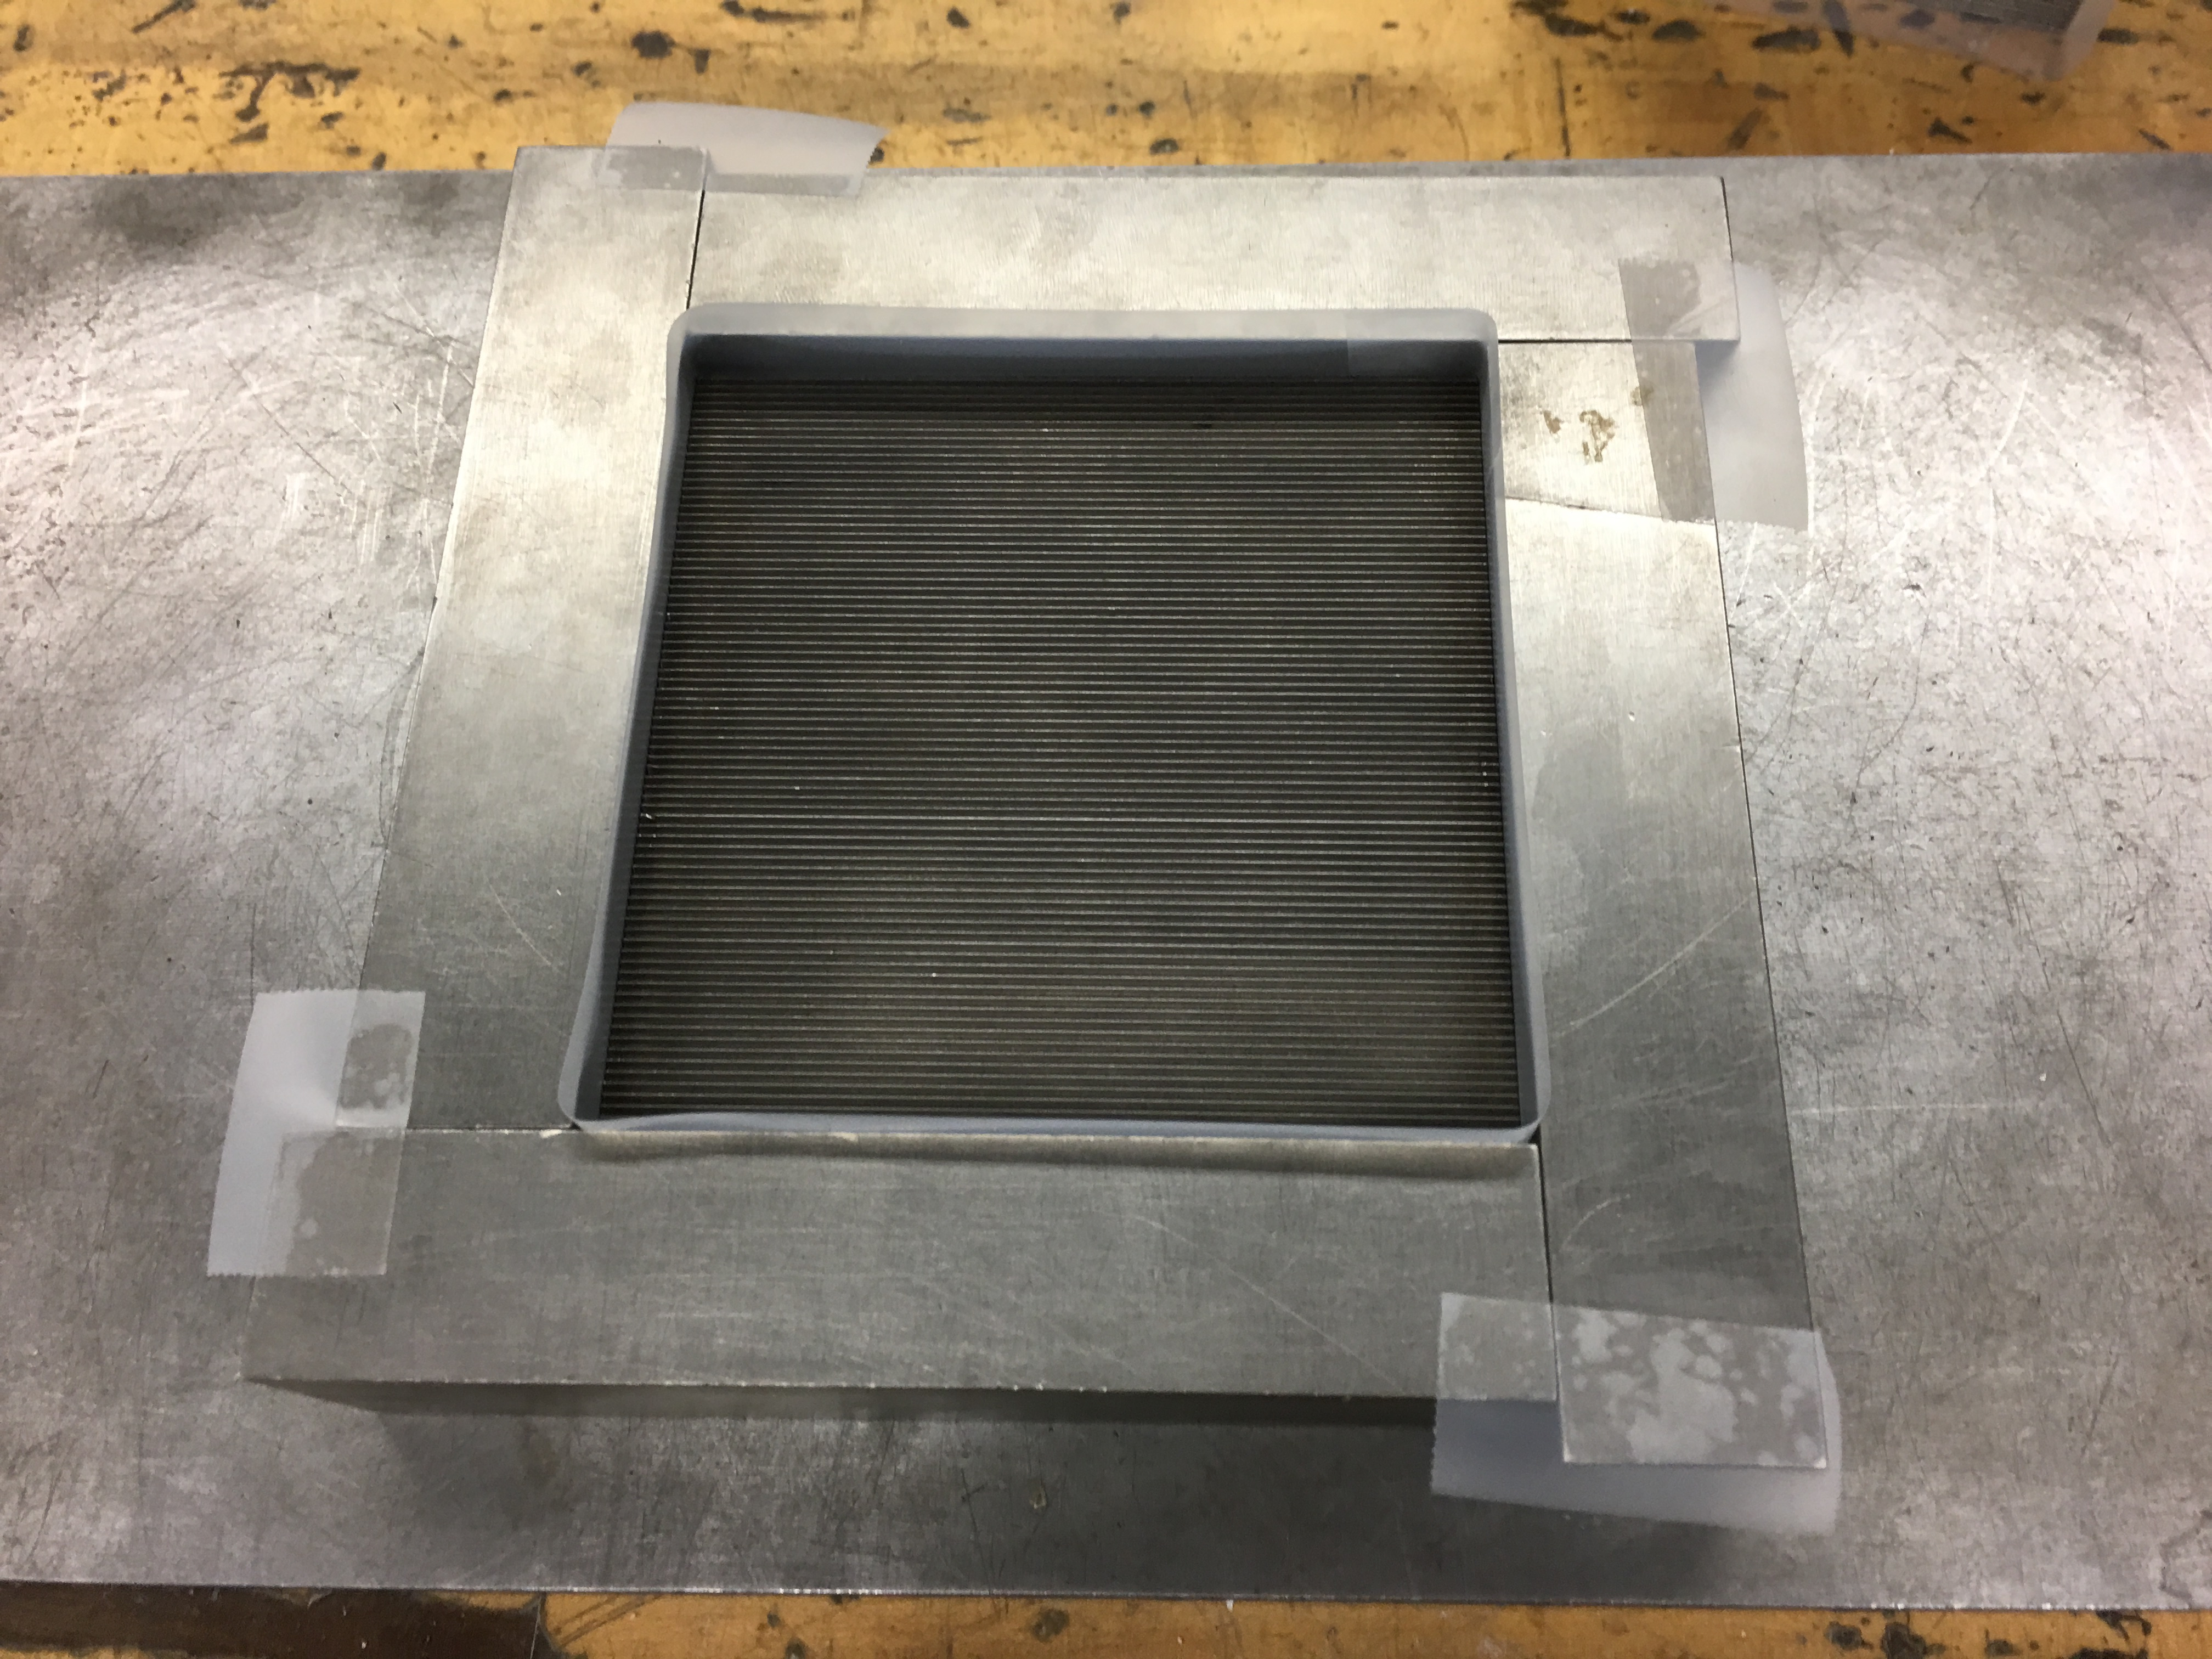
\includegraphics[width=0.7\textwidth]{appendix_sample_prep/dds_trim_setup.jpg}
   	\caption{Setup a jig to trim the excess tape height.}
  	\label{Fig:dds_trim_setup}
\end{figure}
%% End Figure %%

%% Figure %%
\begin{figure}
	\centering
        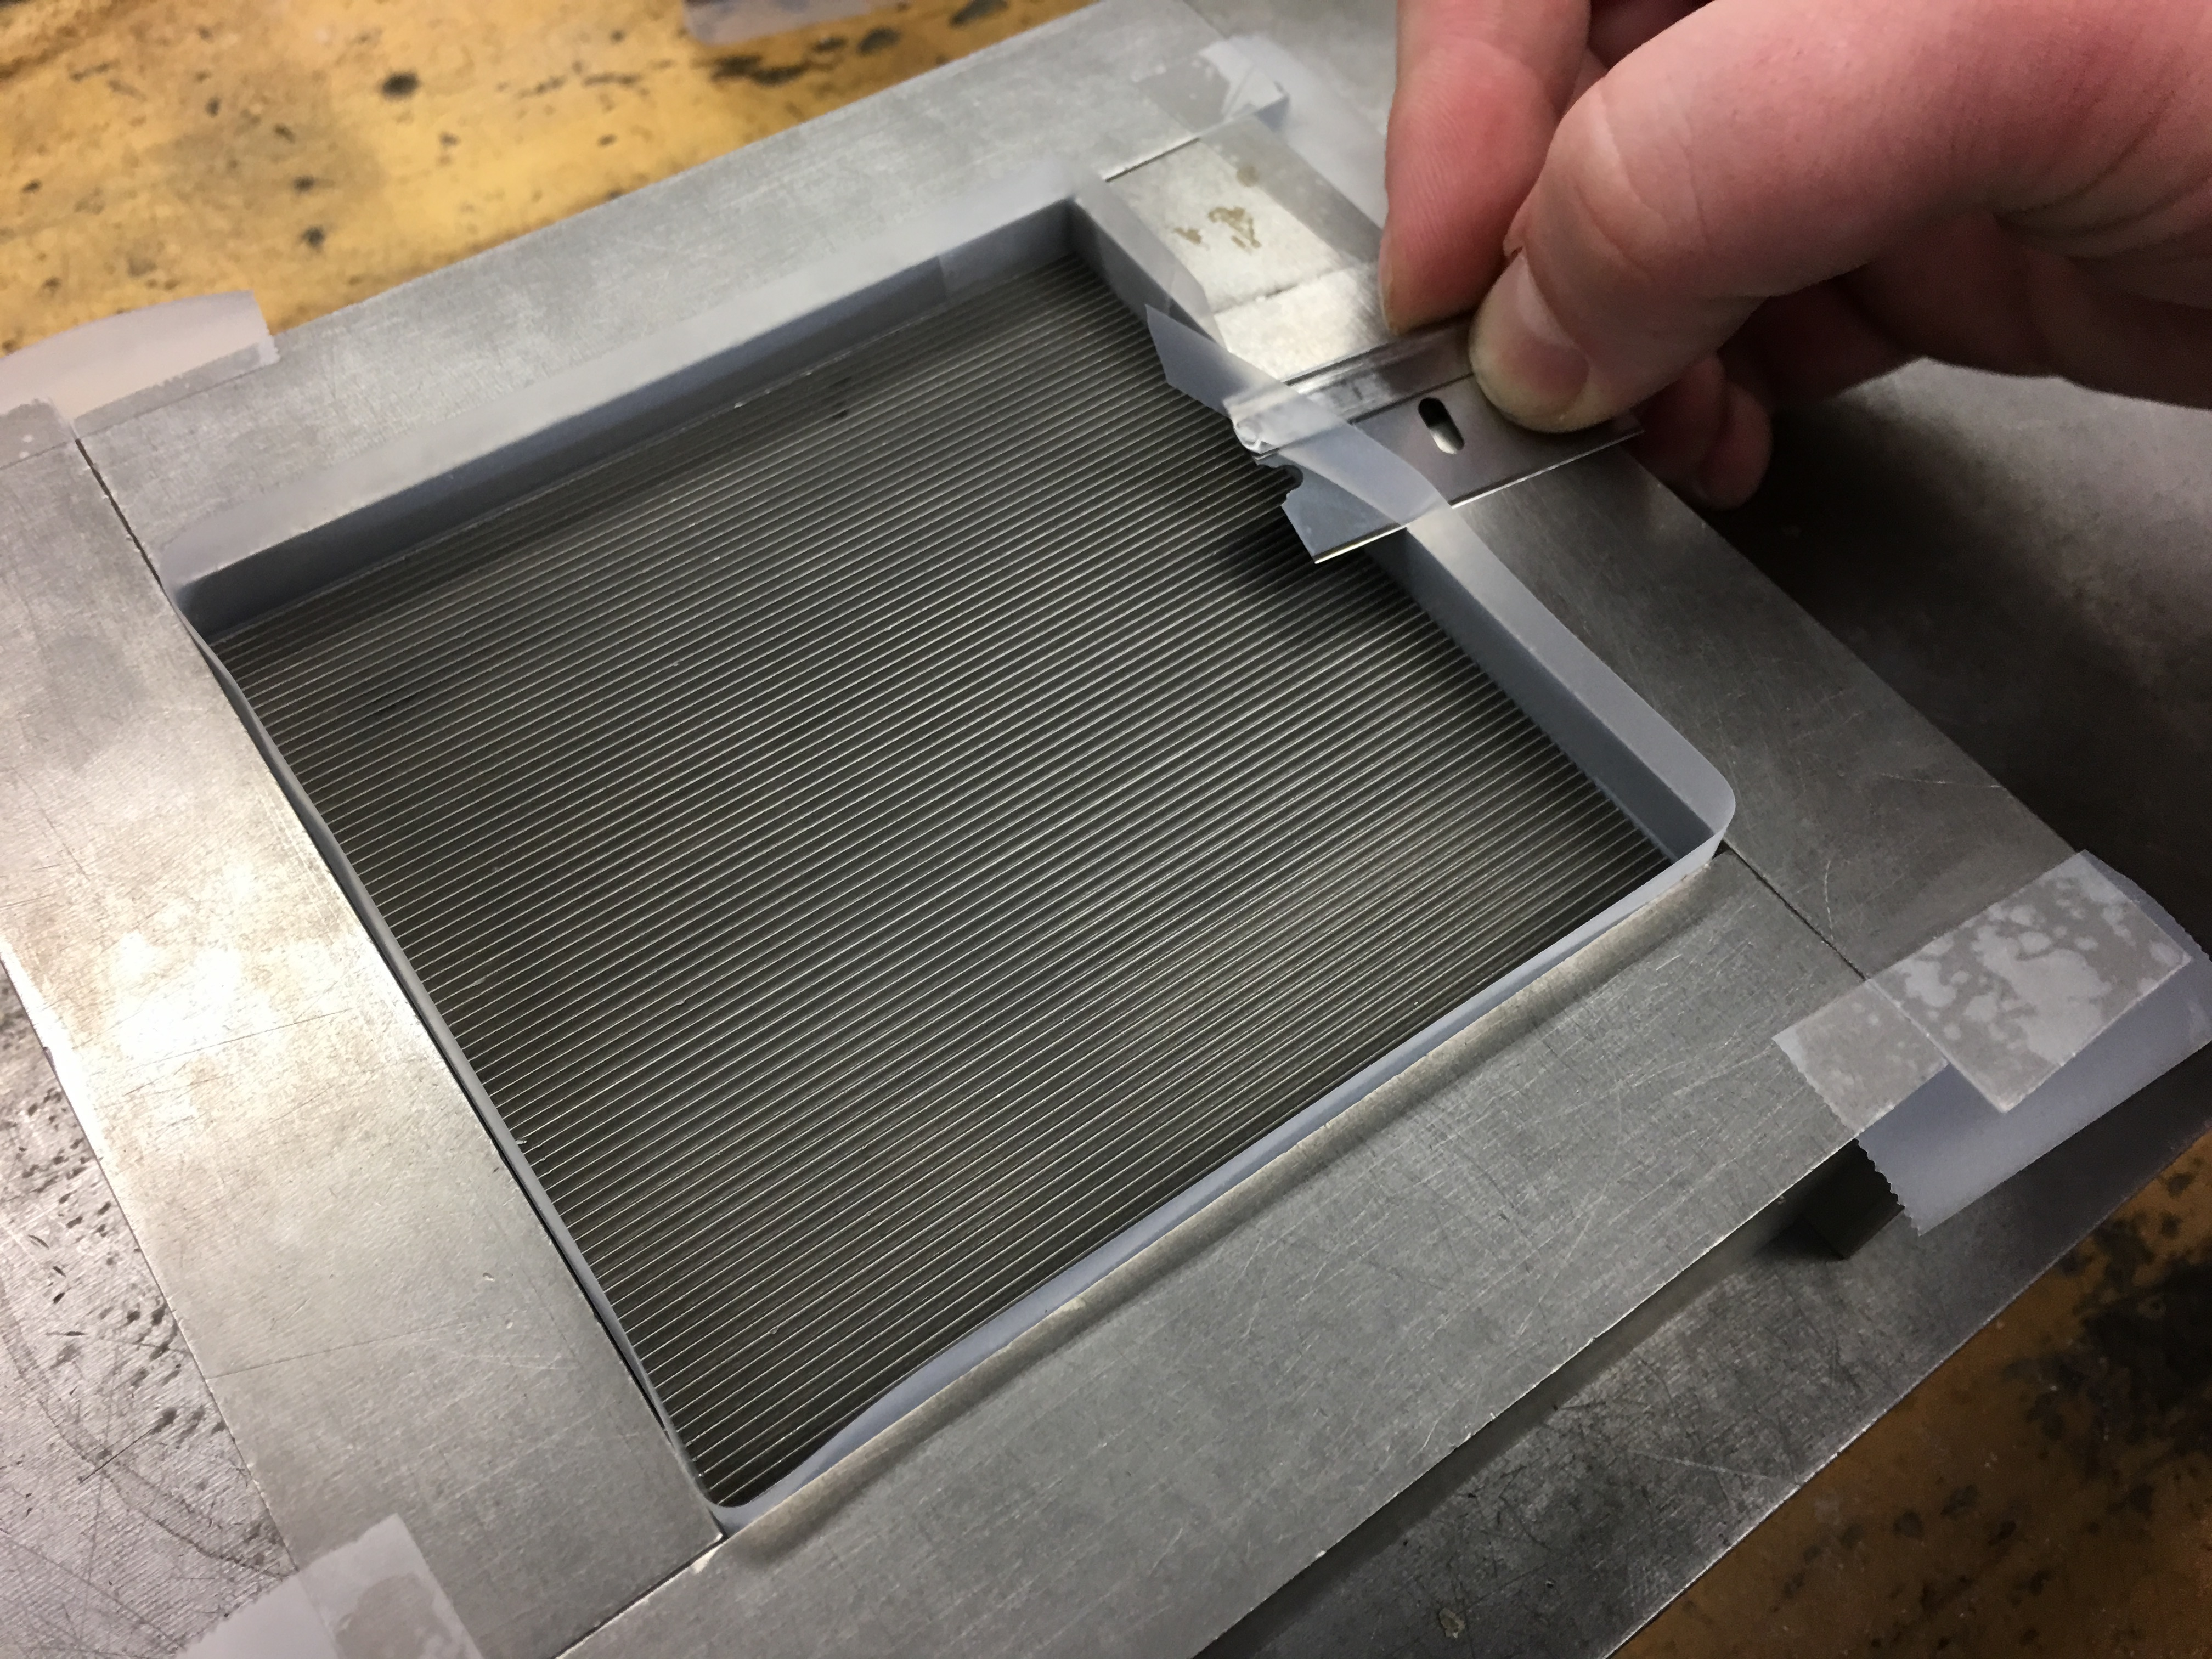
\includegraphics[width=0.7\textwidth]{appendix_sample_prep/dds_tape_trim.jpg}
   	\caption{Carefully trim the tape on all four sides of the block. Note the angle of the razor blade.}
  	\label{Fig:dds_tape_trim}
\end{figure}
%% End Figure %%

%% Figure %%
\begin{figure}
	\centering
        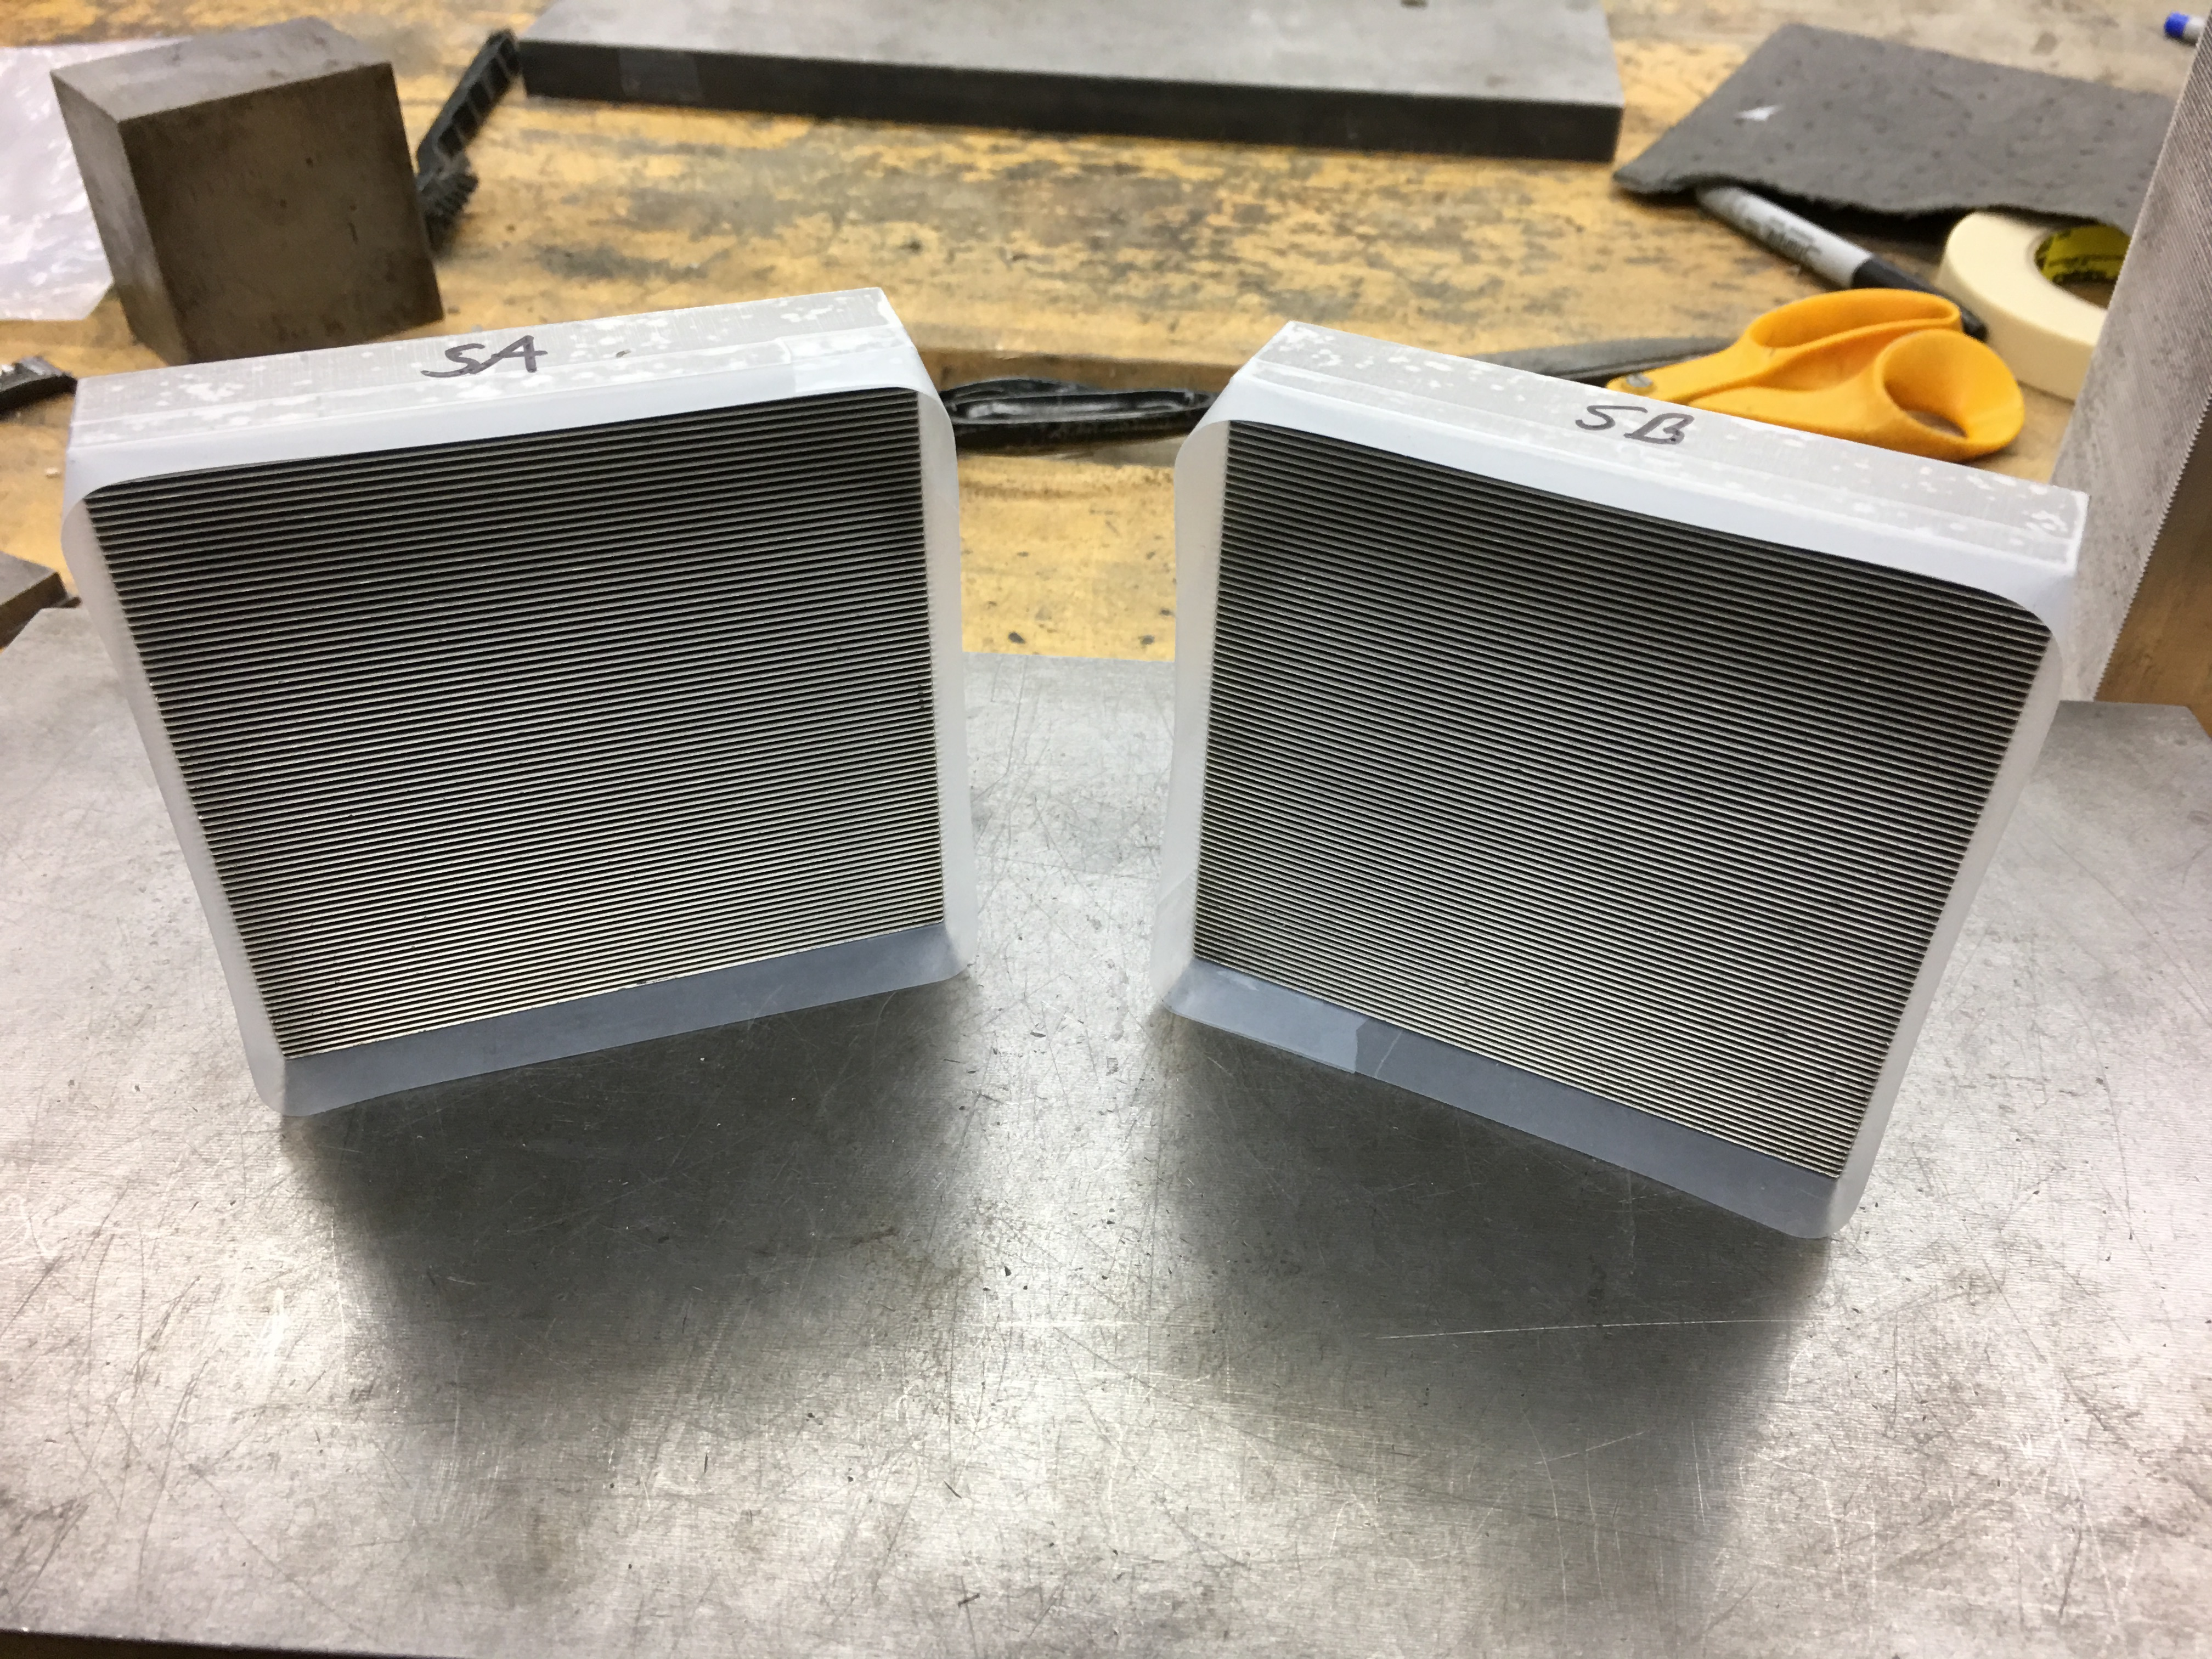
\includegraphics[width=0.7\textwidth]{appendix_sample_prep/dds_blocks_labeled.jpg}
   	\caption{Label the side blocks to help keep track of the mass of material in each layer.}
  	\label{Fig:dds_blocks_labeled}
\end{figure}
%% End Figure %%

\clearpage

%% Figure %%
\begin{figure}
	\centering
        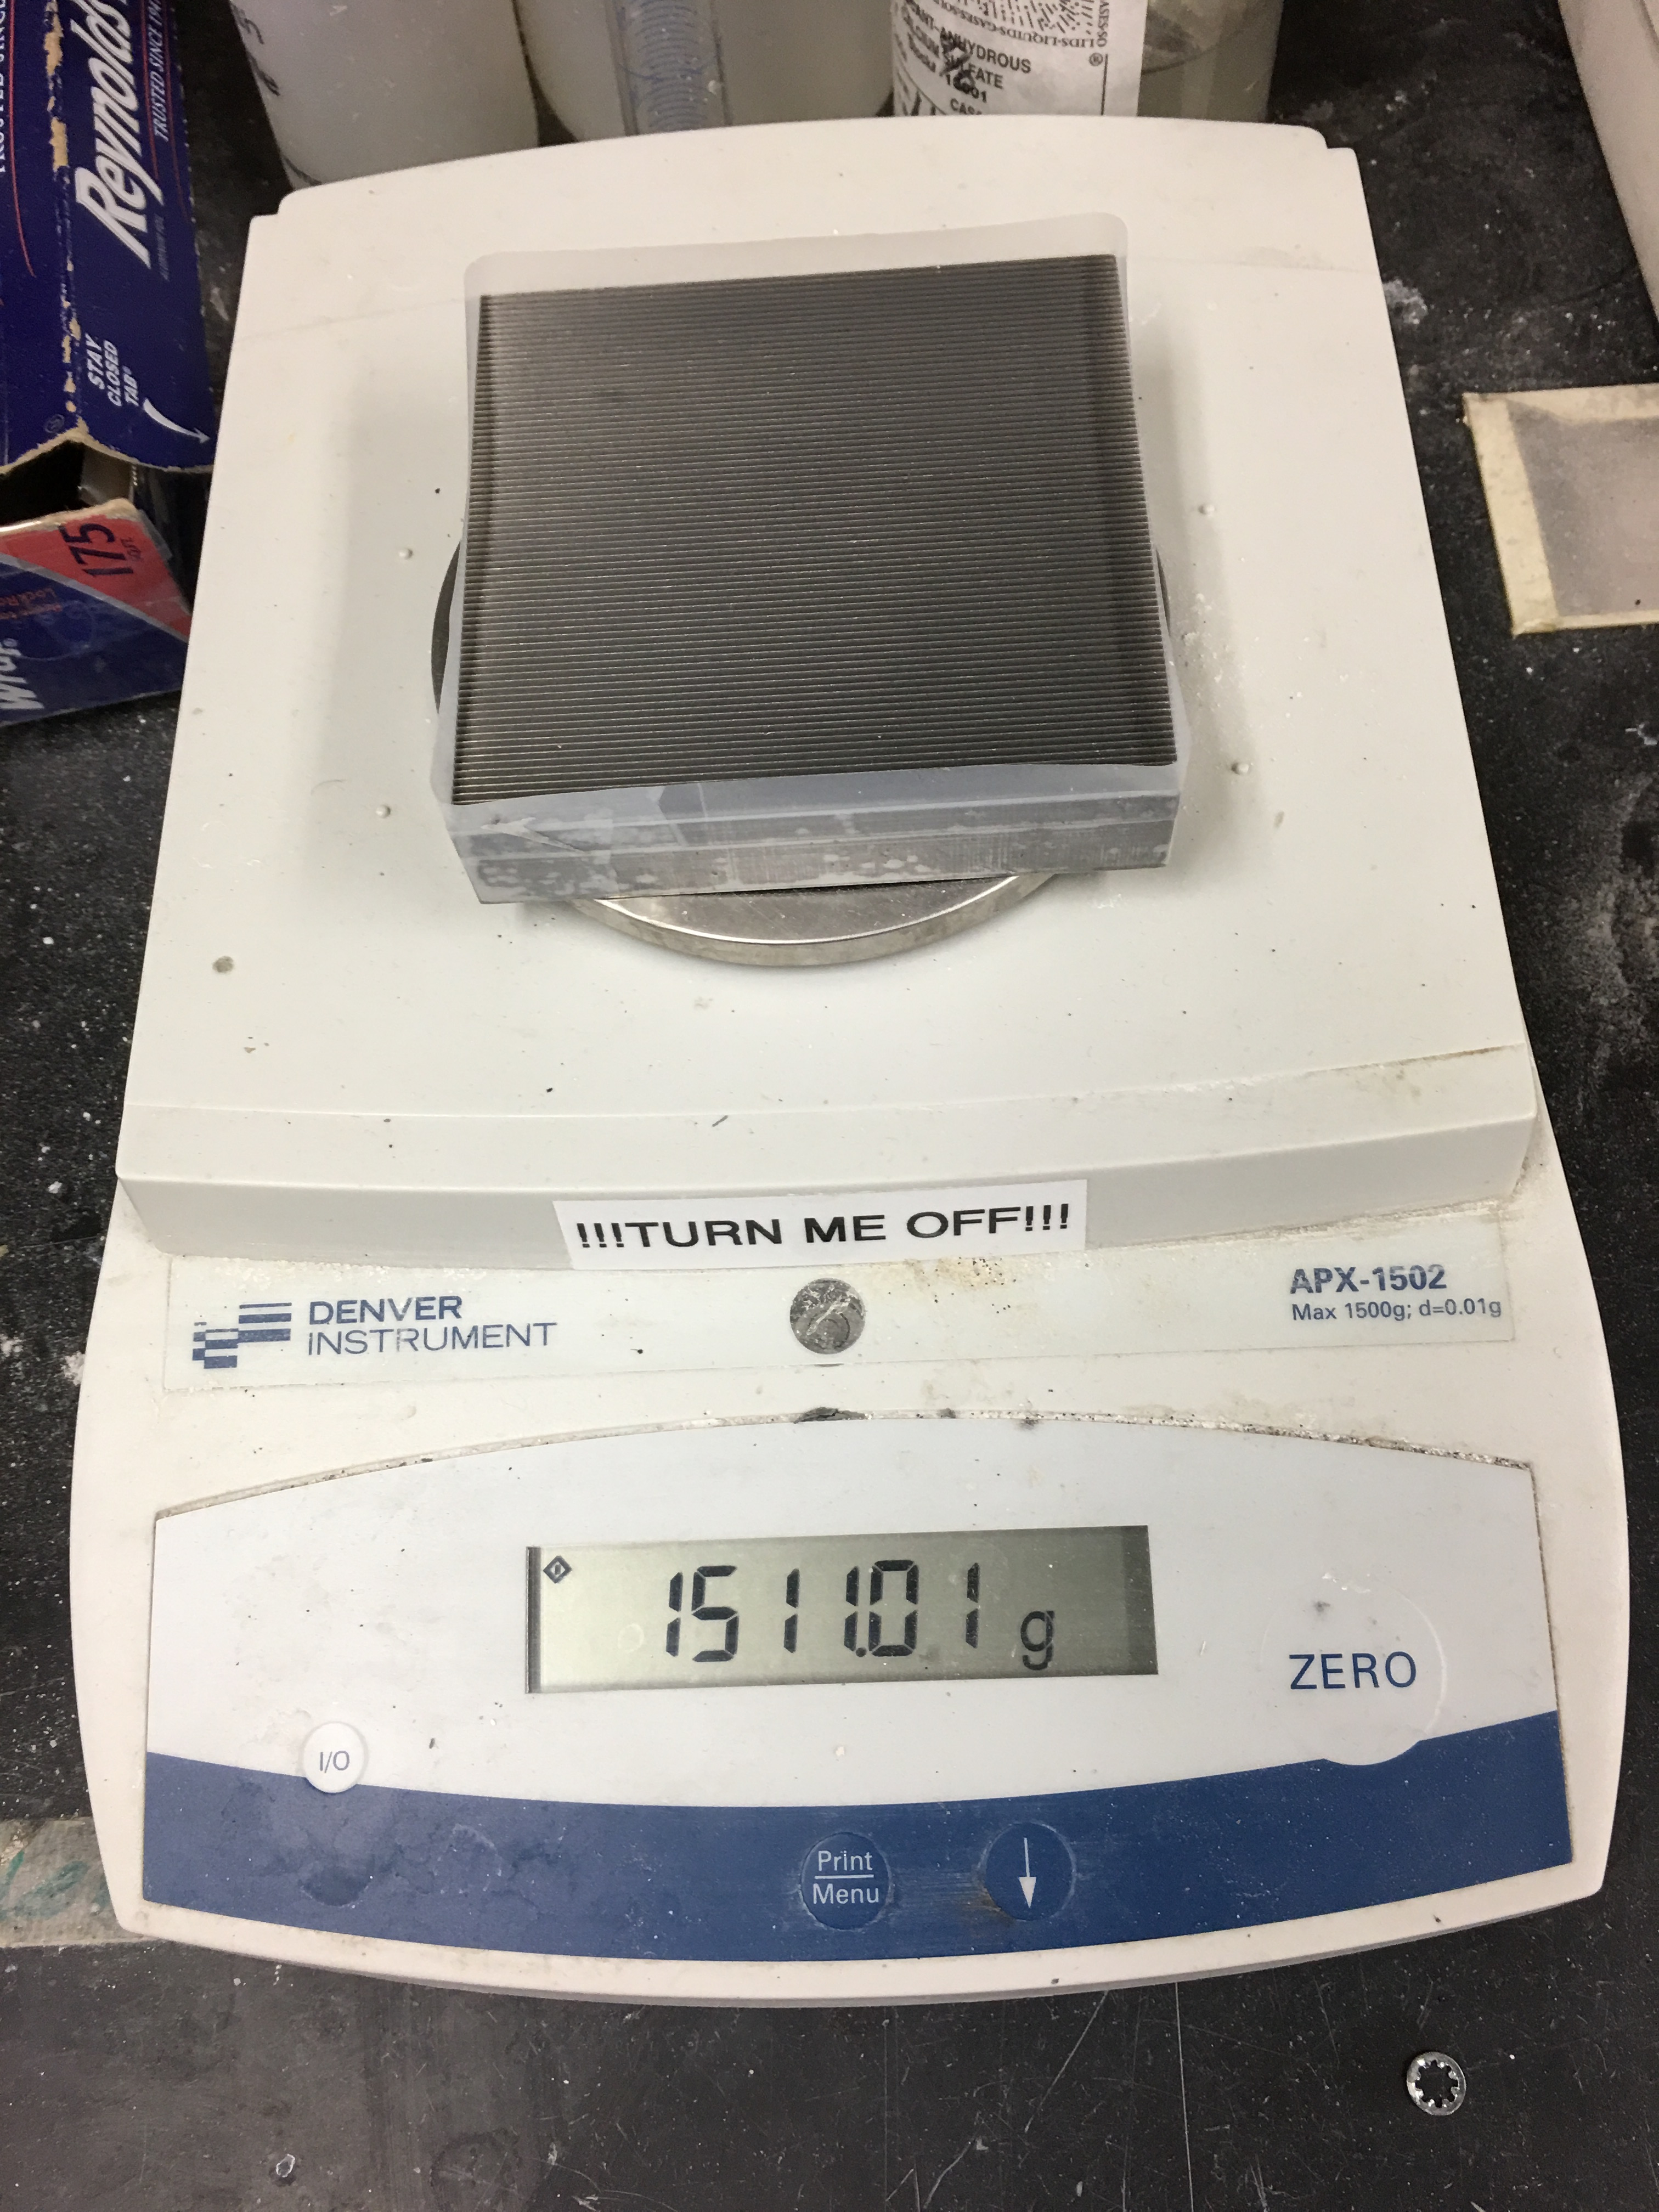
\includegraphics[width=0.7\textwidth]{appendix_sample_prep/dds_block_weight.jpg}
   	\caption{Weigh the blocks after all taping and trimming is completed.}
  	\label{Fig:dds_block_weight}
\end{figure}
%% End Figure %%

%% Figure %%
\begin{figure}
	\centering
        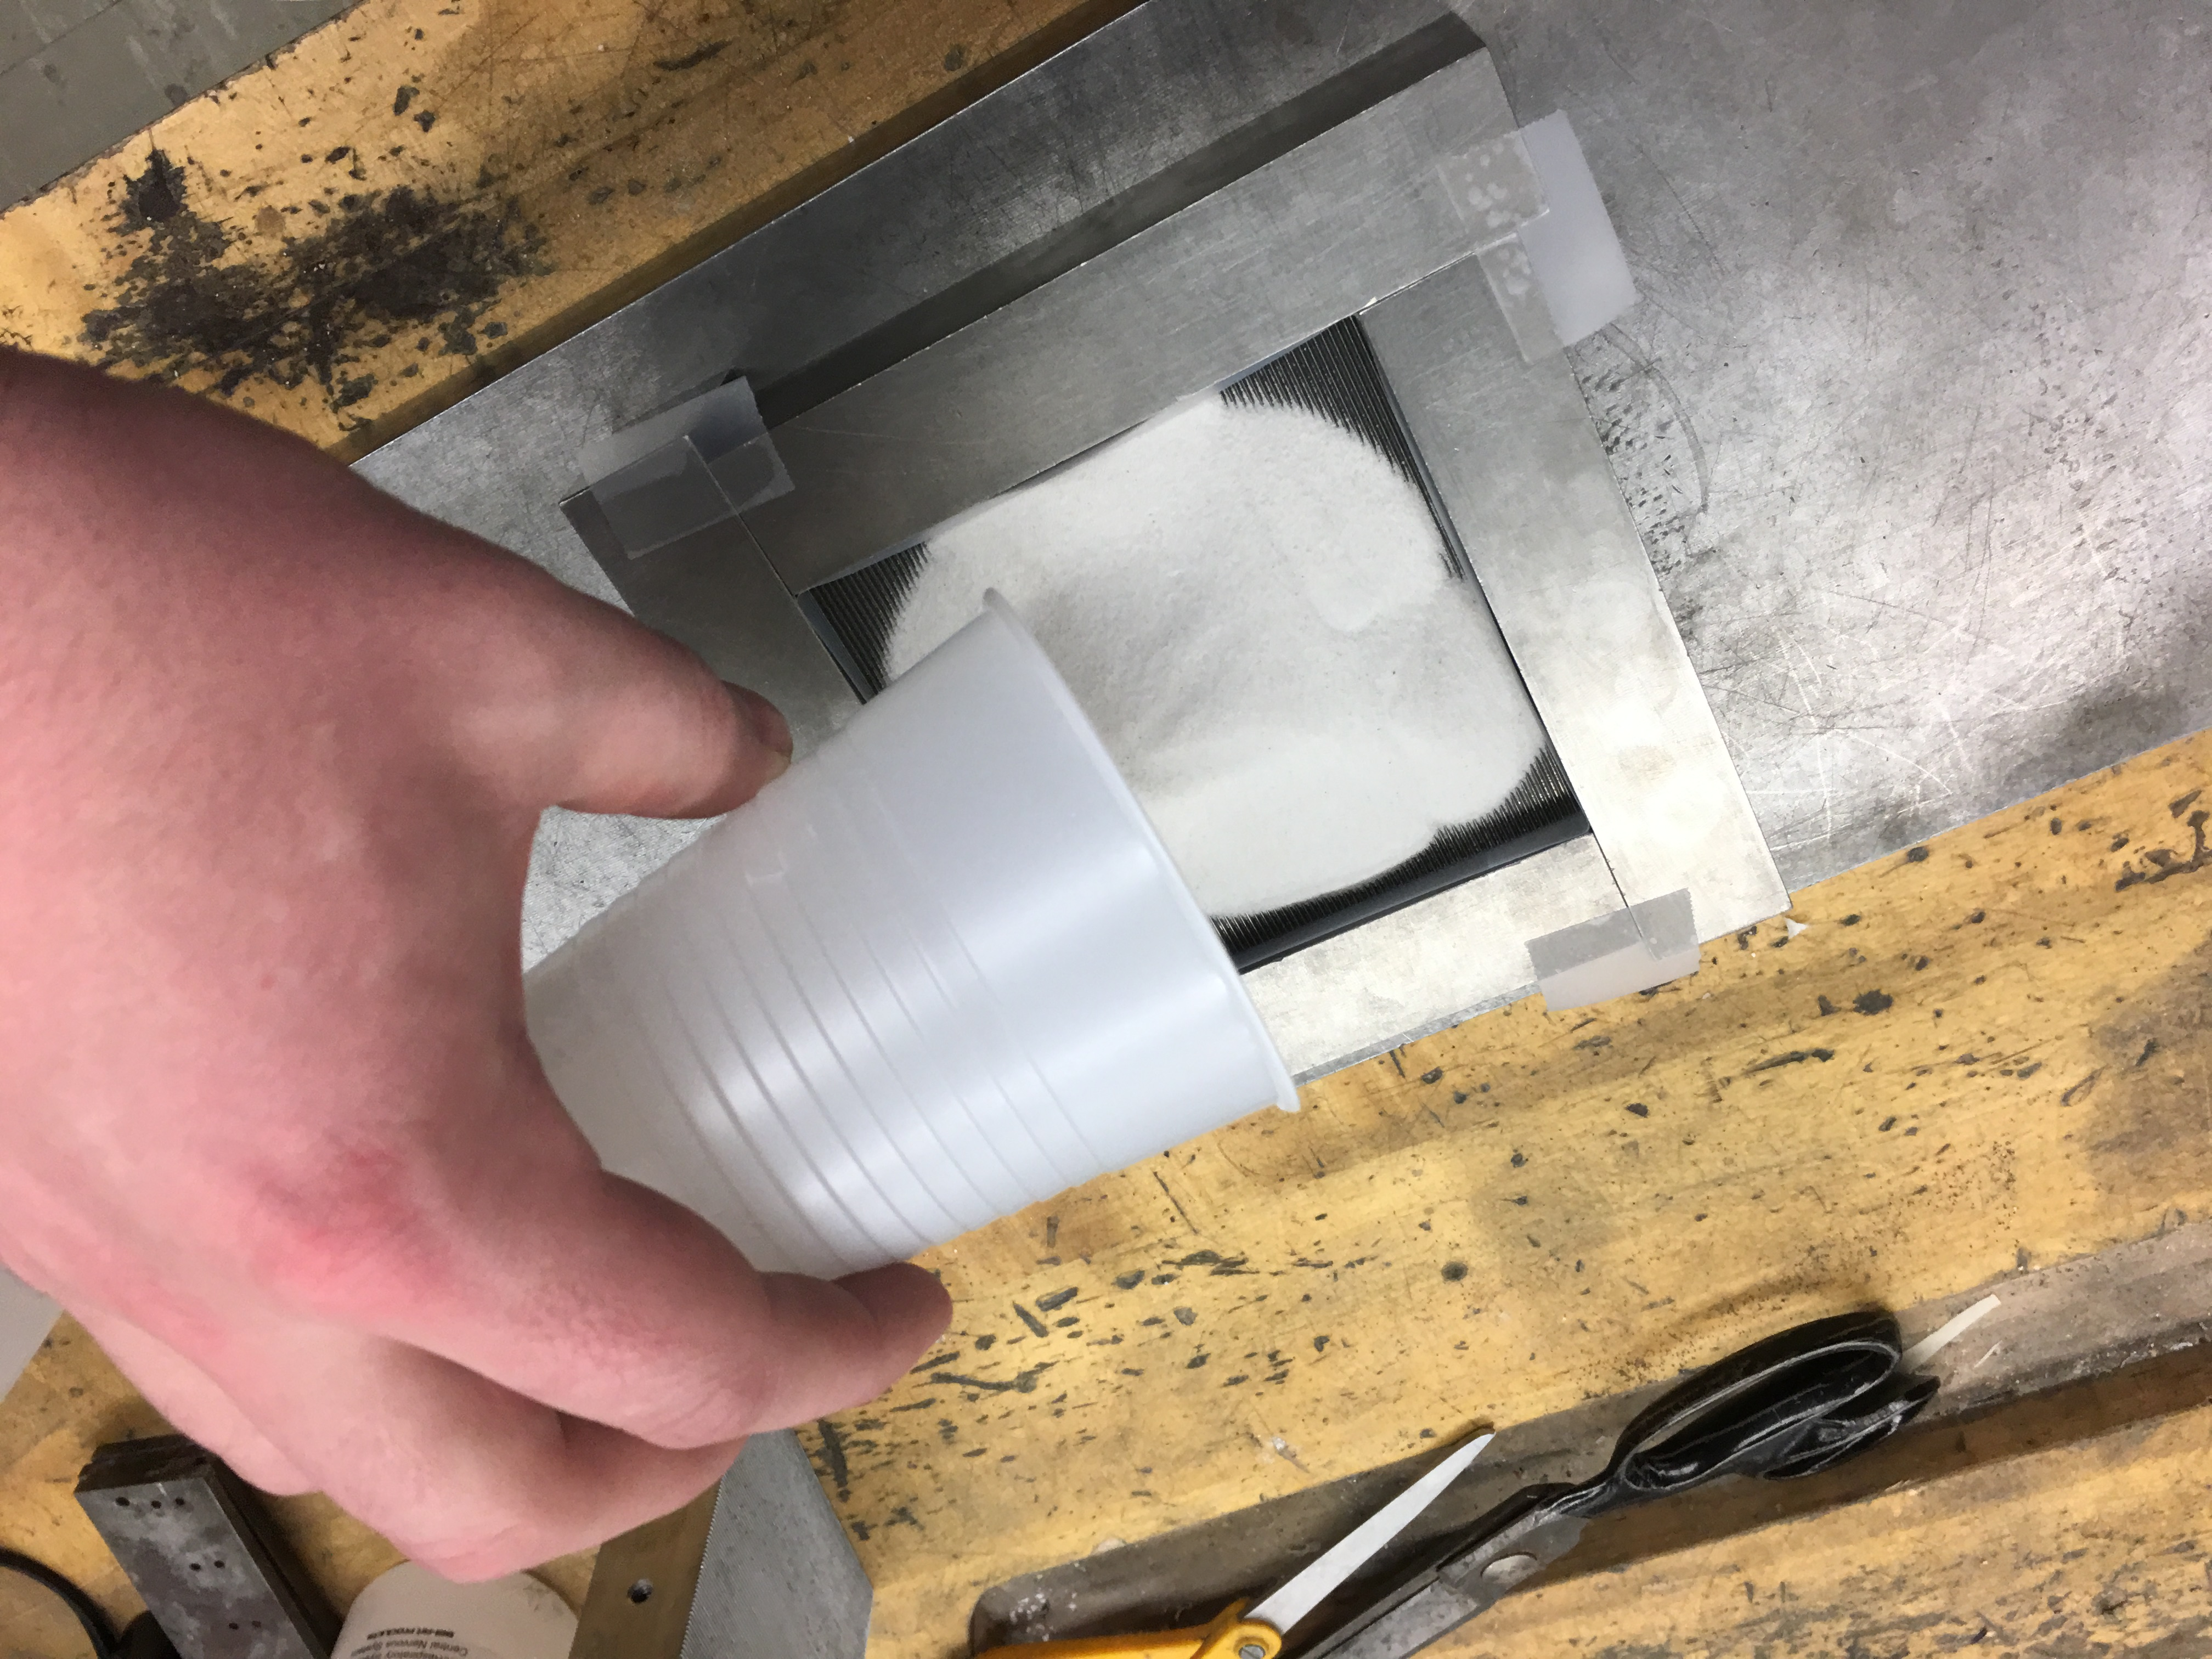
\includegraphics[width=0.7\textwidth]{appendix_sample_prep/dds_pour_material.jpg}
   	\caption{Carefully pour sample material into the taped area of the block.}
  	\label{Fig:dds_pour_material}
\end{figure}
%% End Figure %%

%% Figure %%
\begin{figure}
	\centering
        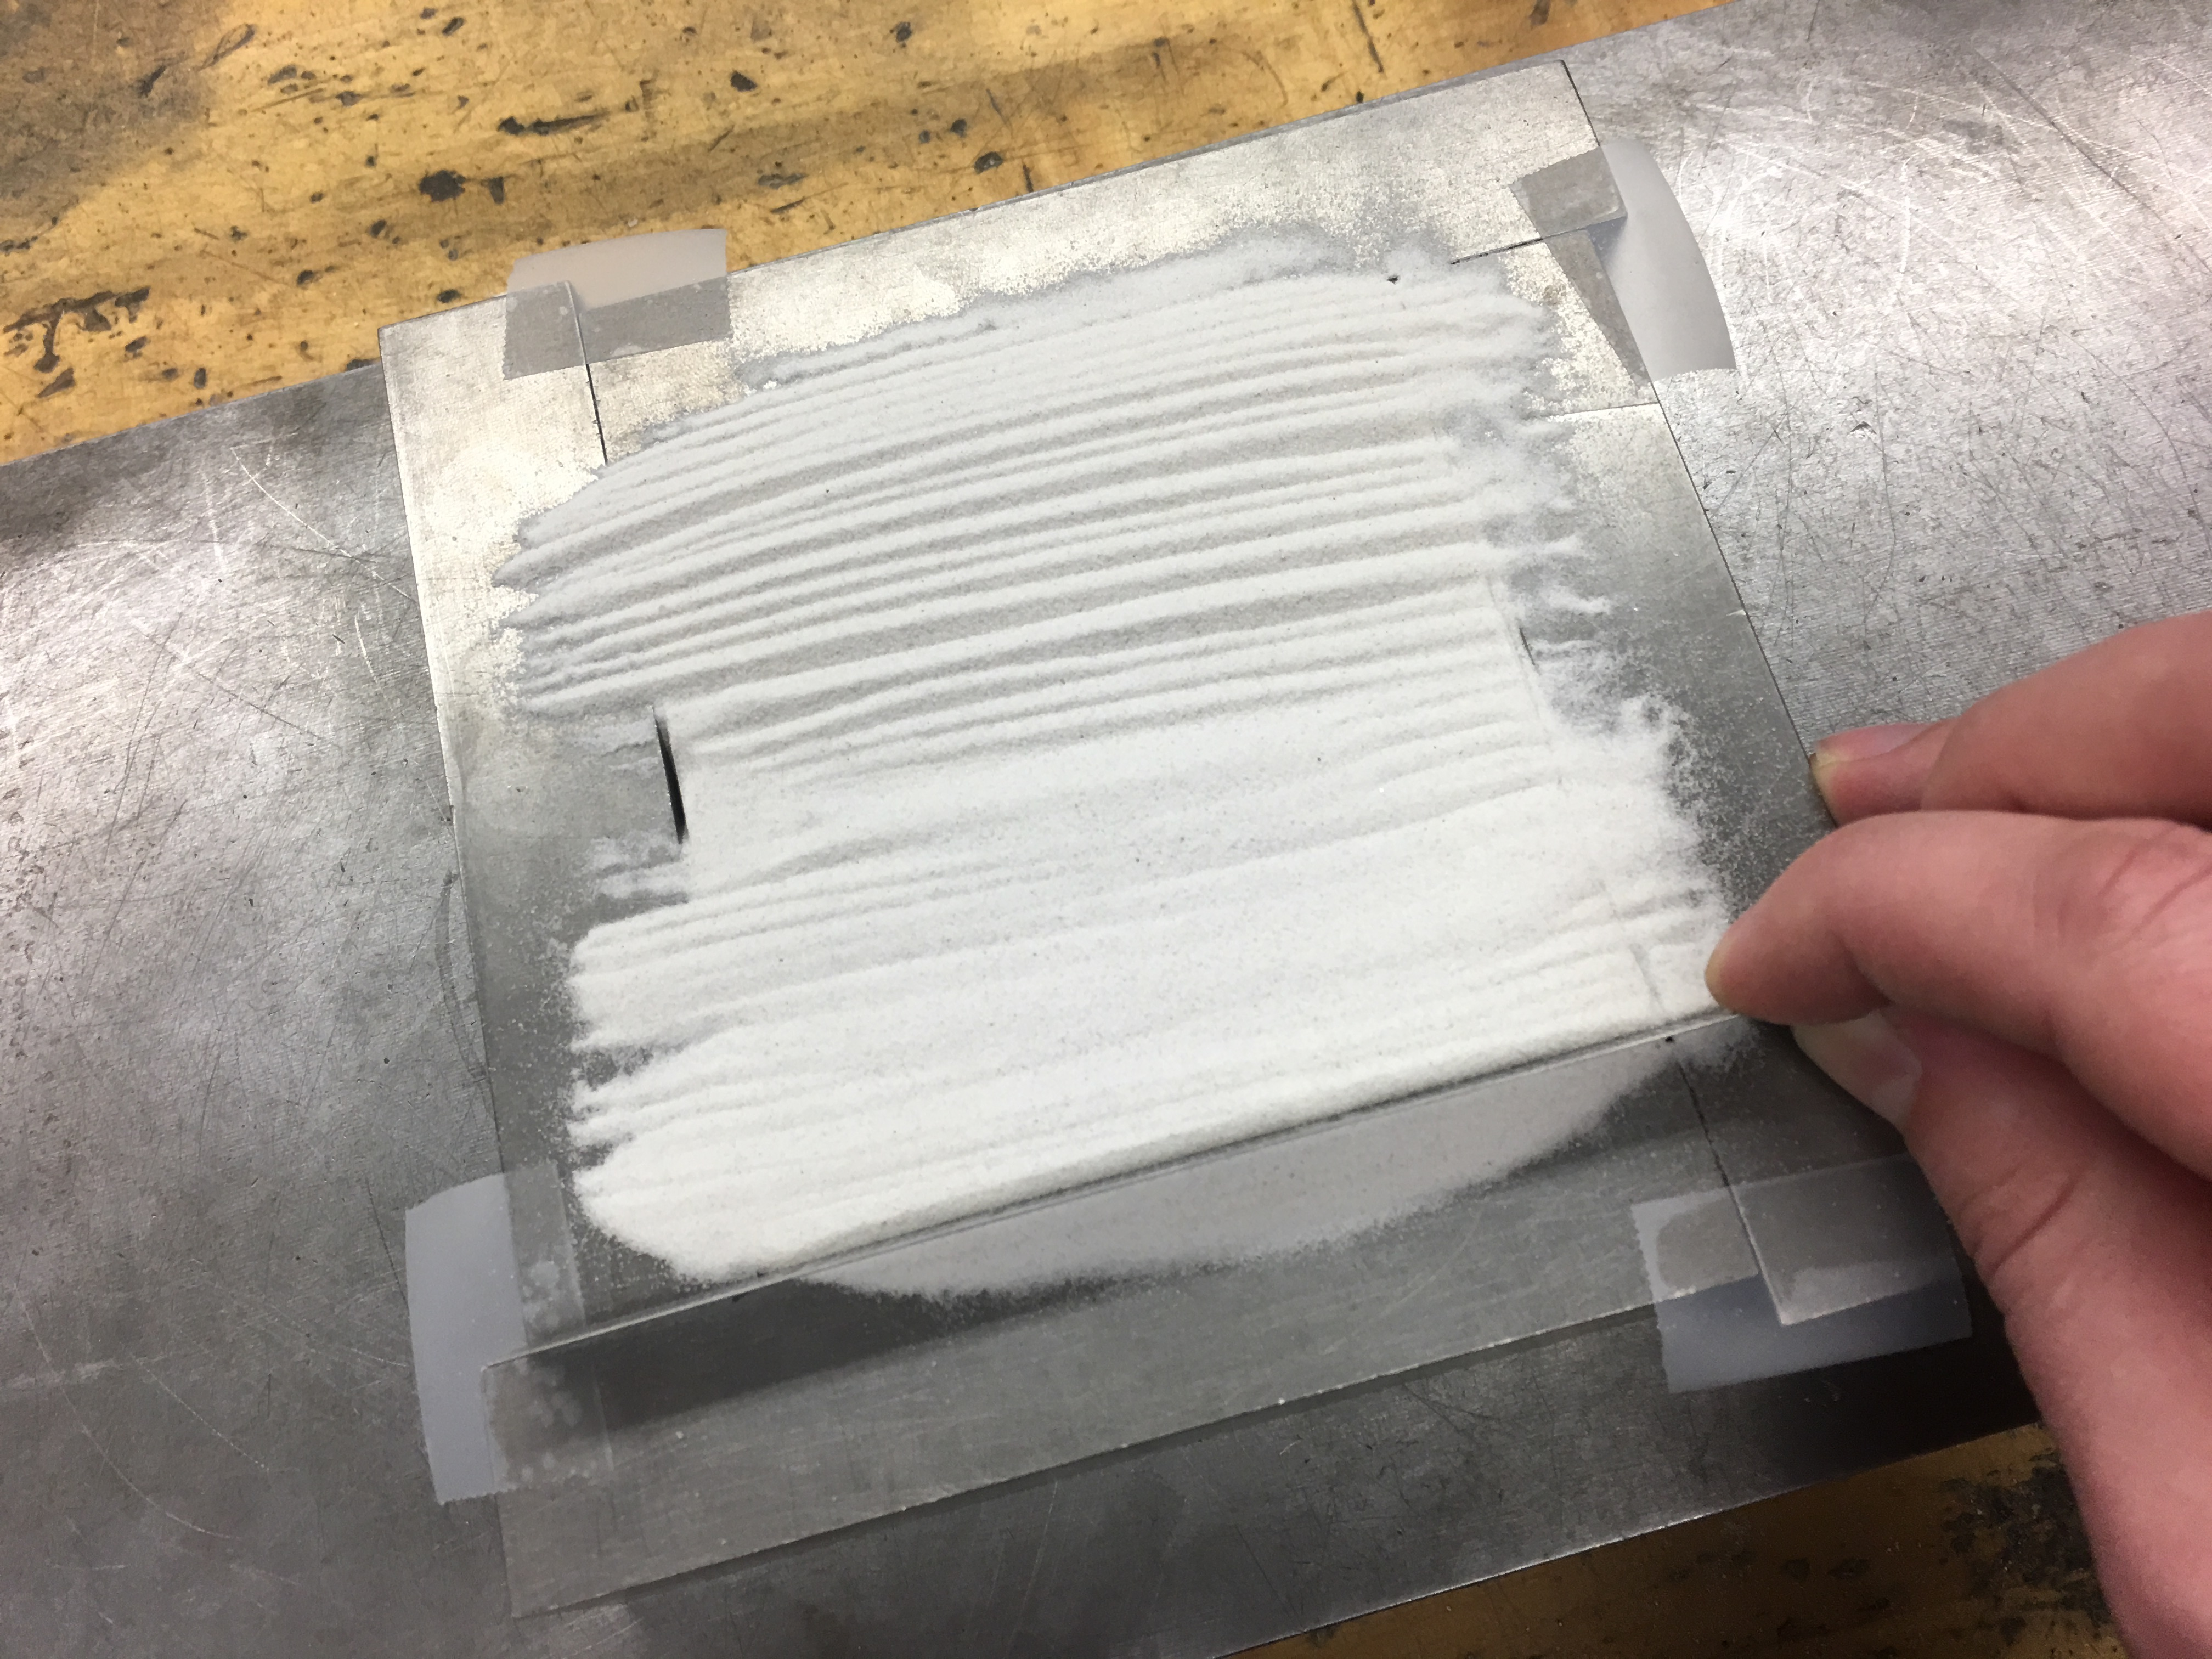
\includegraphics[width=0.7\textwidth]{appendix_sample_prep/dds_cutup_sample.jpg}
   	\caption{Using a sliding and chopping action, evenly distribute the sample material over the side block.}
  	\label{Fig:dds_cutup_sample}
\end{figure}
%% End Figure %%

%% Figure %%
\begin{figure}
	\centering
        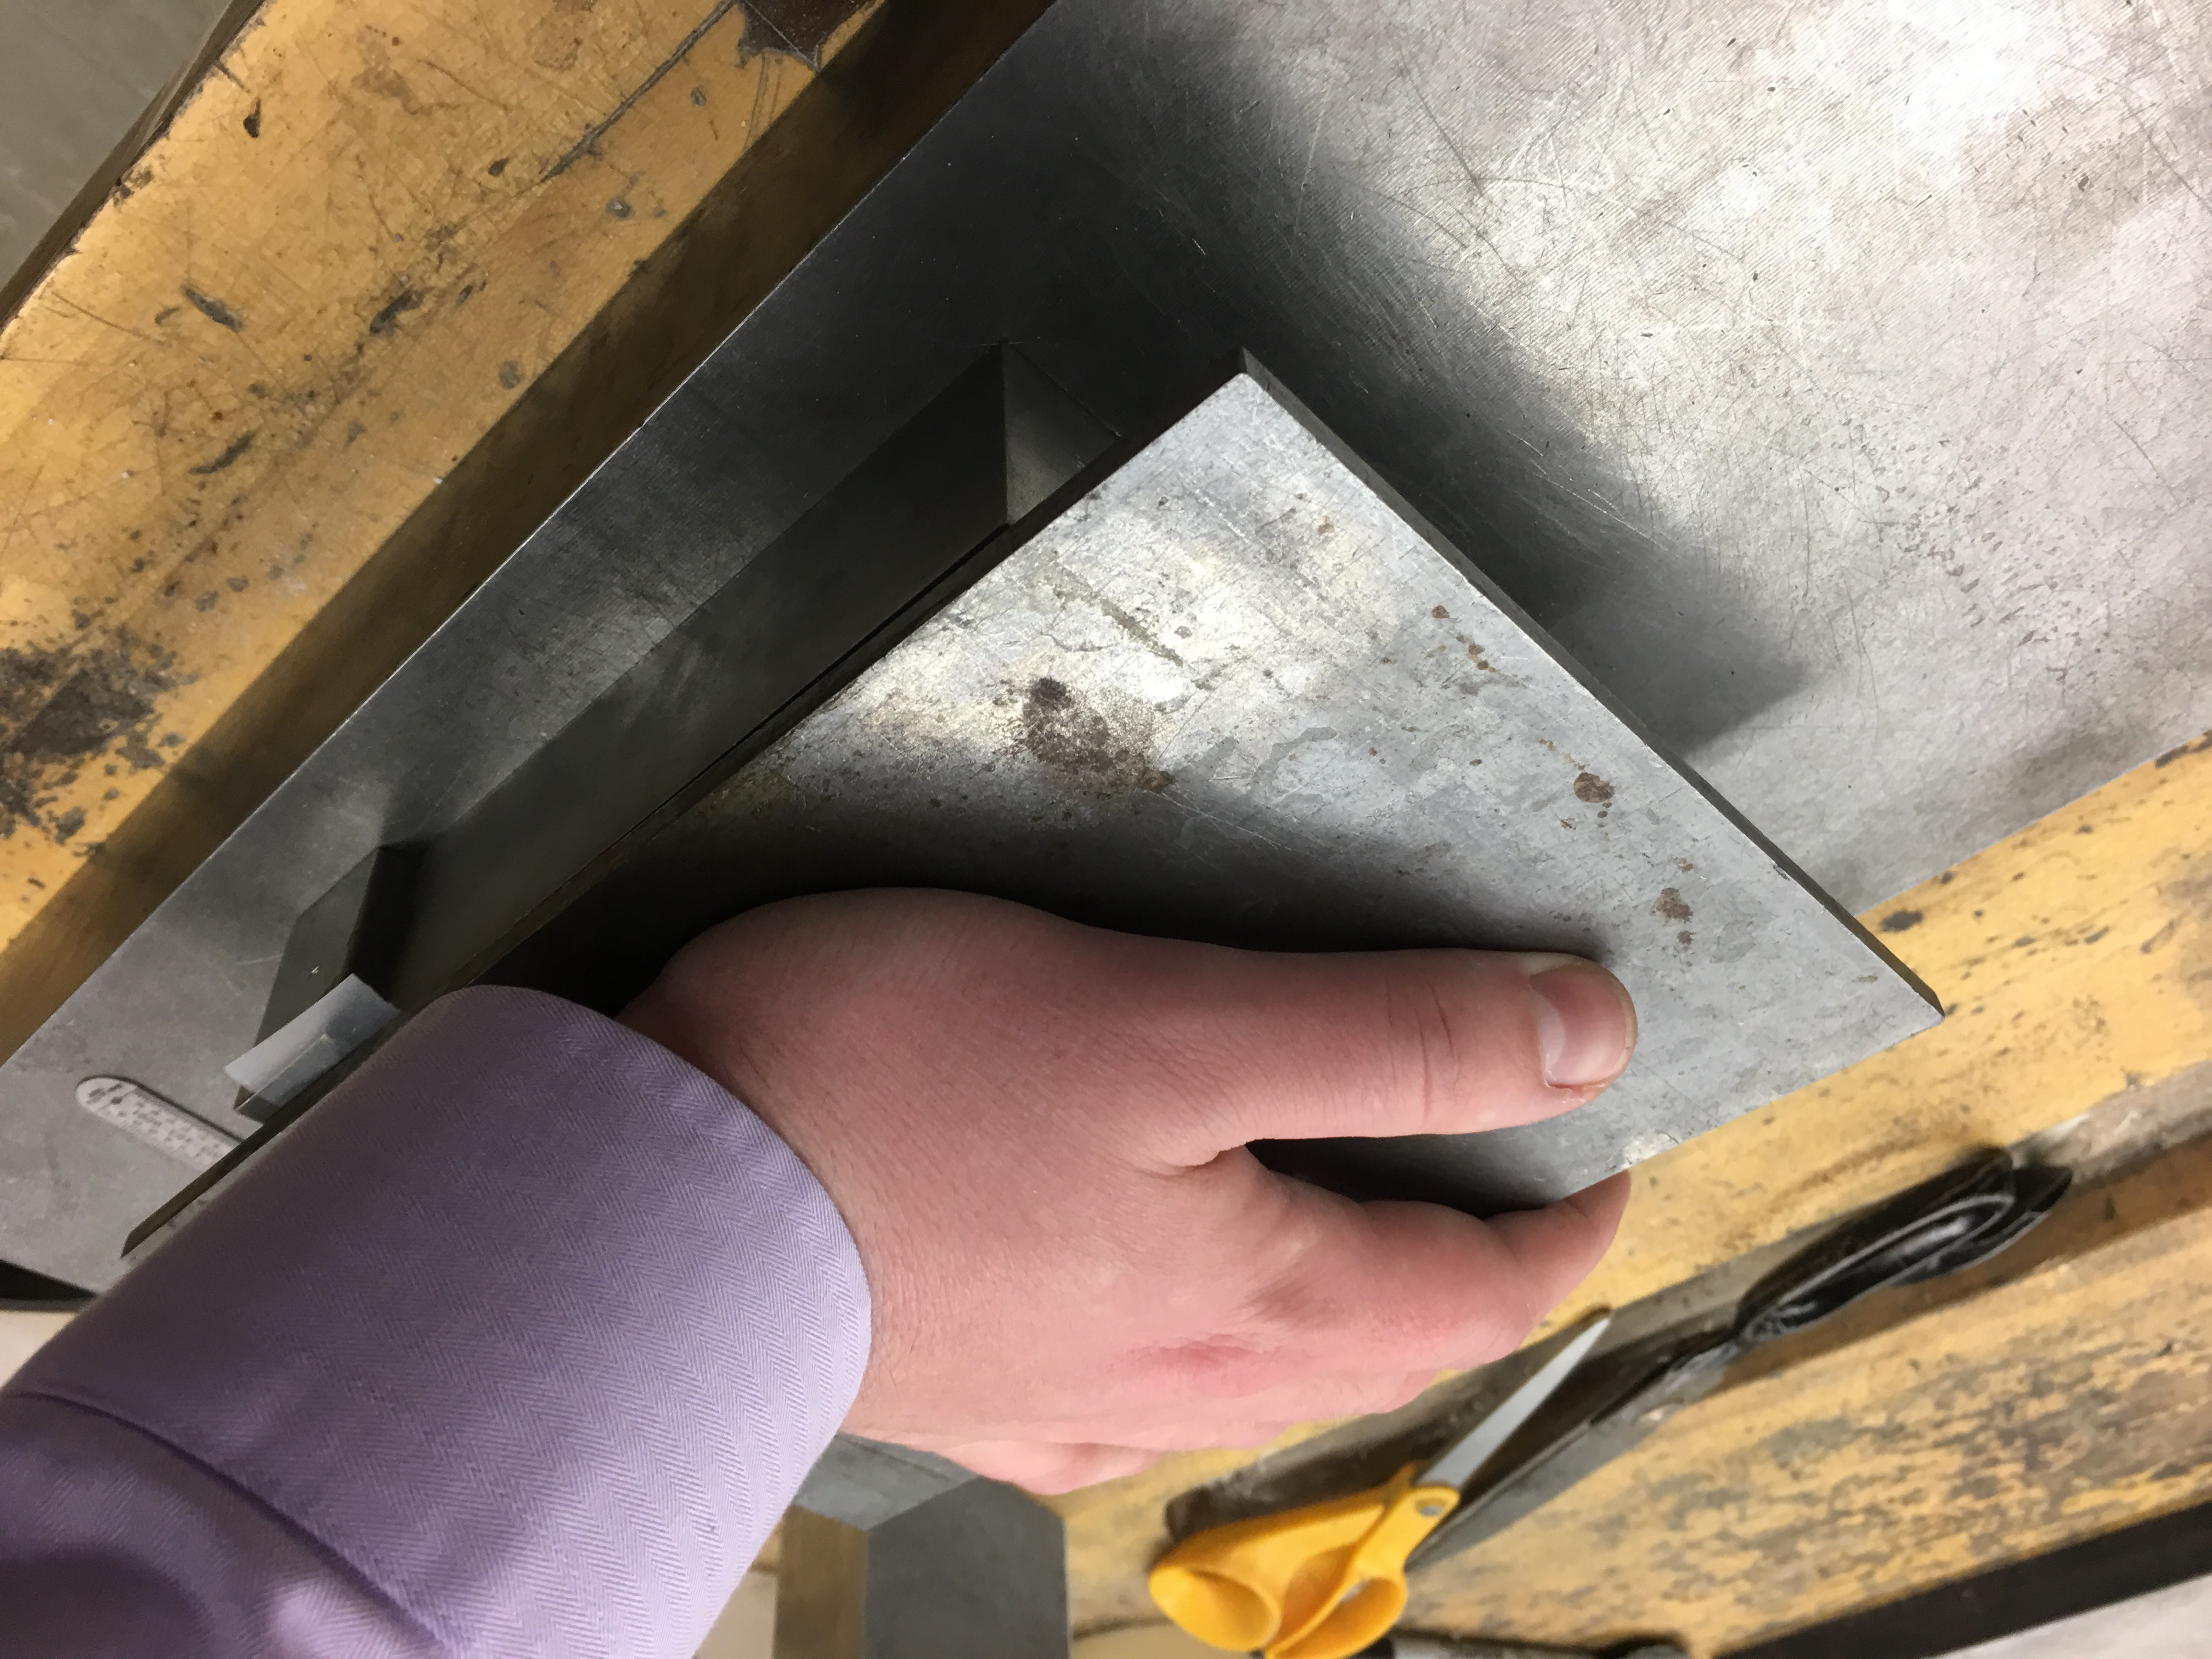
\includegraphics[width=0.7\textwidth]{appendix_sample_prep/dds_press_sample.jpg}
   	\caption{Firmly compress the sample to ensure a good granular packing.}
  	\label{Fig:dds_press_sample}
\end{figure}
%% End Figure %%

\clearpage

%% Figure %%
\begin{figure}
	\centering
        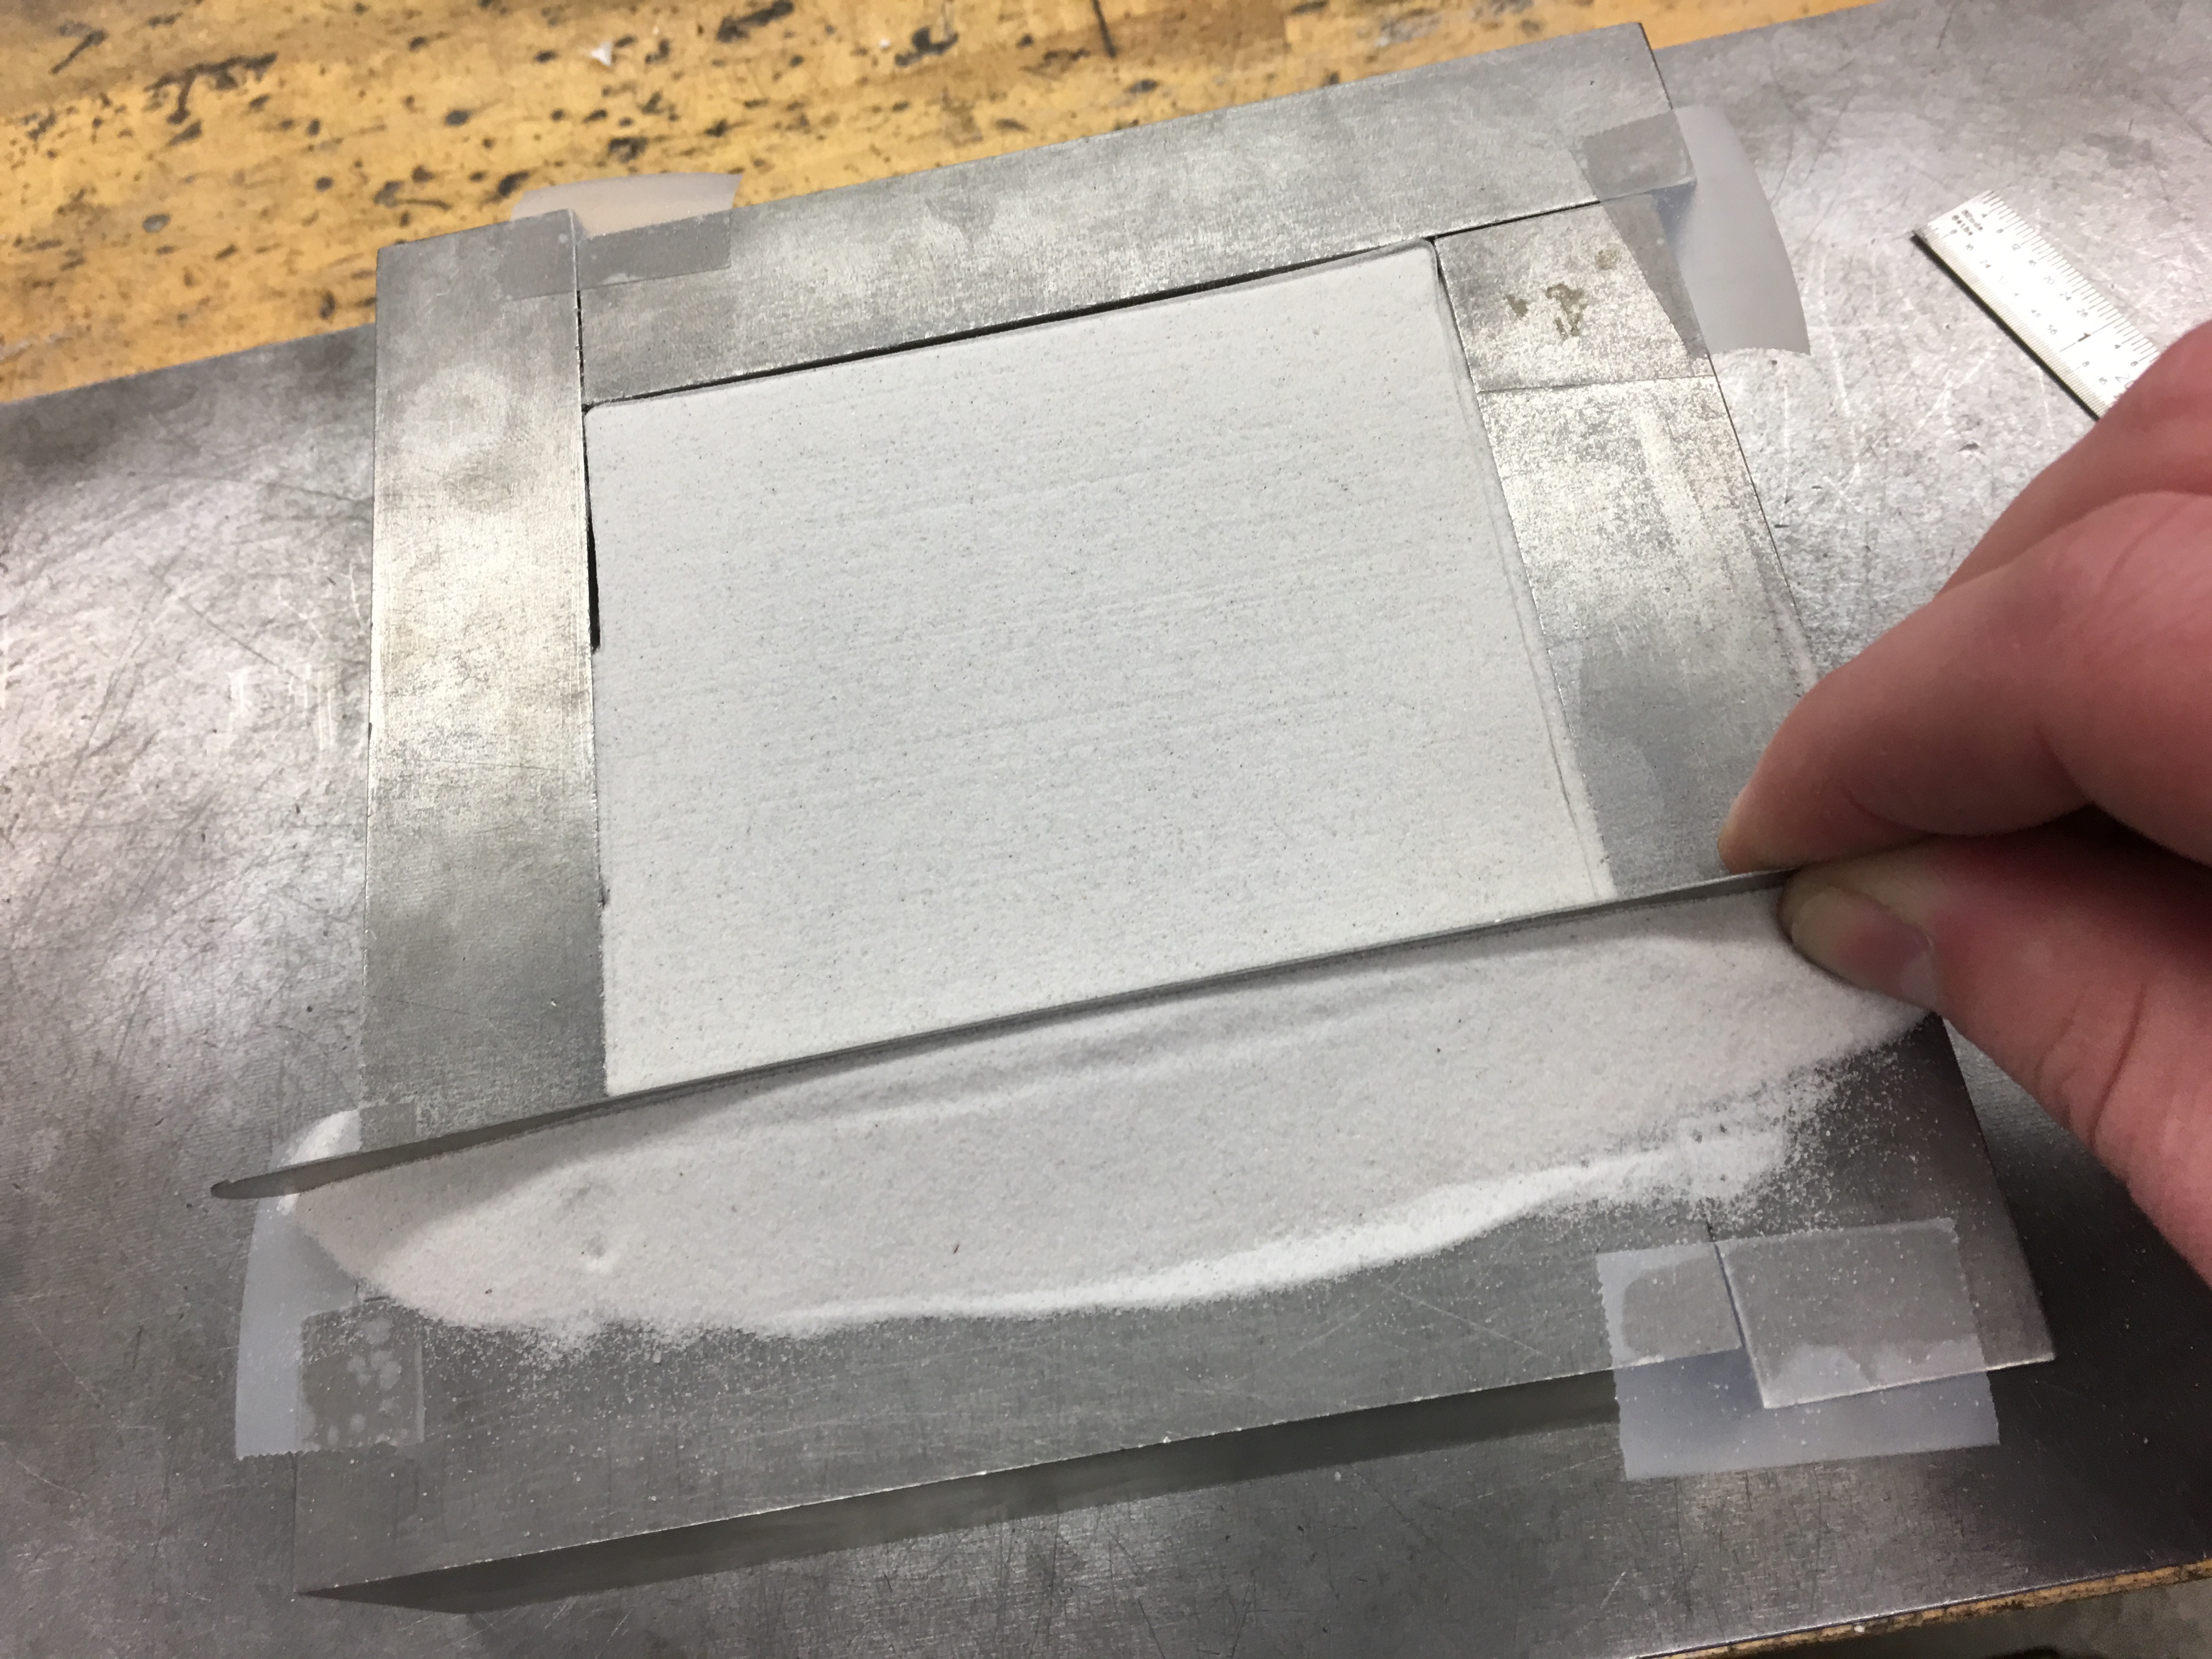
\includegraphics[width=0.7\textwidth]{appendix_sample_prep/dds_level_sample.jpg}
   	\caption{Drag the steel rule over the sample to flatten the layer.}
  	\label{Fig:dds_level_sample}
\end{figure}
%% End Figure %%

%% Figure %%
\begin{figure}
	\centering
        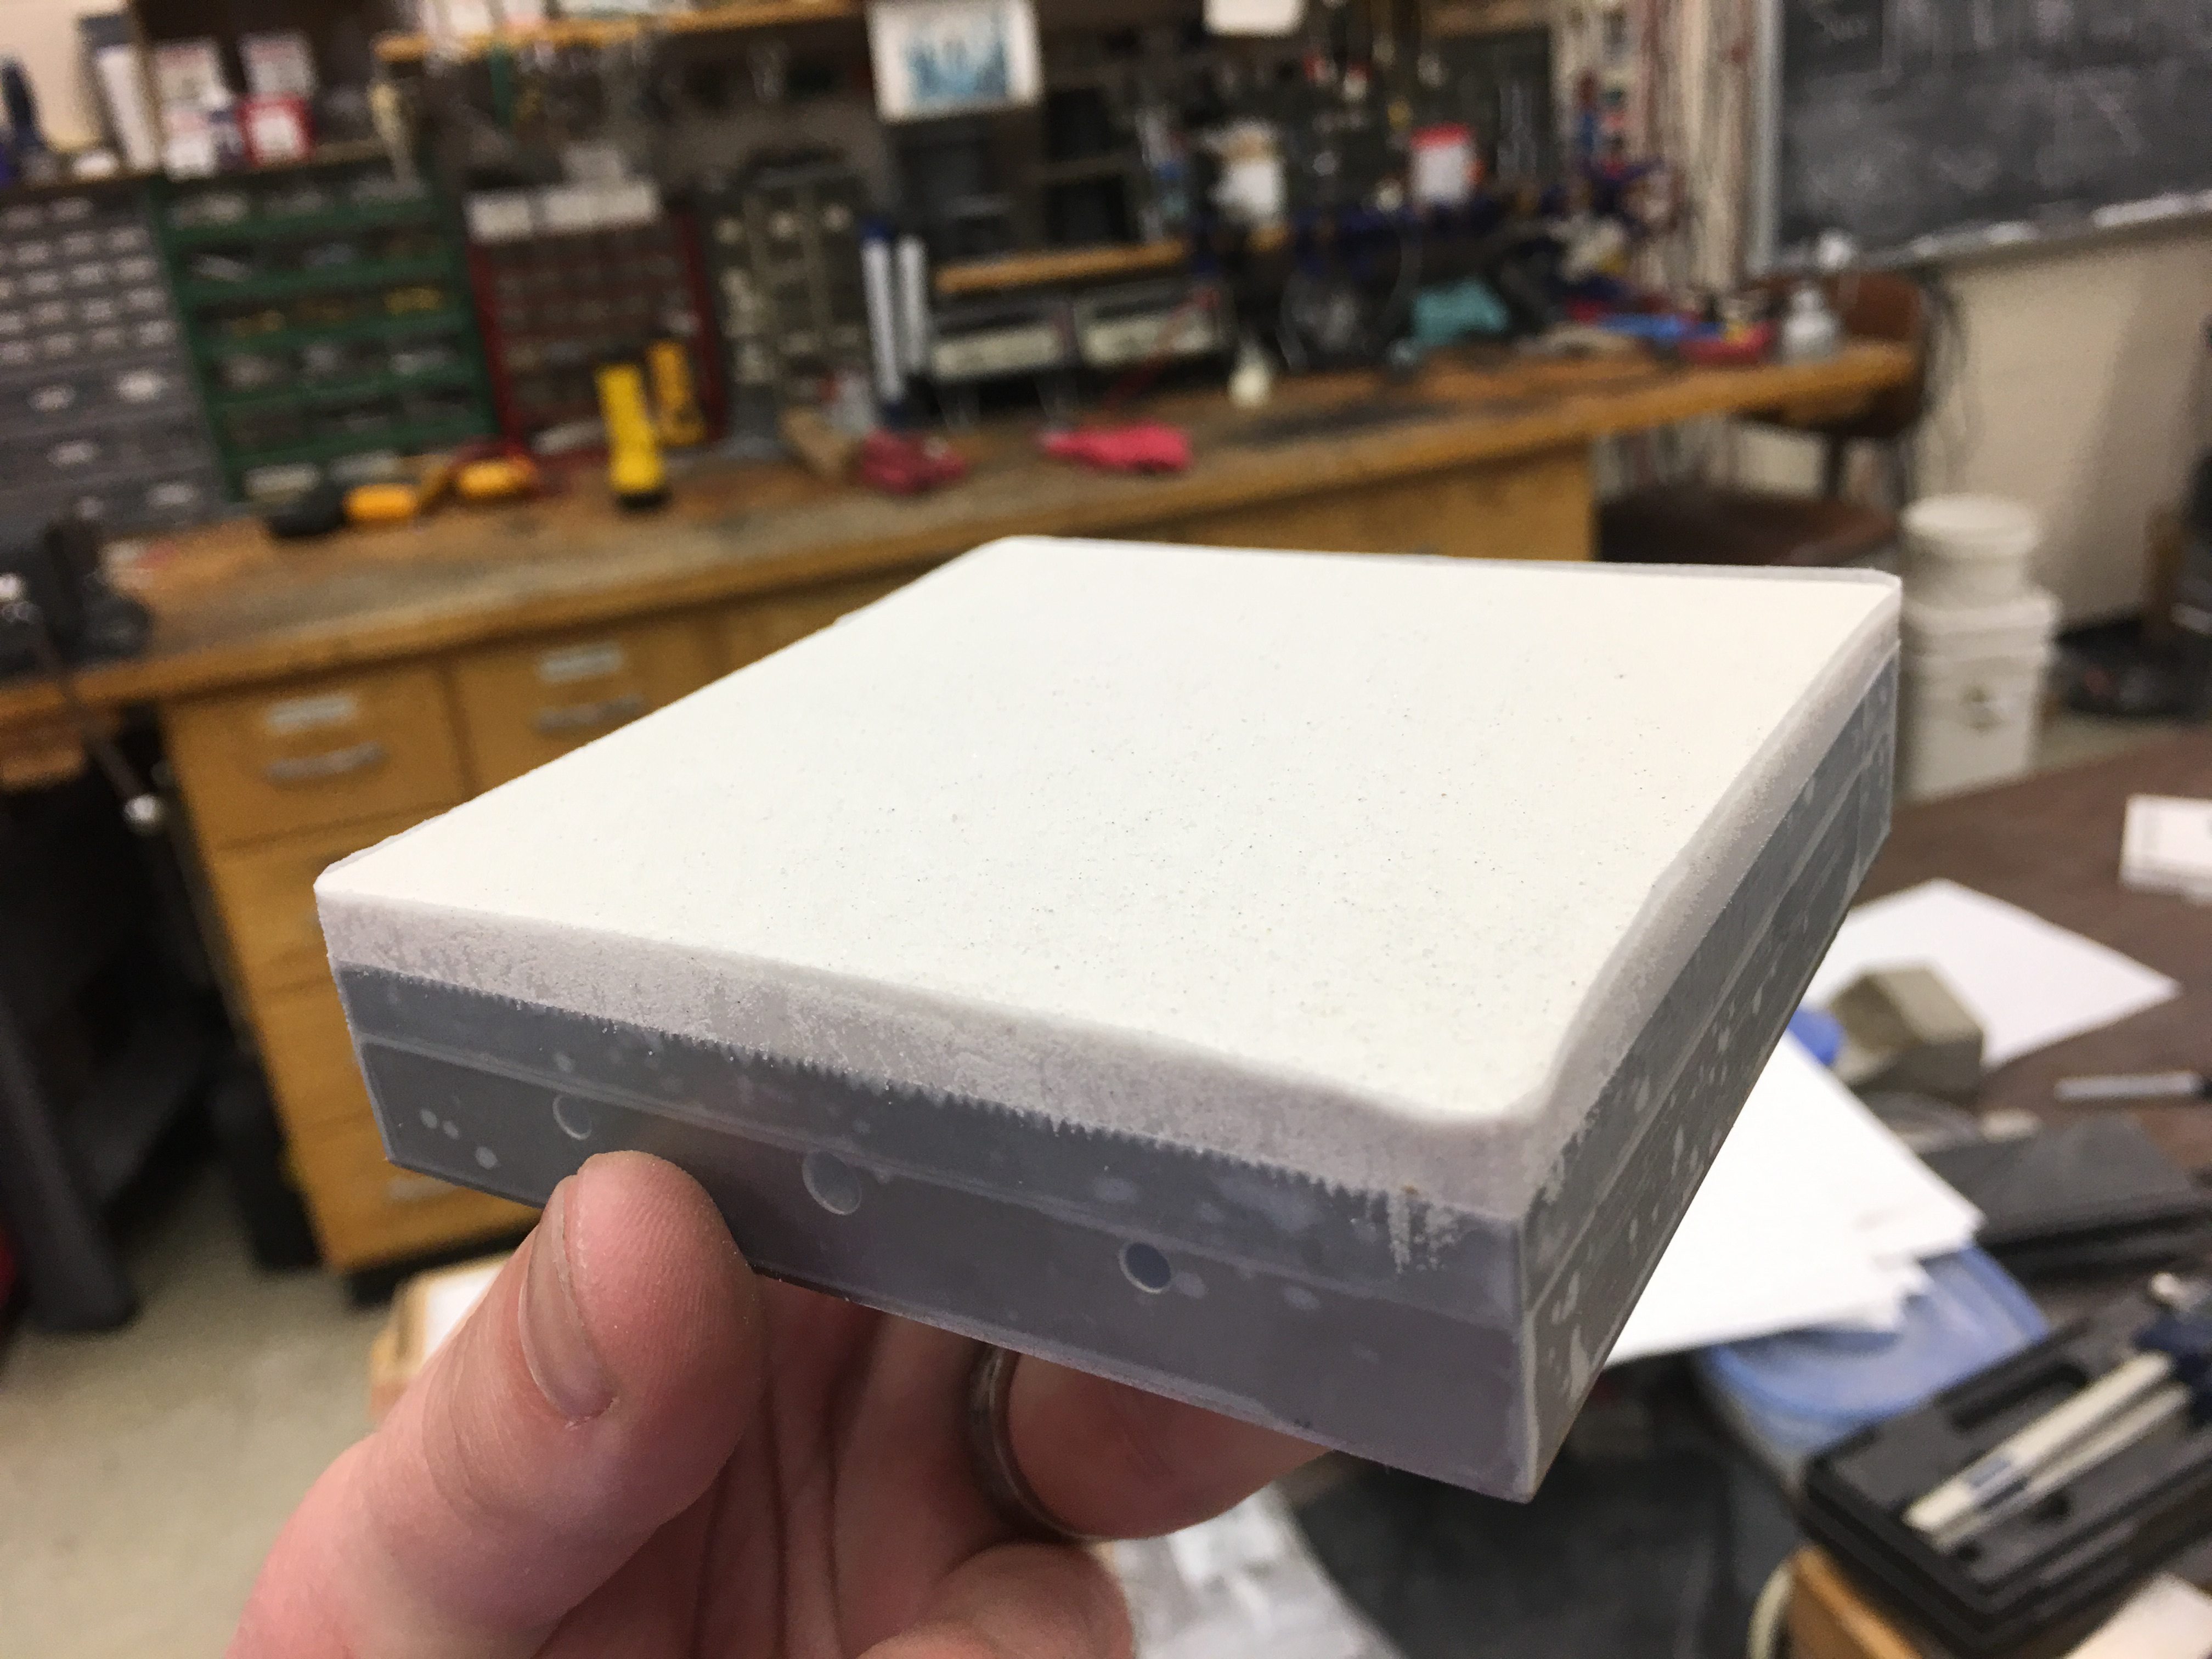
\includegraphics[width=0.7\textwidth]{appendix_sample_prep/dds_finished_sideblock.jpg}
   	\caption{A completed side block ready to be weighed and assembled.}
  	\label{Fig:dds_finished_sideblock}
\end{figure}
%% End Figure %%

%% Figure %%
\begin{figure}
	\centering
        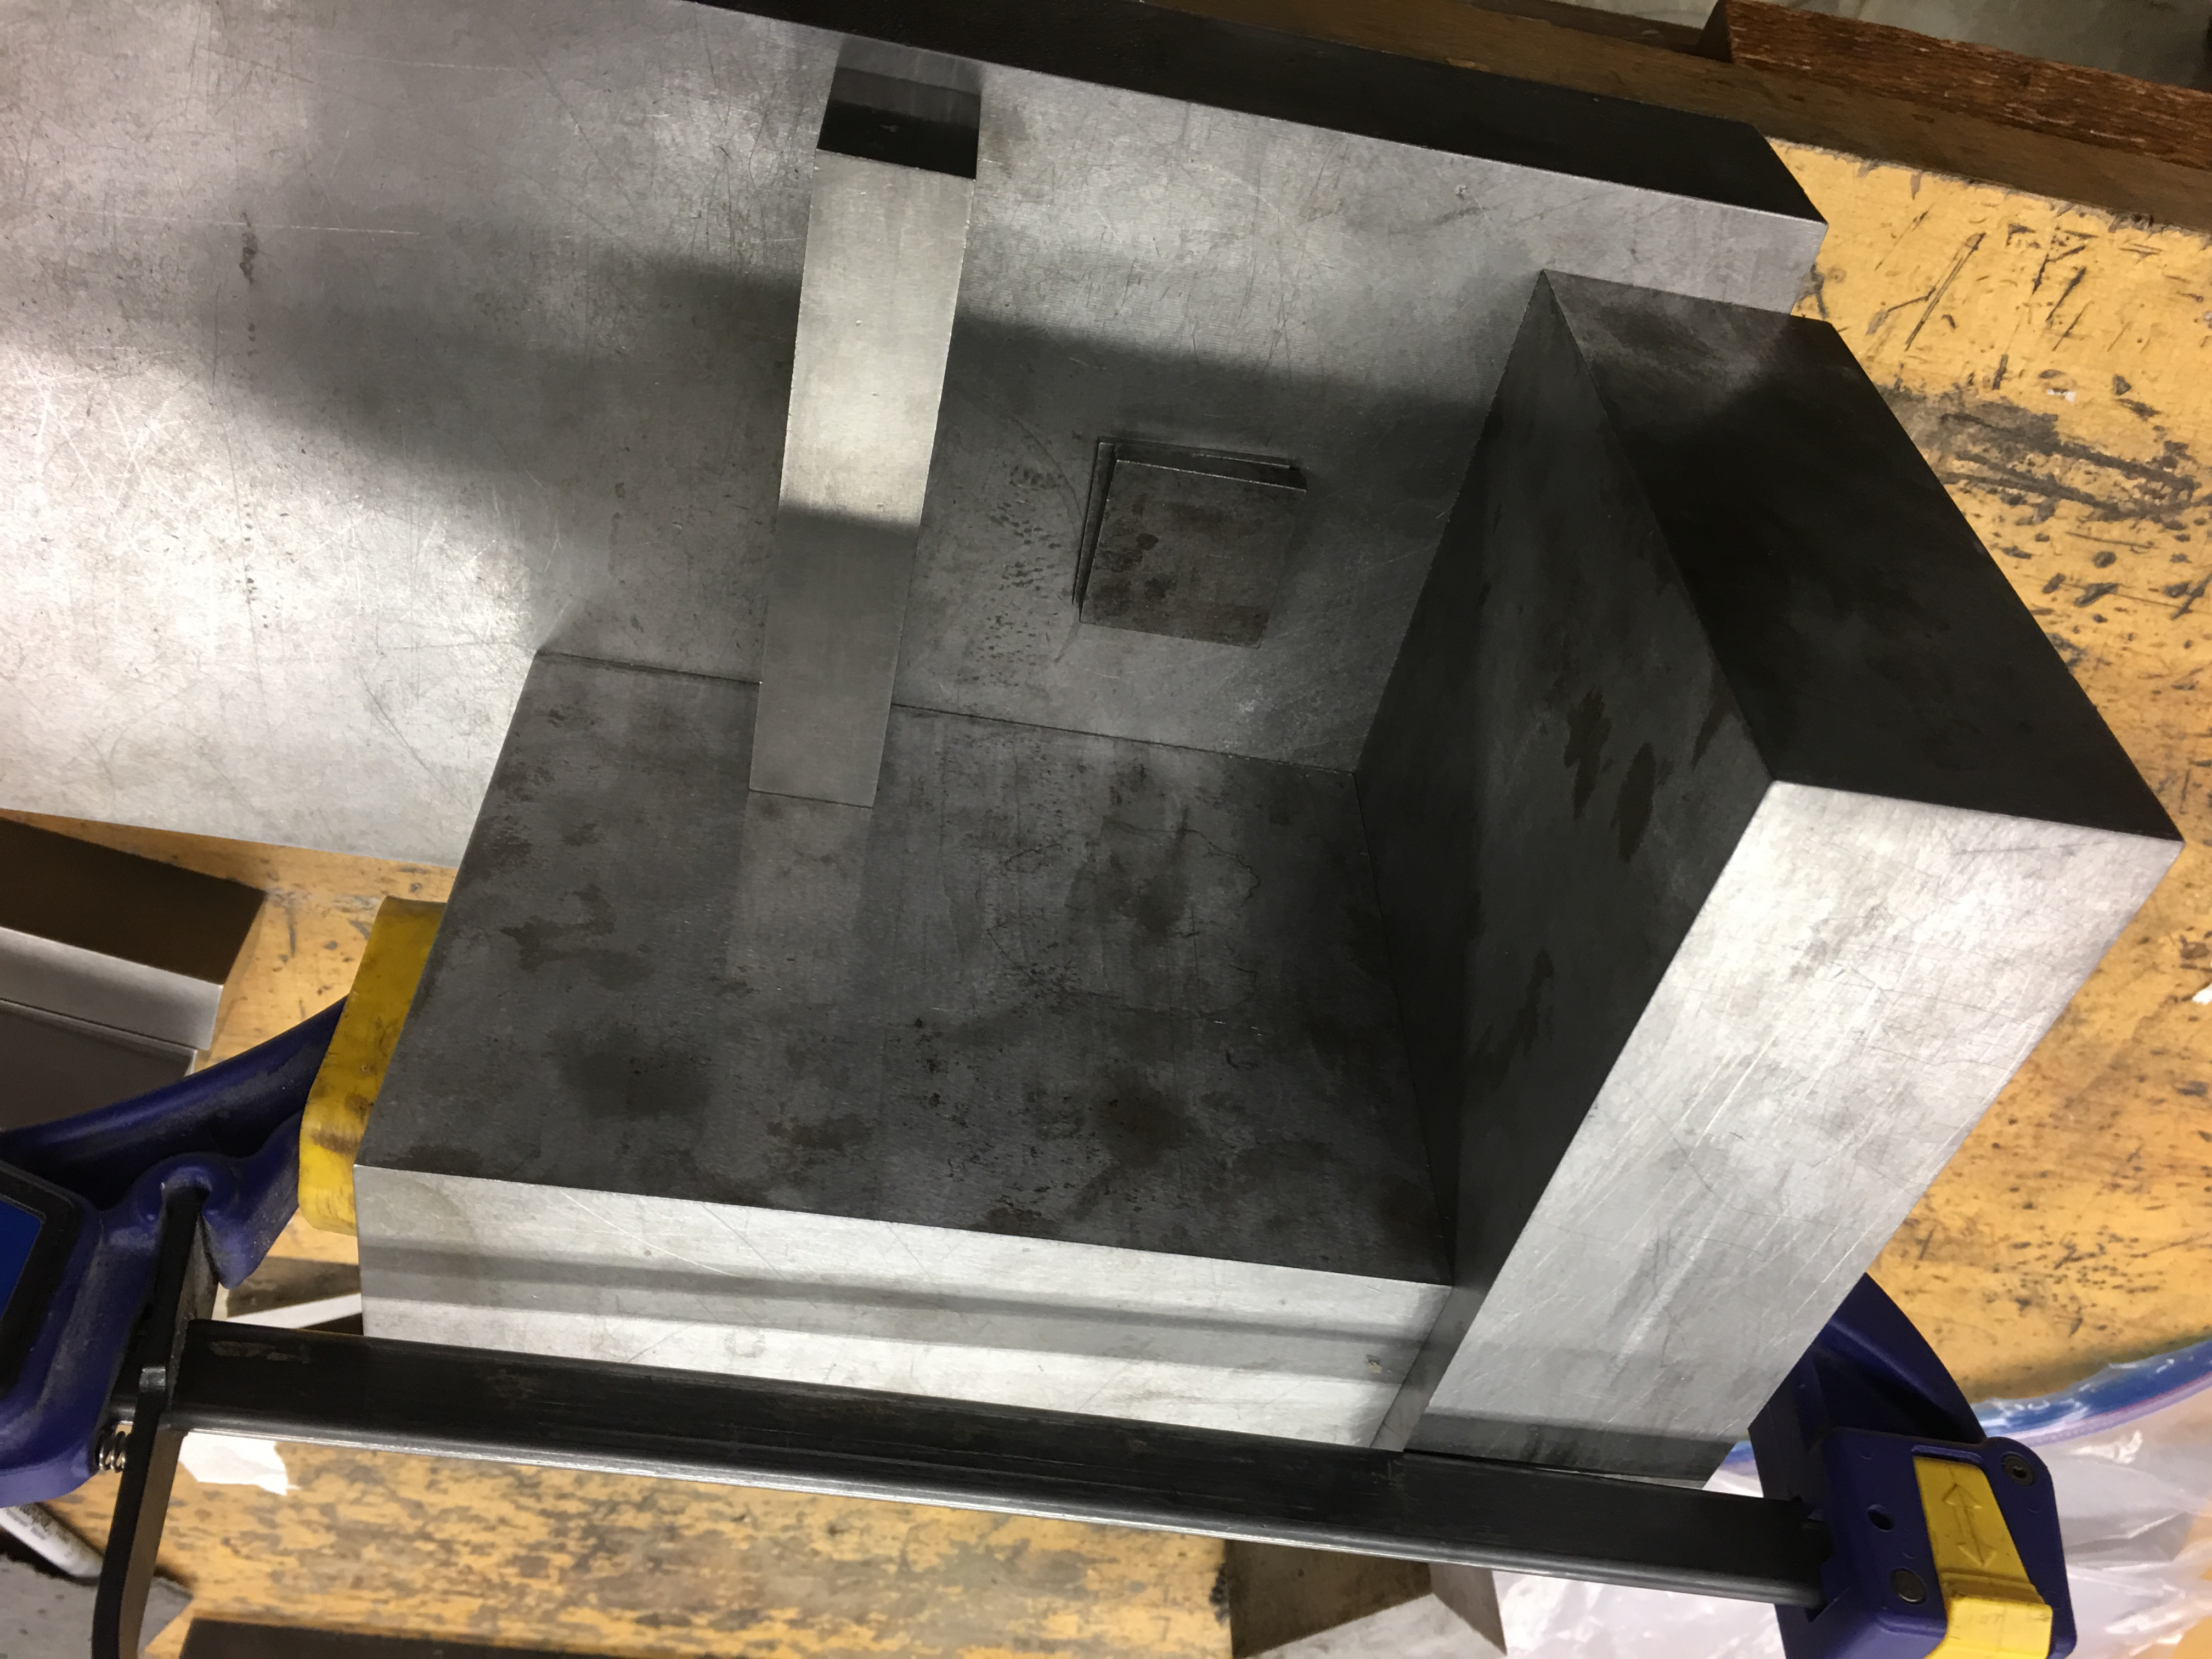
\includegraphics[width=0.7\textwidth]{appendix_sample_prep/dds_ell_jig.jpg}
   	\caption{Setup the jig for assembling the side and center blocks into the complete sample assembly.}
  	\label{Fig:dds_ell_jig}
\end{figure}
%% End Figure %%

%% Figure %%
\begin{figure}
	\centering
        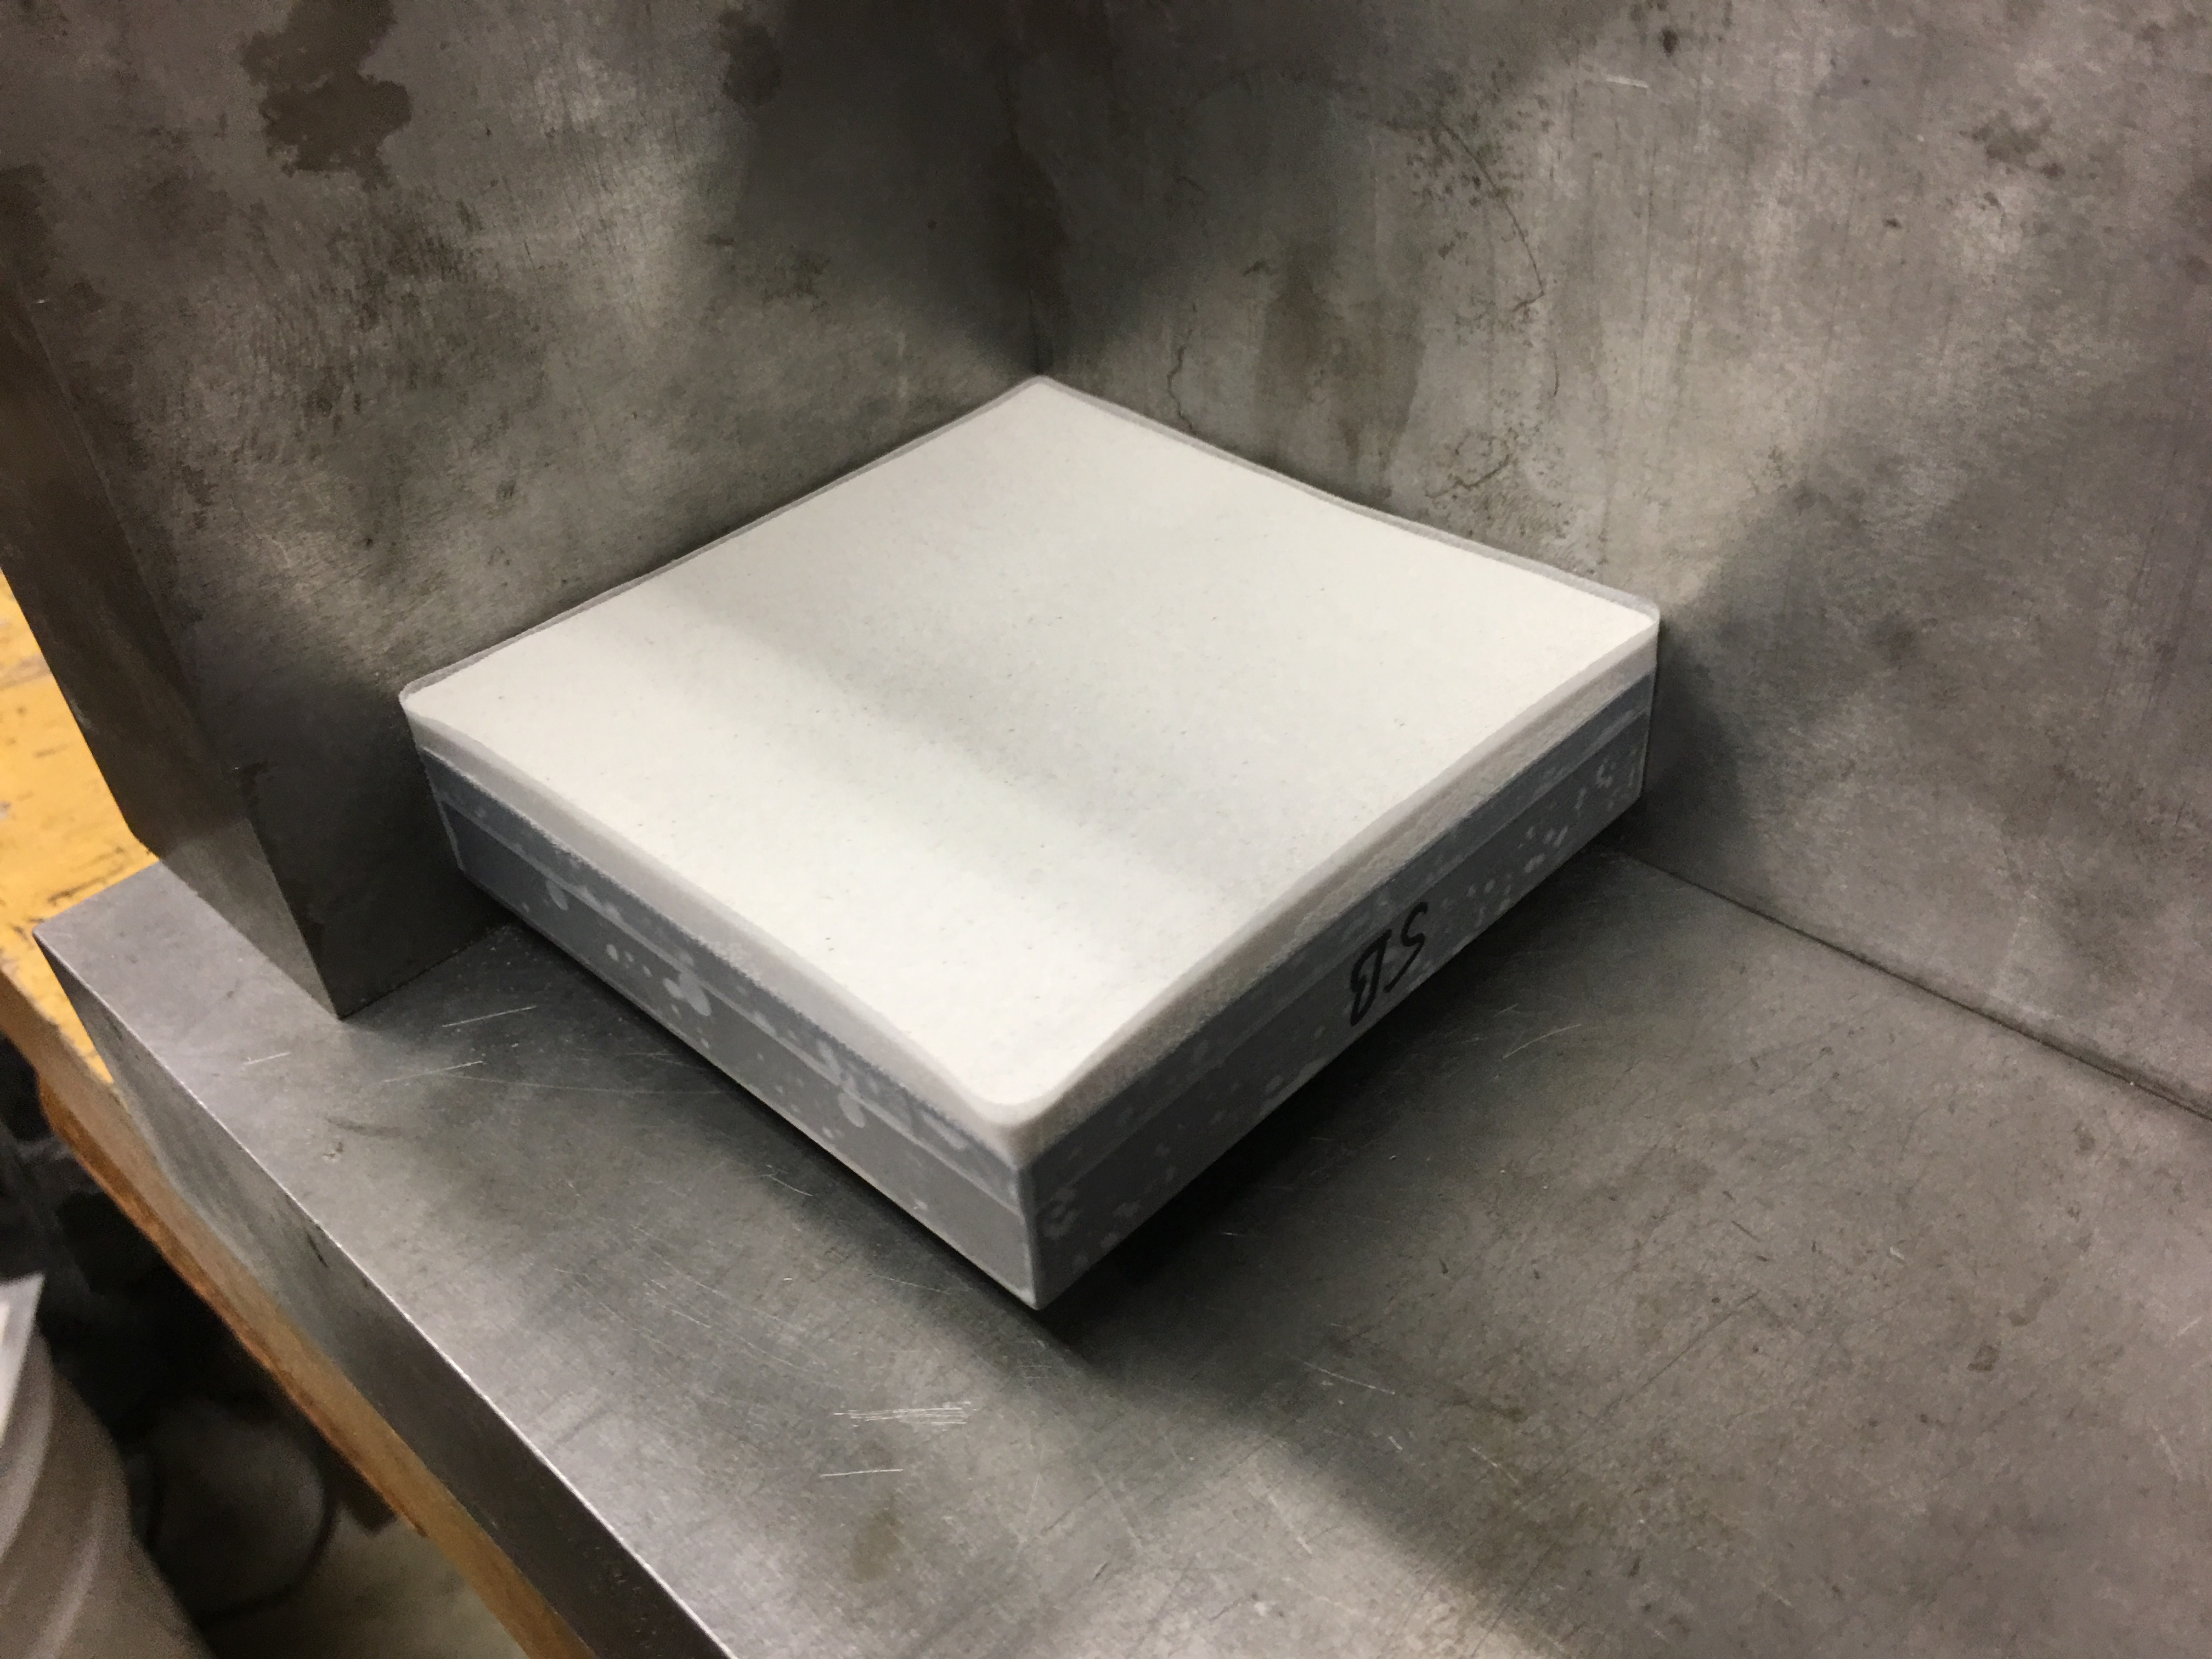
\includegraphics[width=0.7\textwidth]{appendix_sample_prep/dds_sideblock_jig.jpg}
   	\caption{Place the sideblock into the jig with the side shield mounts facing towards you.}
  	\label{Fig:dds_sideblock_jig}
\end{figure}
%% End Figure %%

\clearpage

%% Figure %%
\begin{figure}
	\centering
        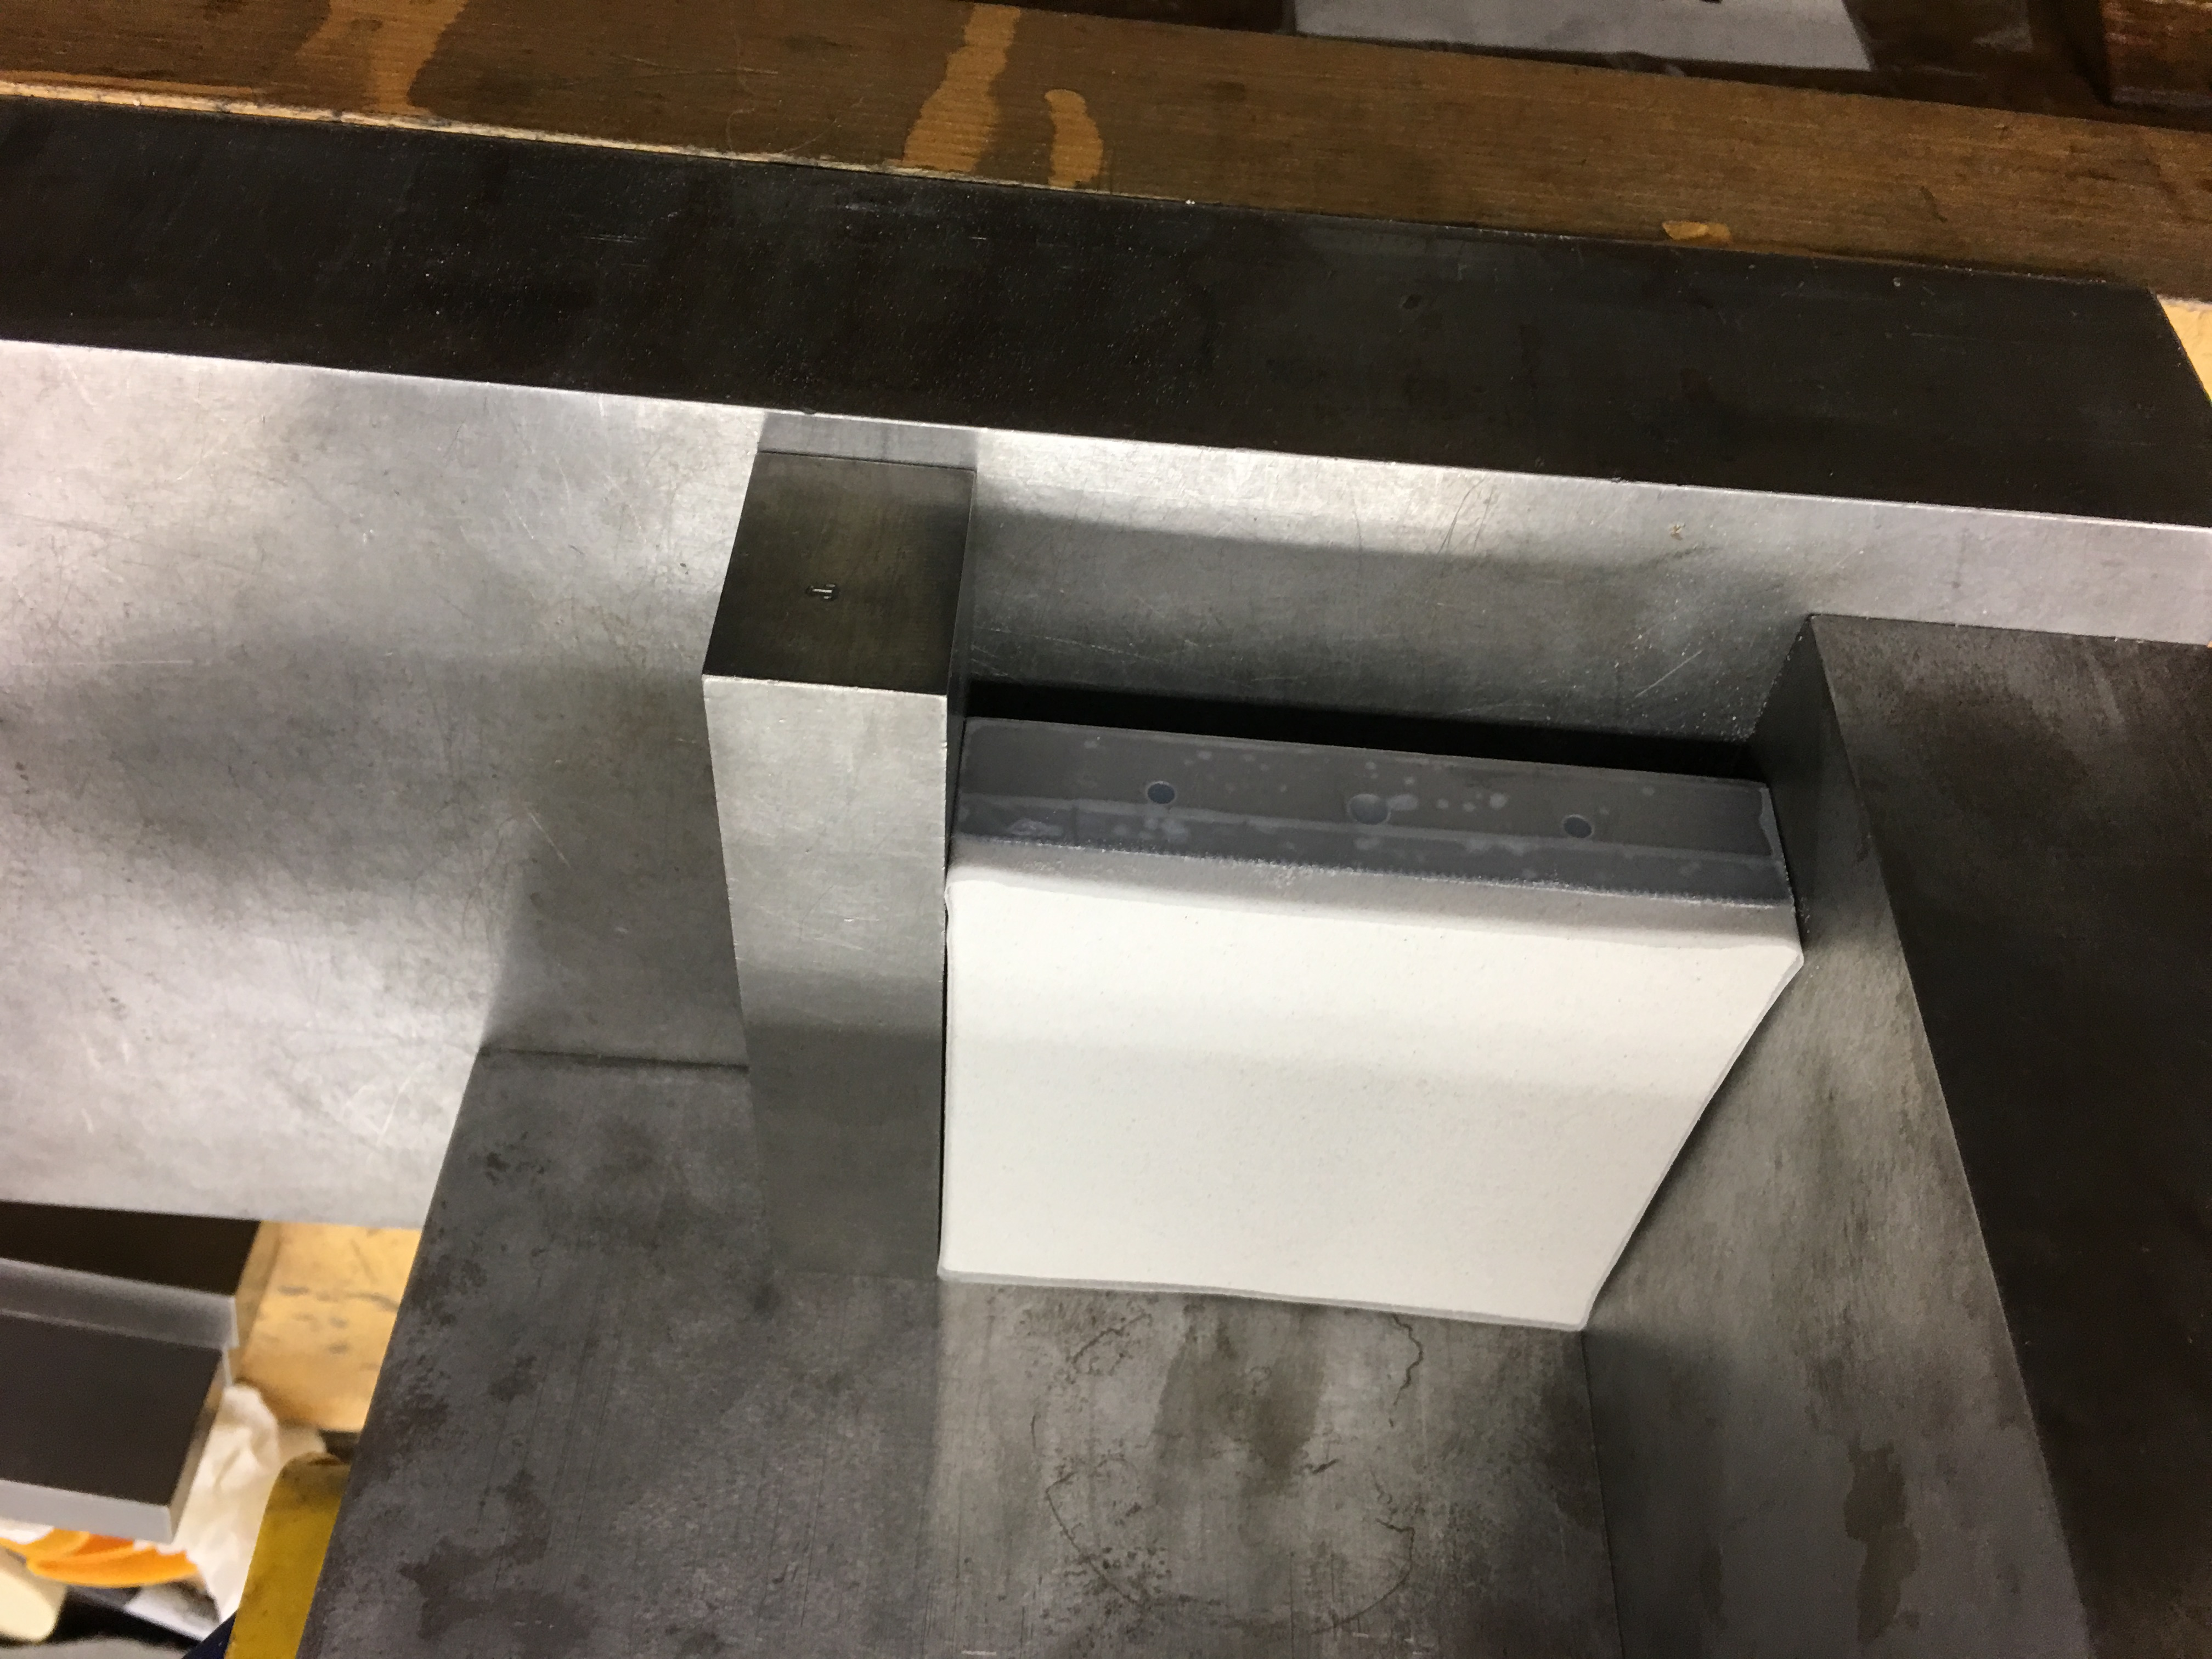
\includegraphics[width=0.7\textwidth]{appendix_sample_prep/dds_sideblock_jig_2.jpg}
   	\caption{Place a spacer at the top of the side block to help support the center block's weight.}
  	\label{Fig:dds_sideblock_jig_2}
\end{figure}
%% End Figure %%

%% Figure %%
\begin{figure}
	\centering
        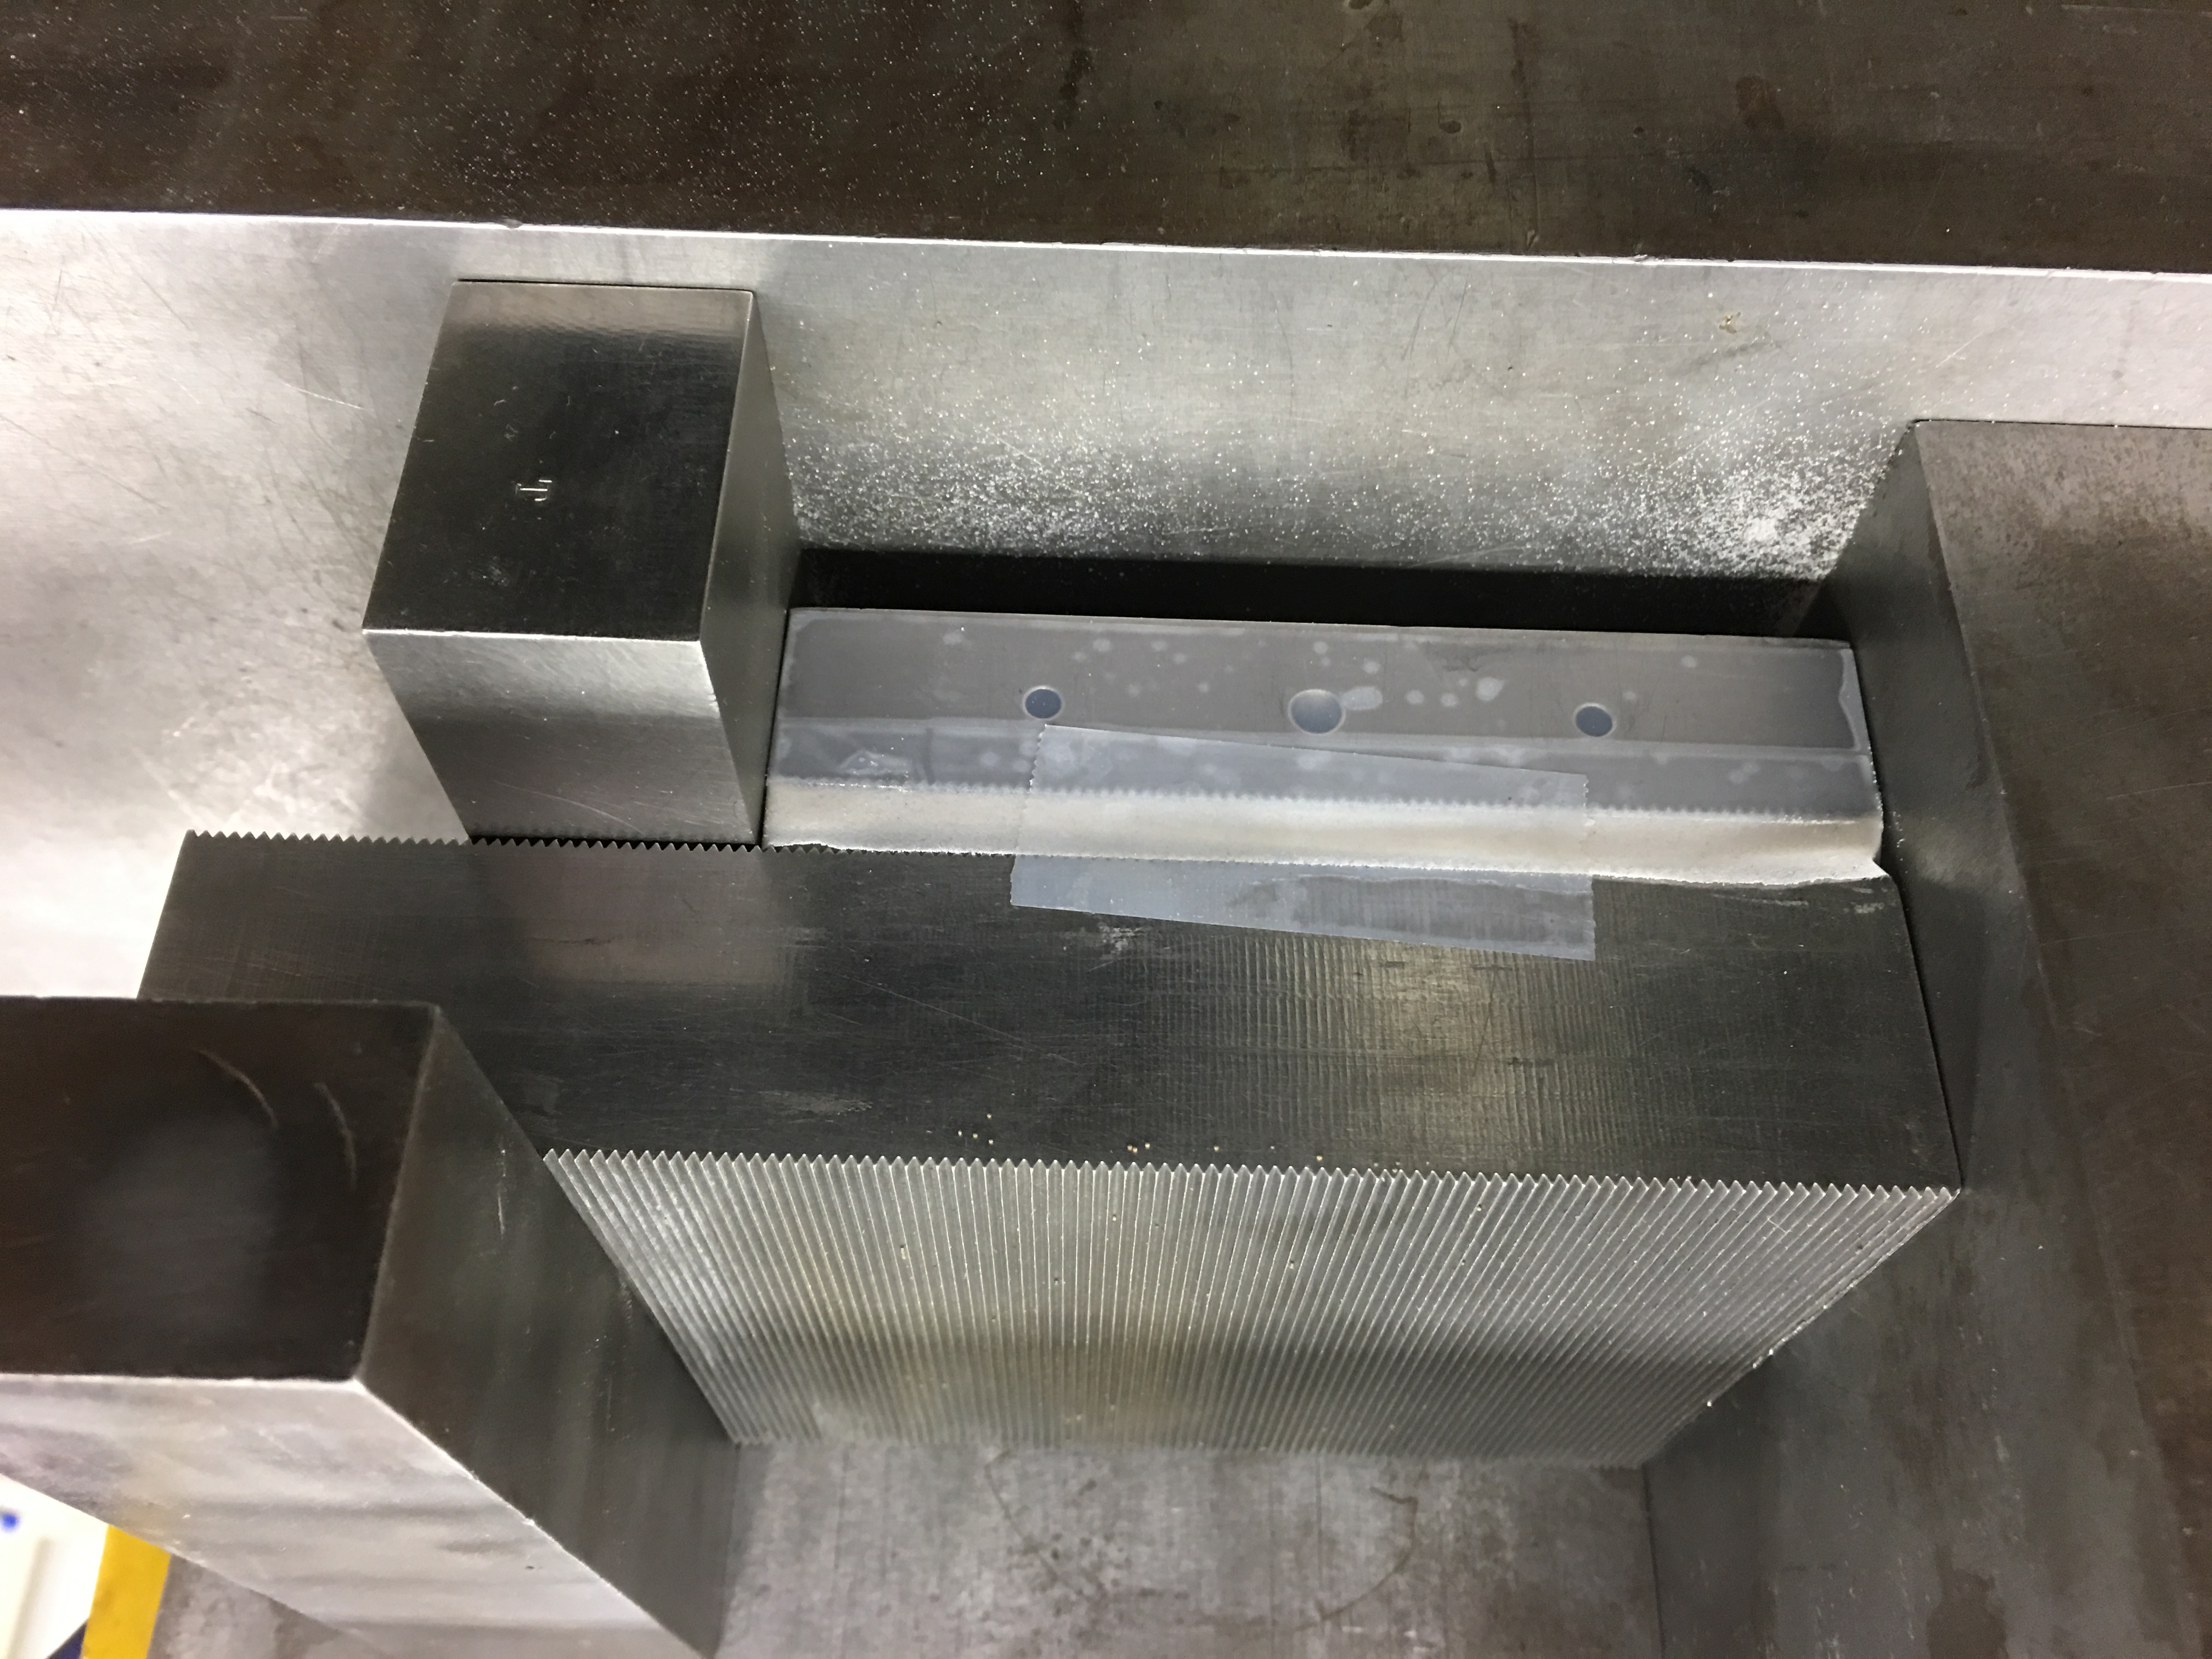
\includegraphics[width=0.7\textwidth]{appendix_sample_prep/dds_centerblock_jig.jpg}
   	\caption{Place the center block on and secure it with small strips of tape. Note the counterweight block on top of the center block.}
  	\label{Fig:dds_centerblock_jig}
\end{figure}
%% End Figure %%

%% Figure %%
\begin{figure}
	\centering
        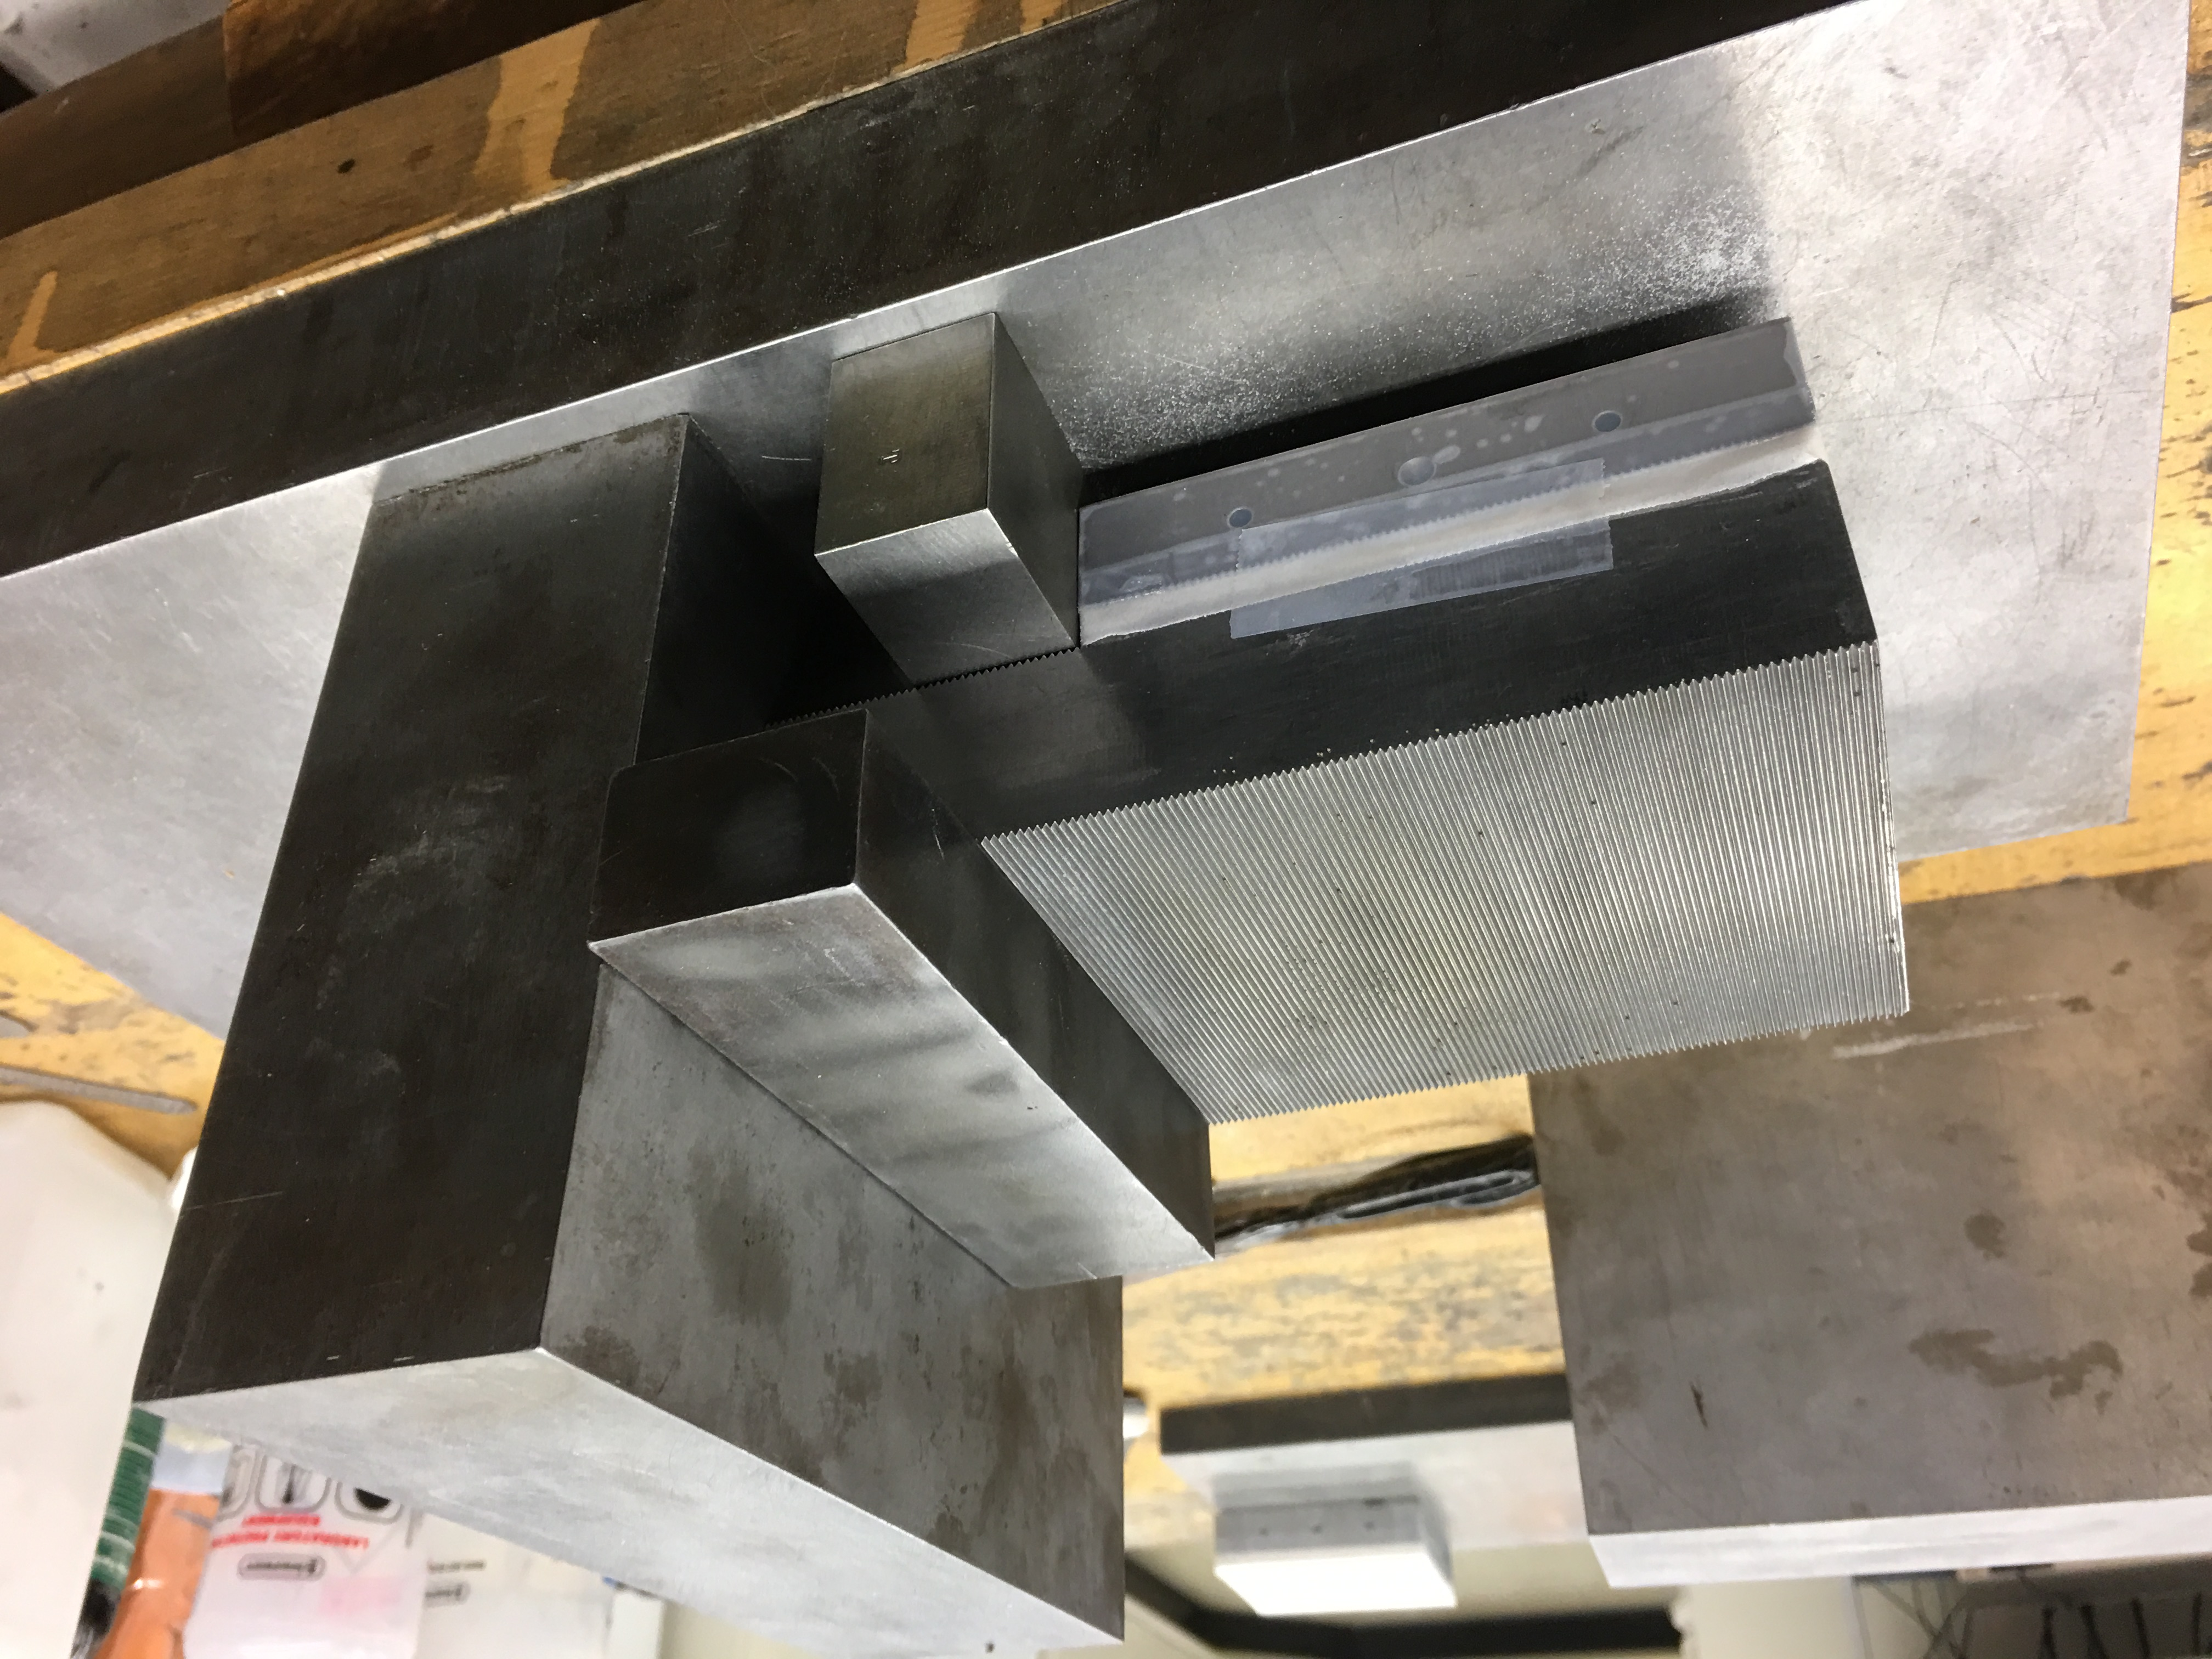
\includegraphics[width=0.7\textwidth]{appendix_sample_prep/dds_move_block.jpg}
   	\caption{Rearrange the jig so that the sample can be taped without moving.}
  	\label{Fig:dds_move_block}
\end{figure}
%% End Figure %%

%% Figure %%
\begin{figure}
	\centering
        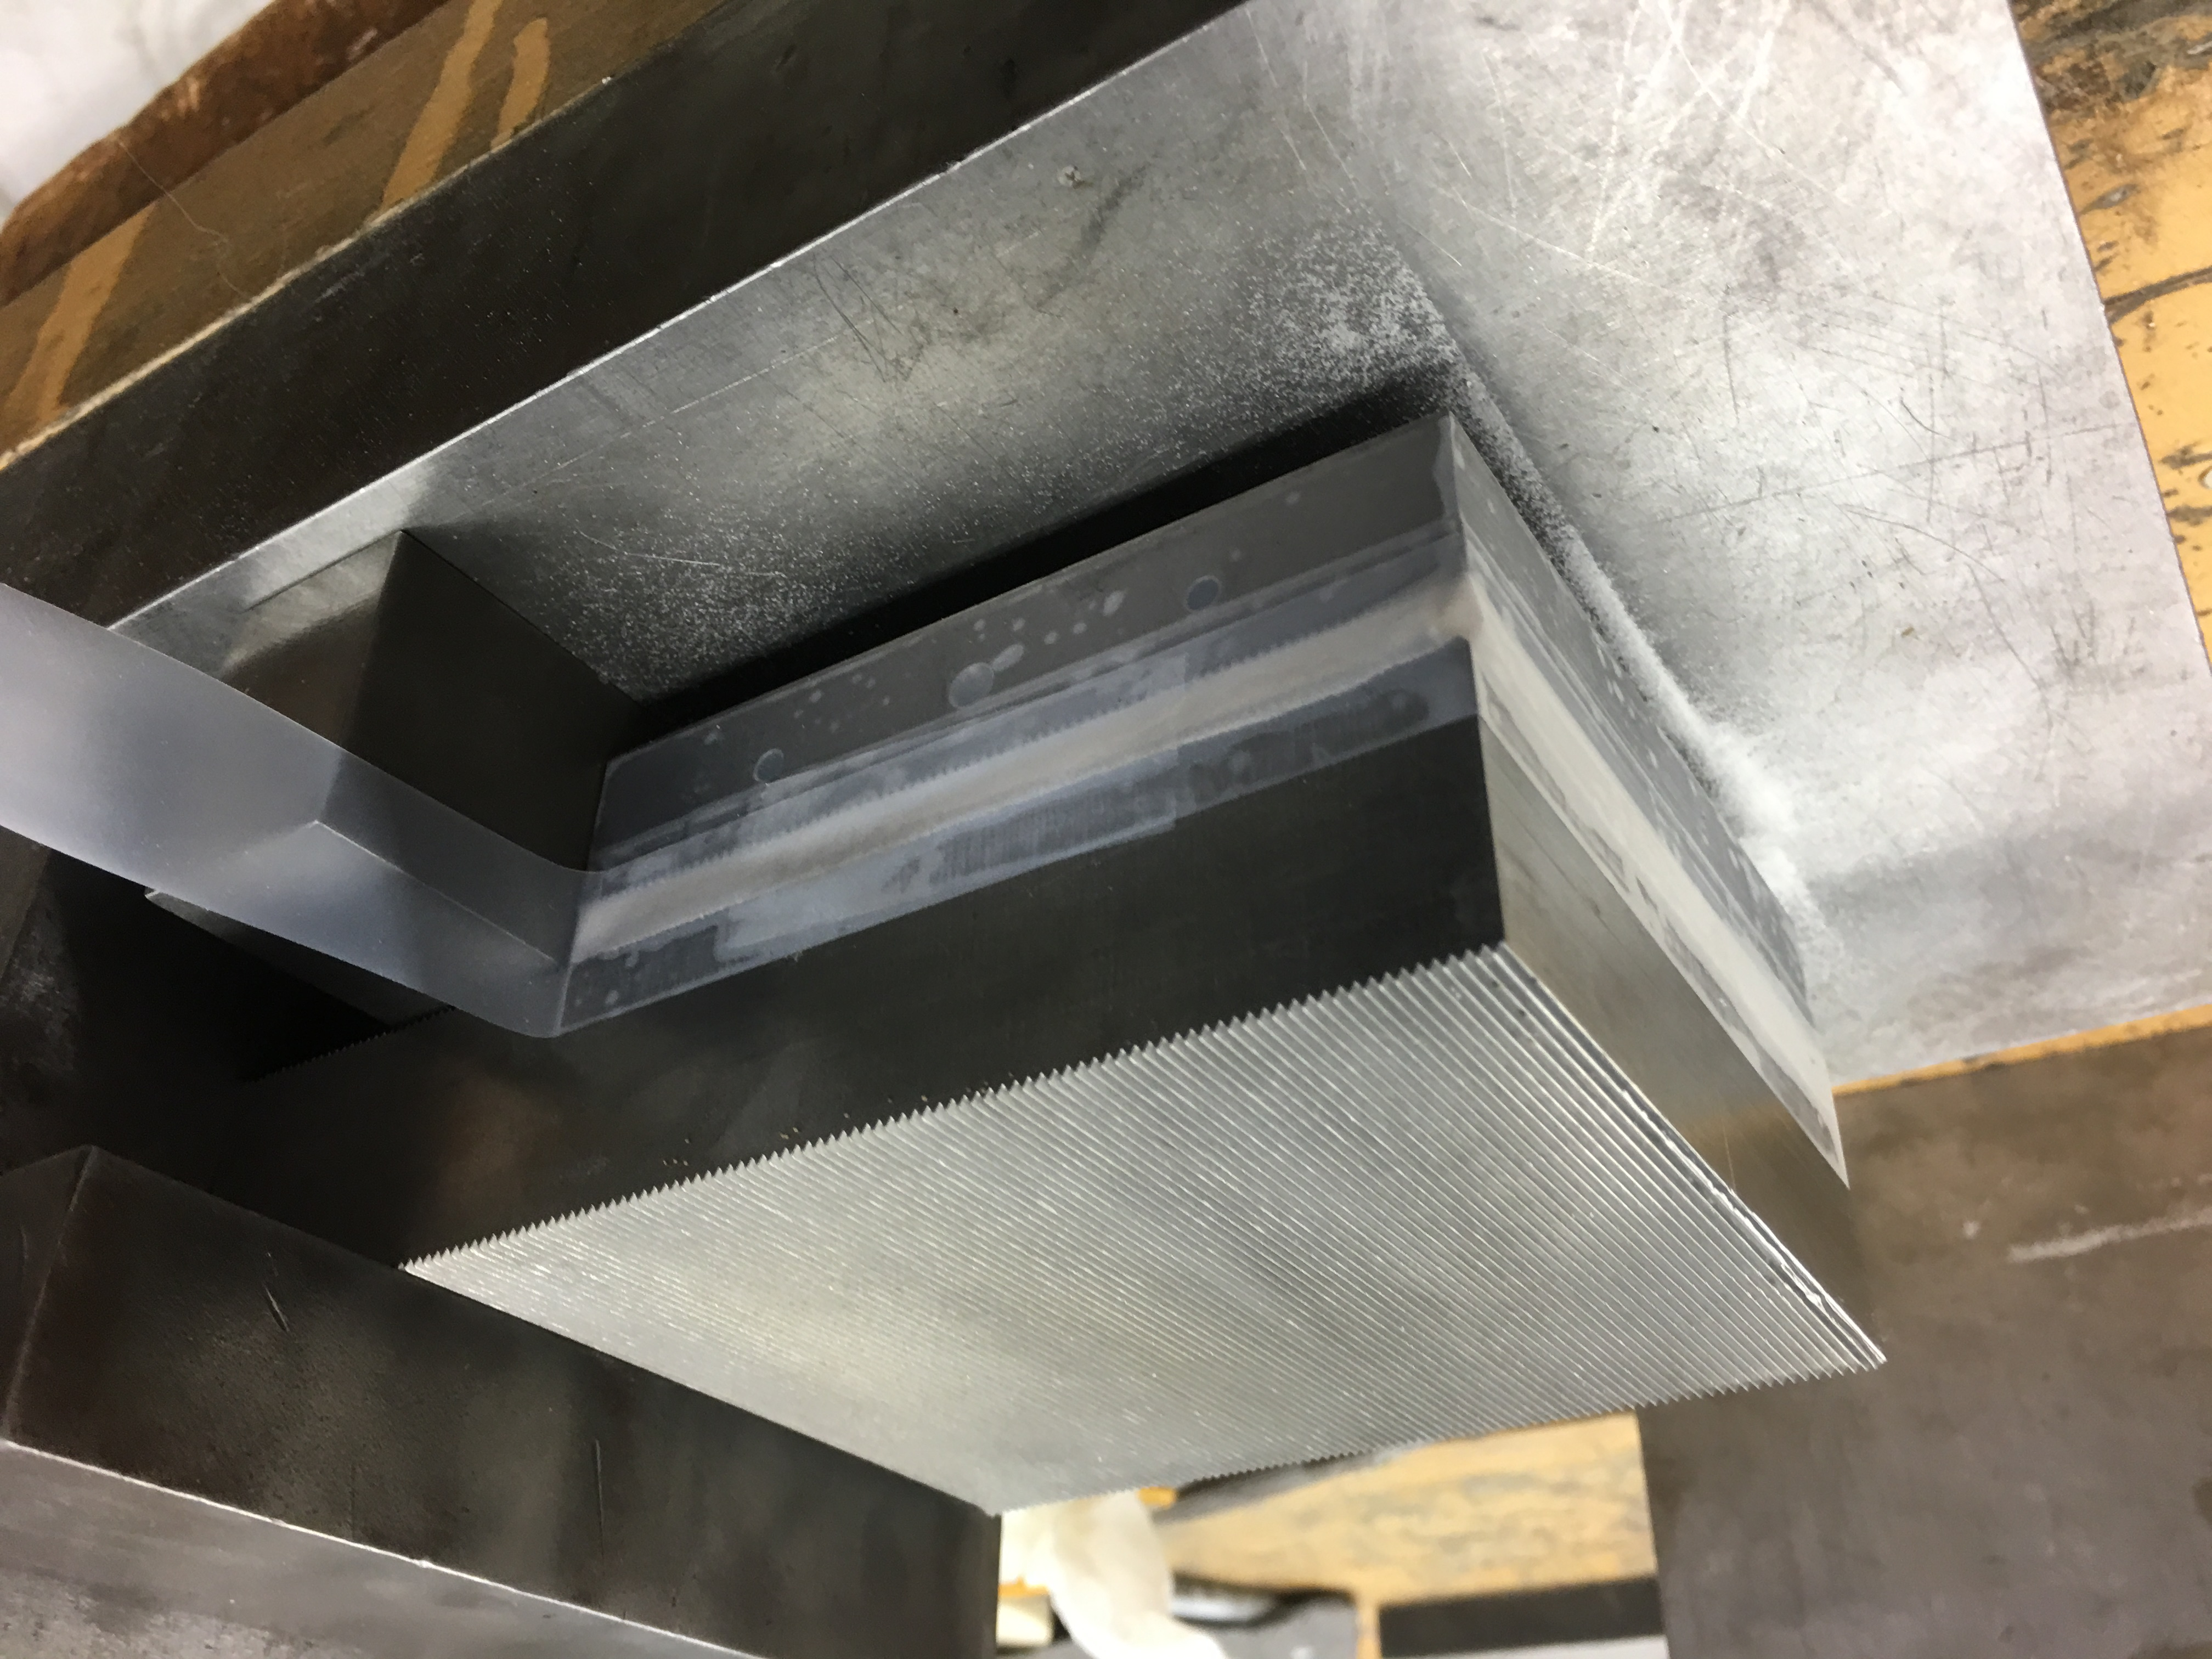
\includegraphics[width=0.7\textwidth]{appendix_sample_prep/dds_one_strip_tape.jpg}
   	\caption{Place one strip of tape around the bottom and sides of the sample.}
  	\label{Fig:dds_one_strip_tape}
\end{figure}
%% End Figure %%

\clearpage

%% Figure %%
\begin{figure}
	\centering
        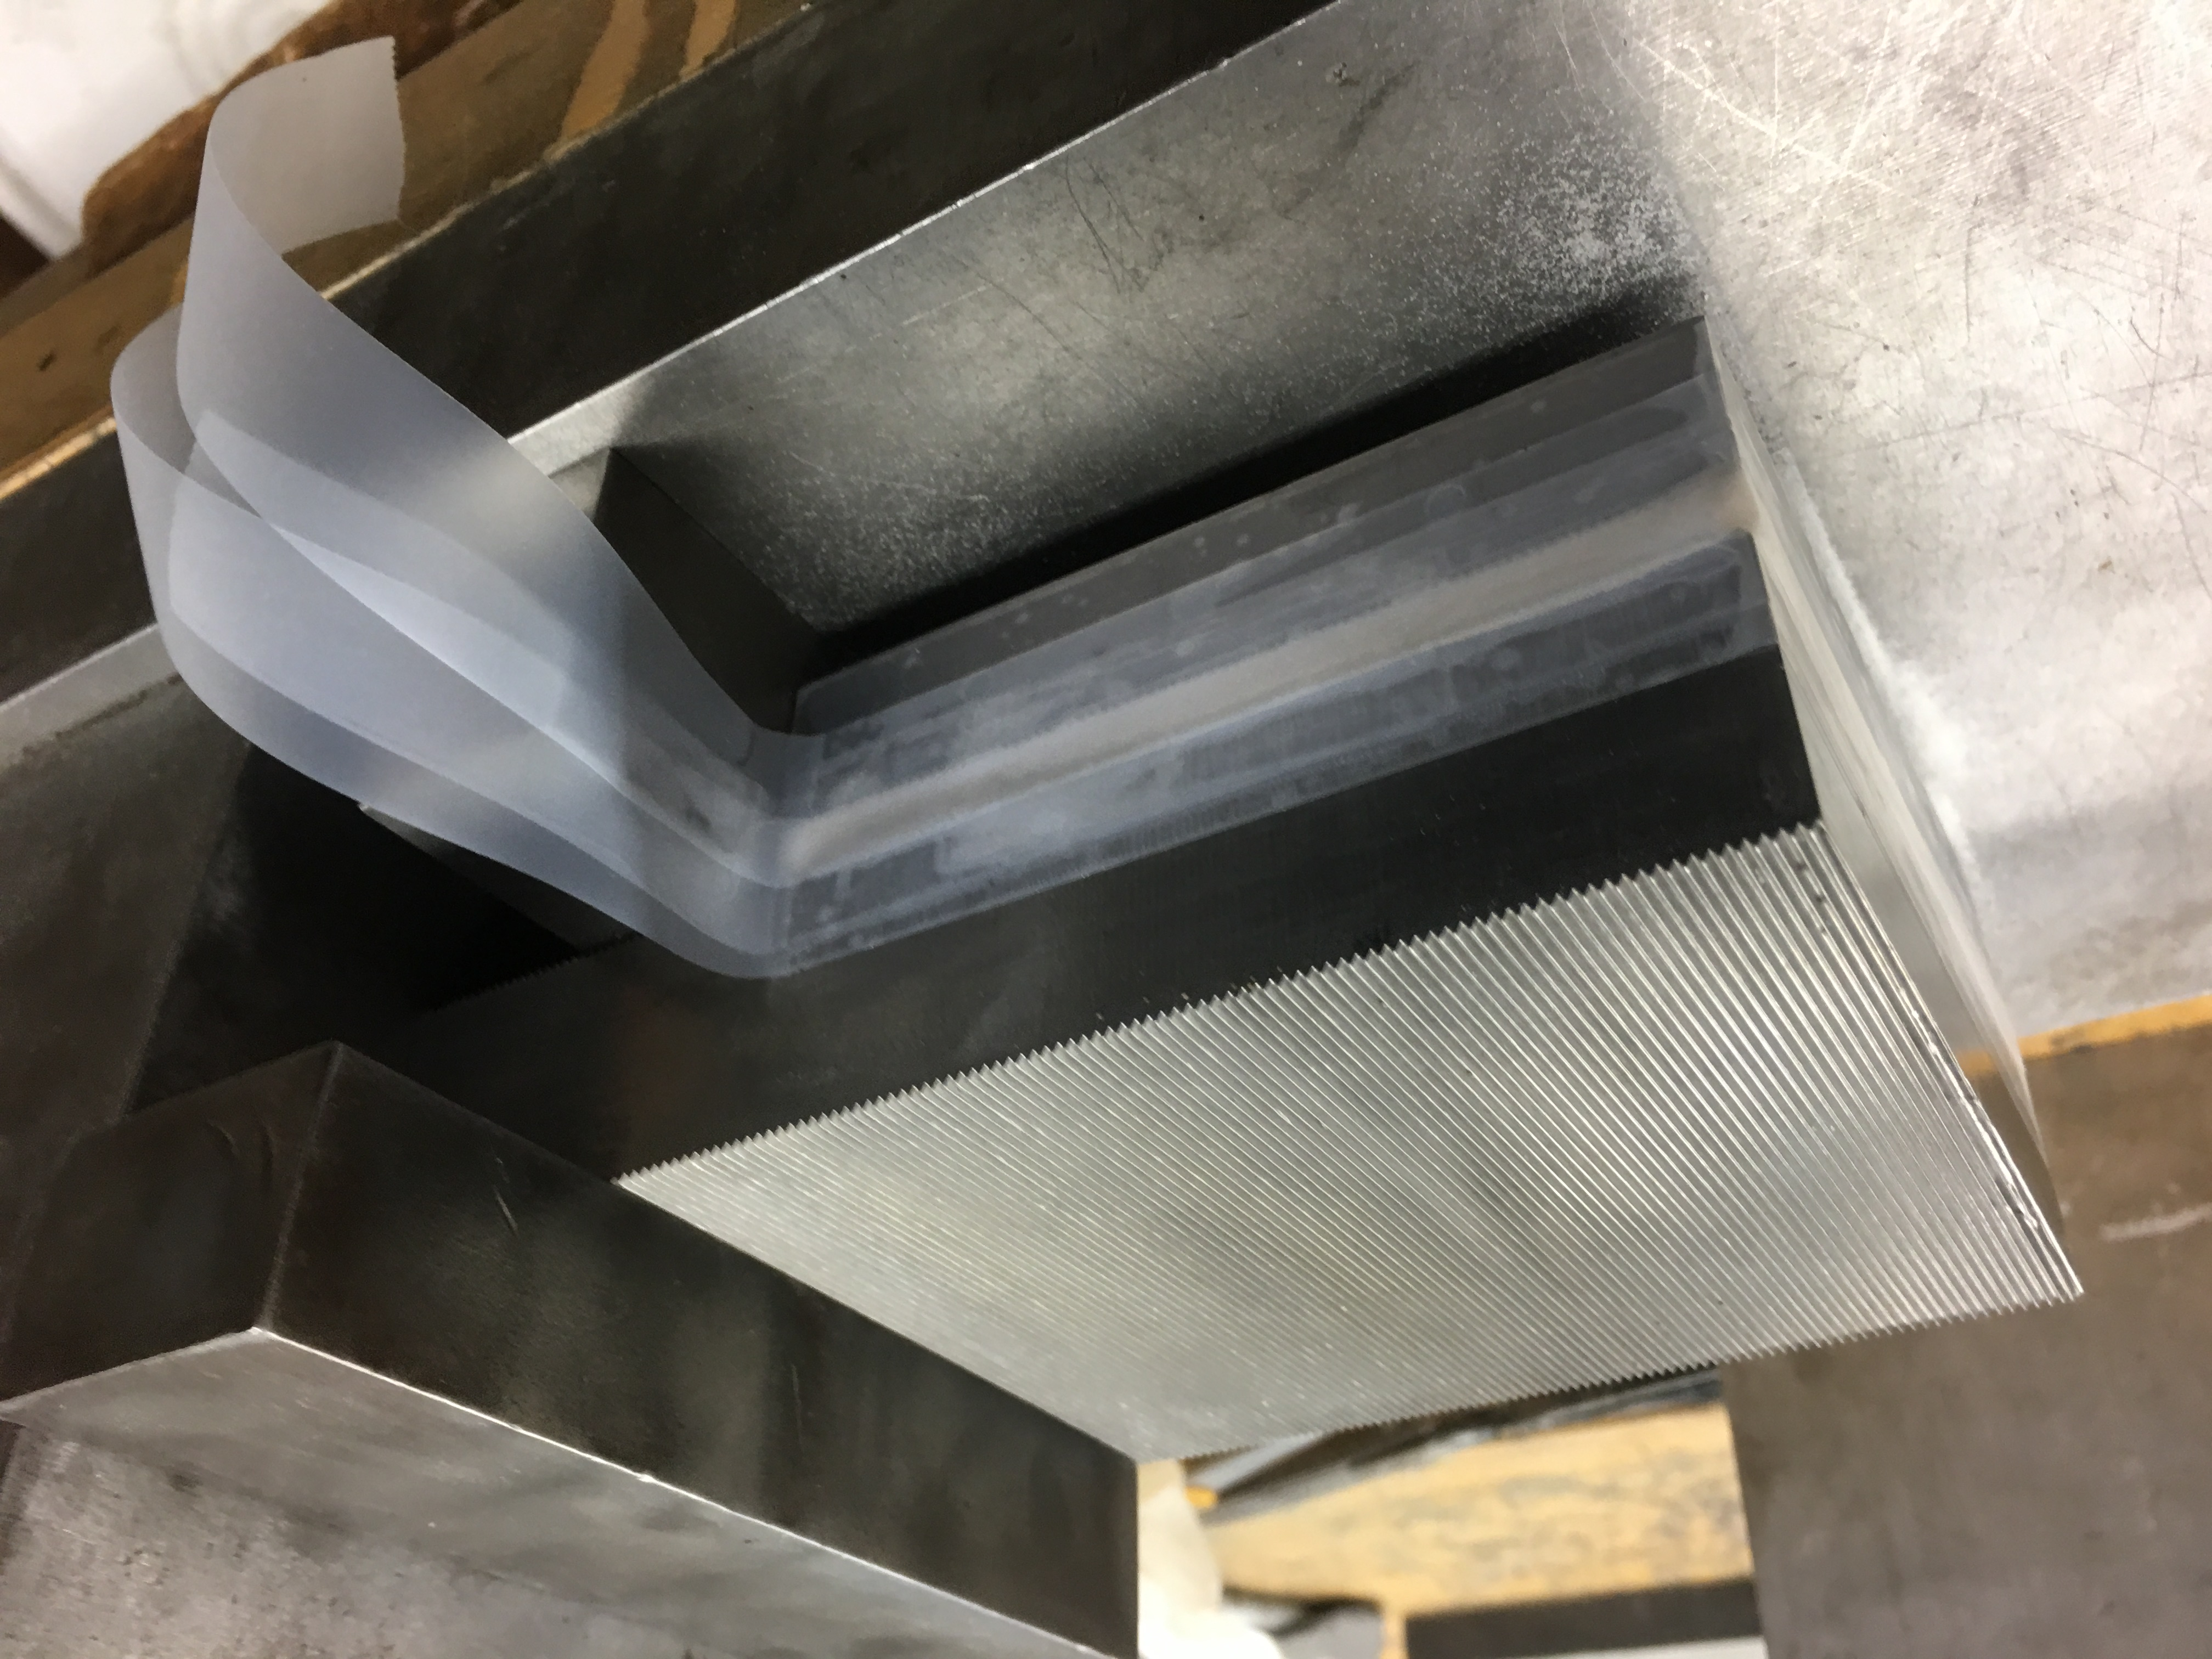
\includegraphics[width=0.7\textwidth]{appendix_sample_prep/dds_three_strip_tape.jpg}
   	\caption{Add two more strips of tape, each offset from the others to provide the best seal of the sample material.}
  	\label{Fig:dds_three_strip_tape}
\end{figure}
%% End Figure %%

%% Figure %%
\begin{figure}
	\centering
        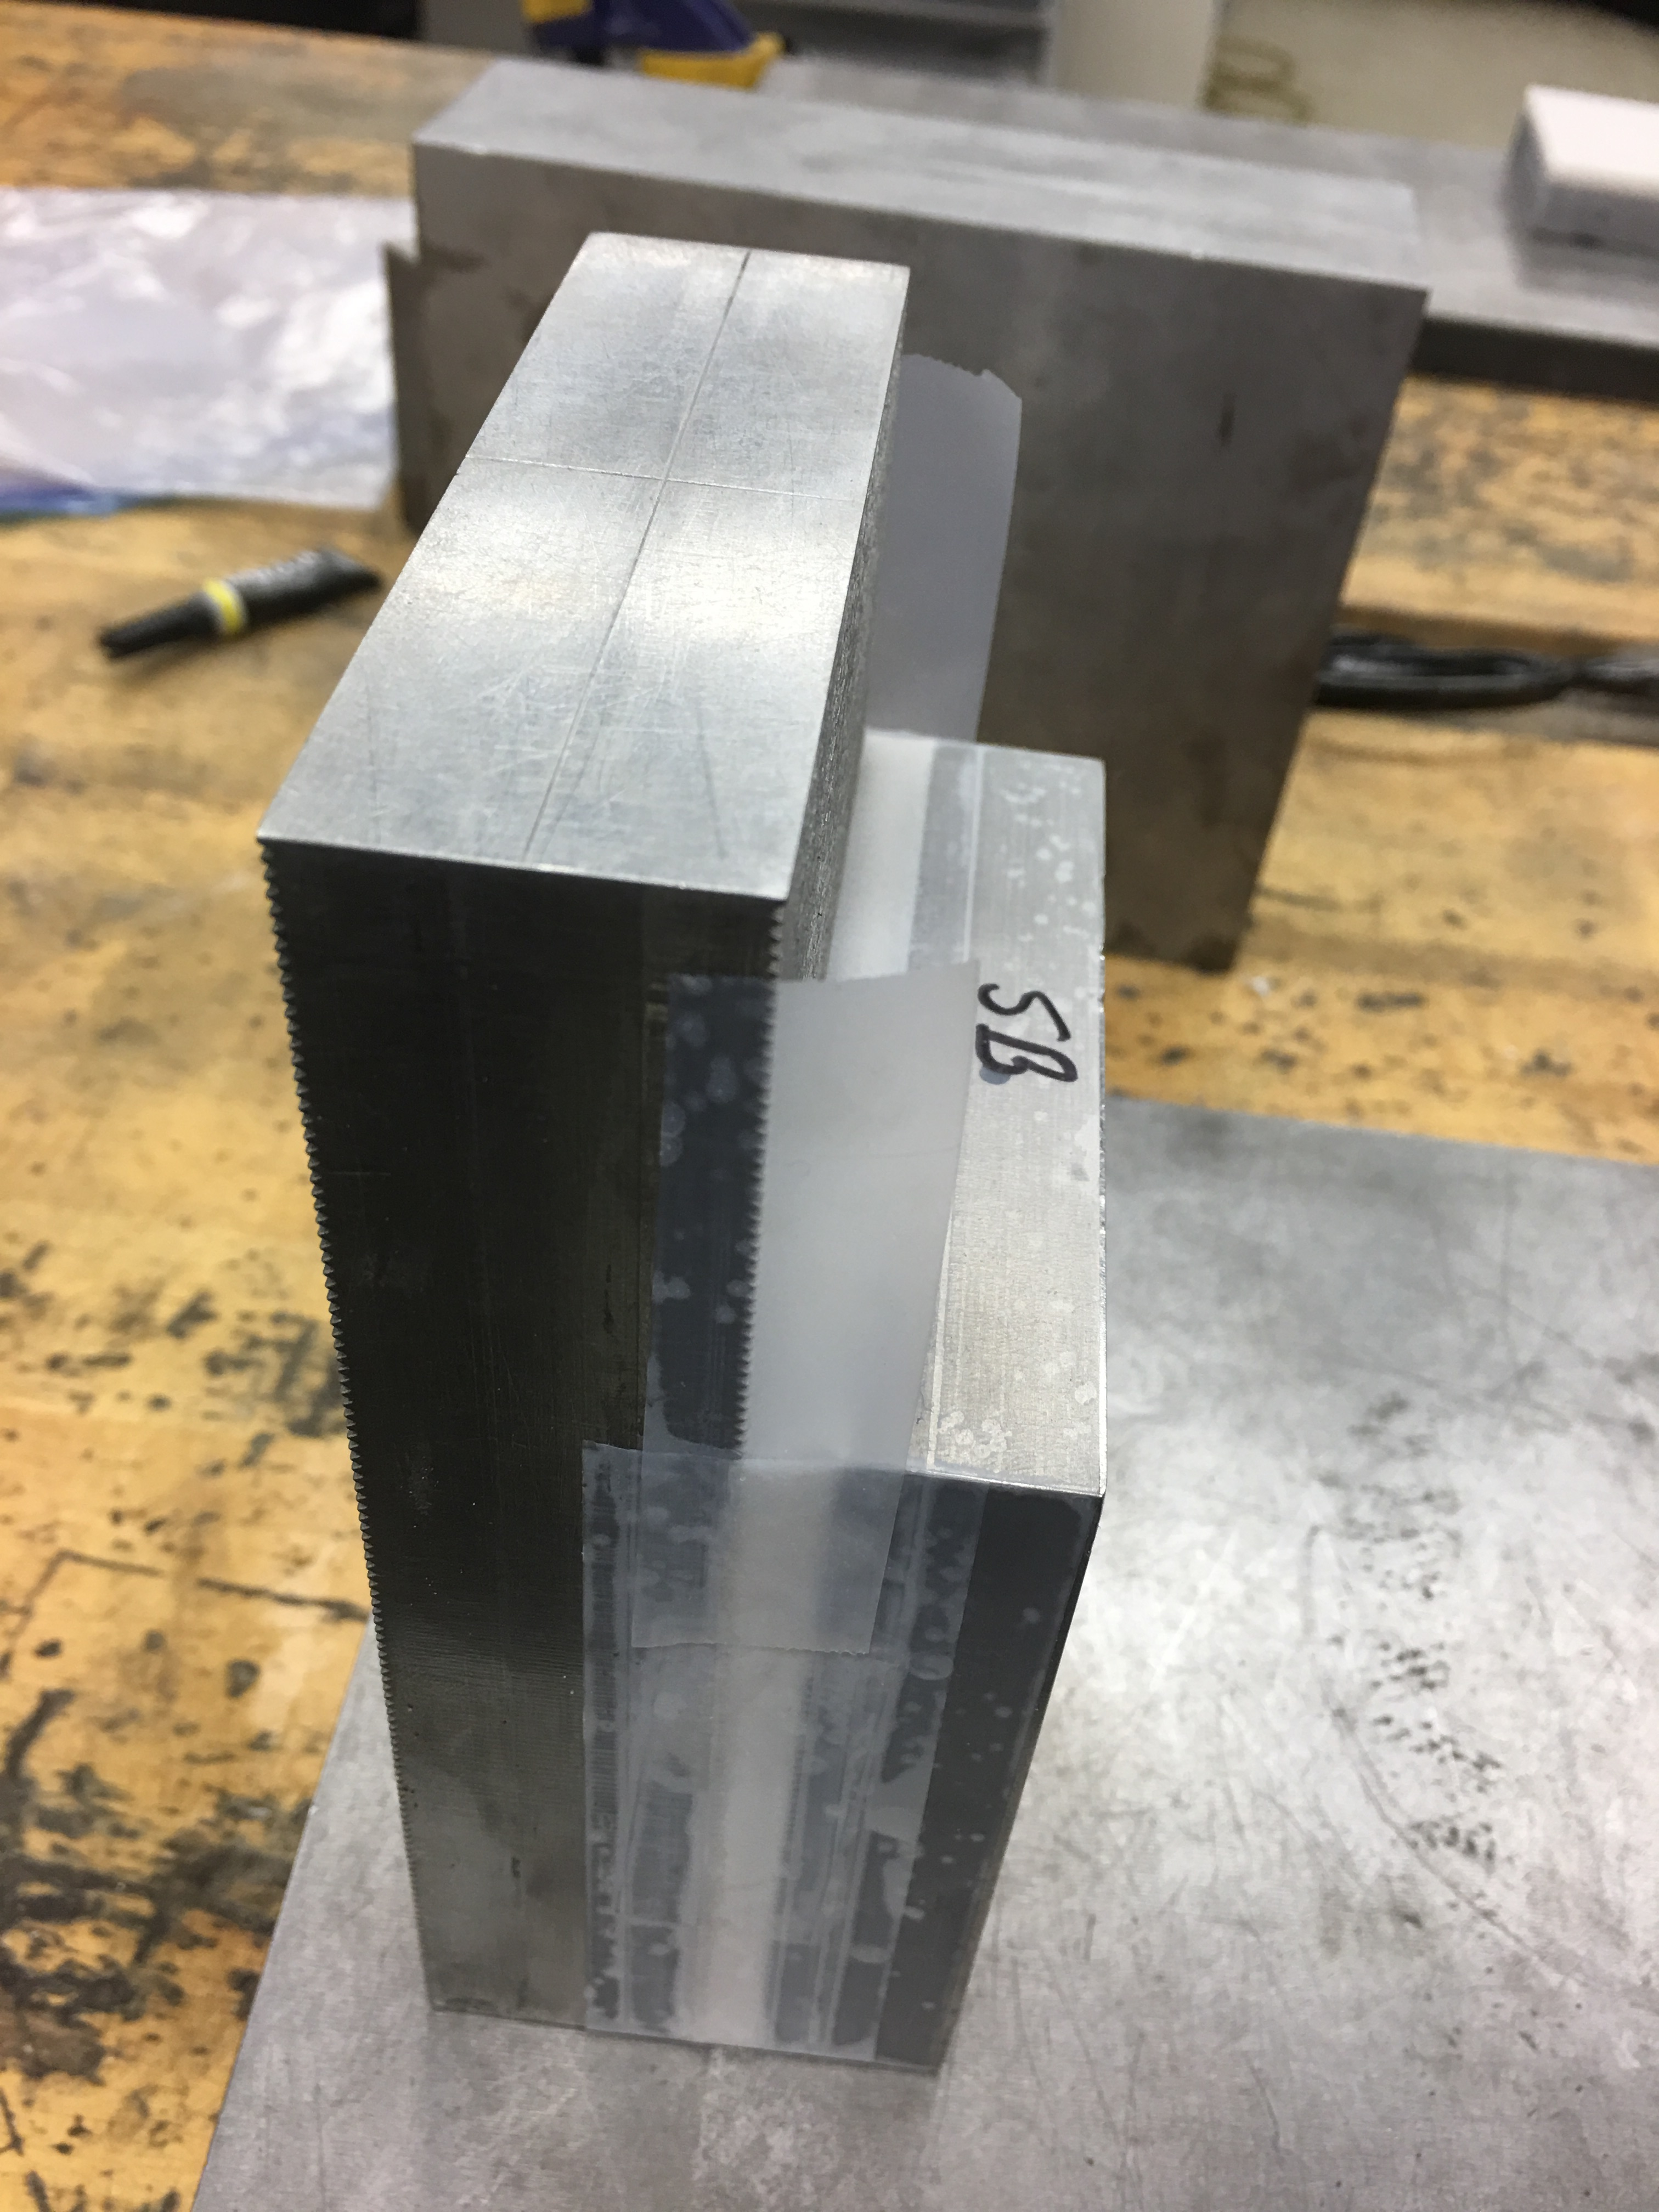
\includegraphics[width=0.7\textwidth]{appendix_sample_prep/dds_standup_one_block.jpg}
   	\caption{Stand the assembly up on the workbench.}
  	\label{Fig:dds_standup_one_block}
\end{figure}
%% End Figure %%

%% Figure %%
\begin{figure}
	\centering
        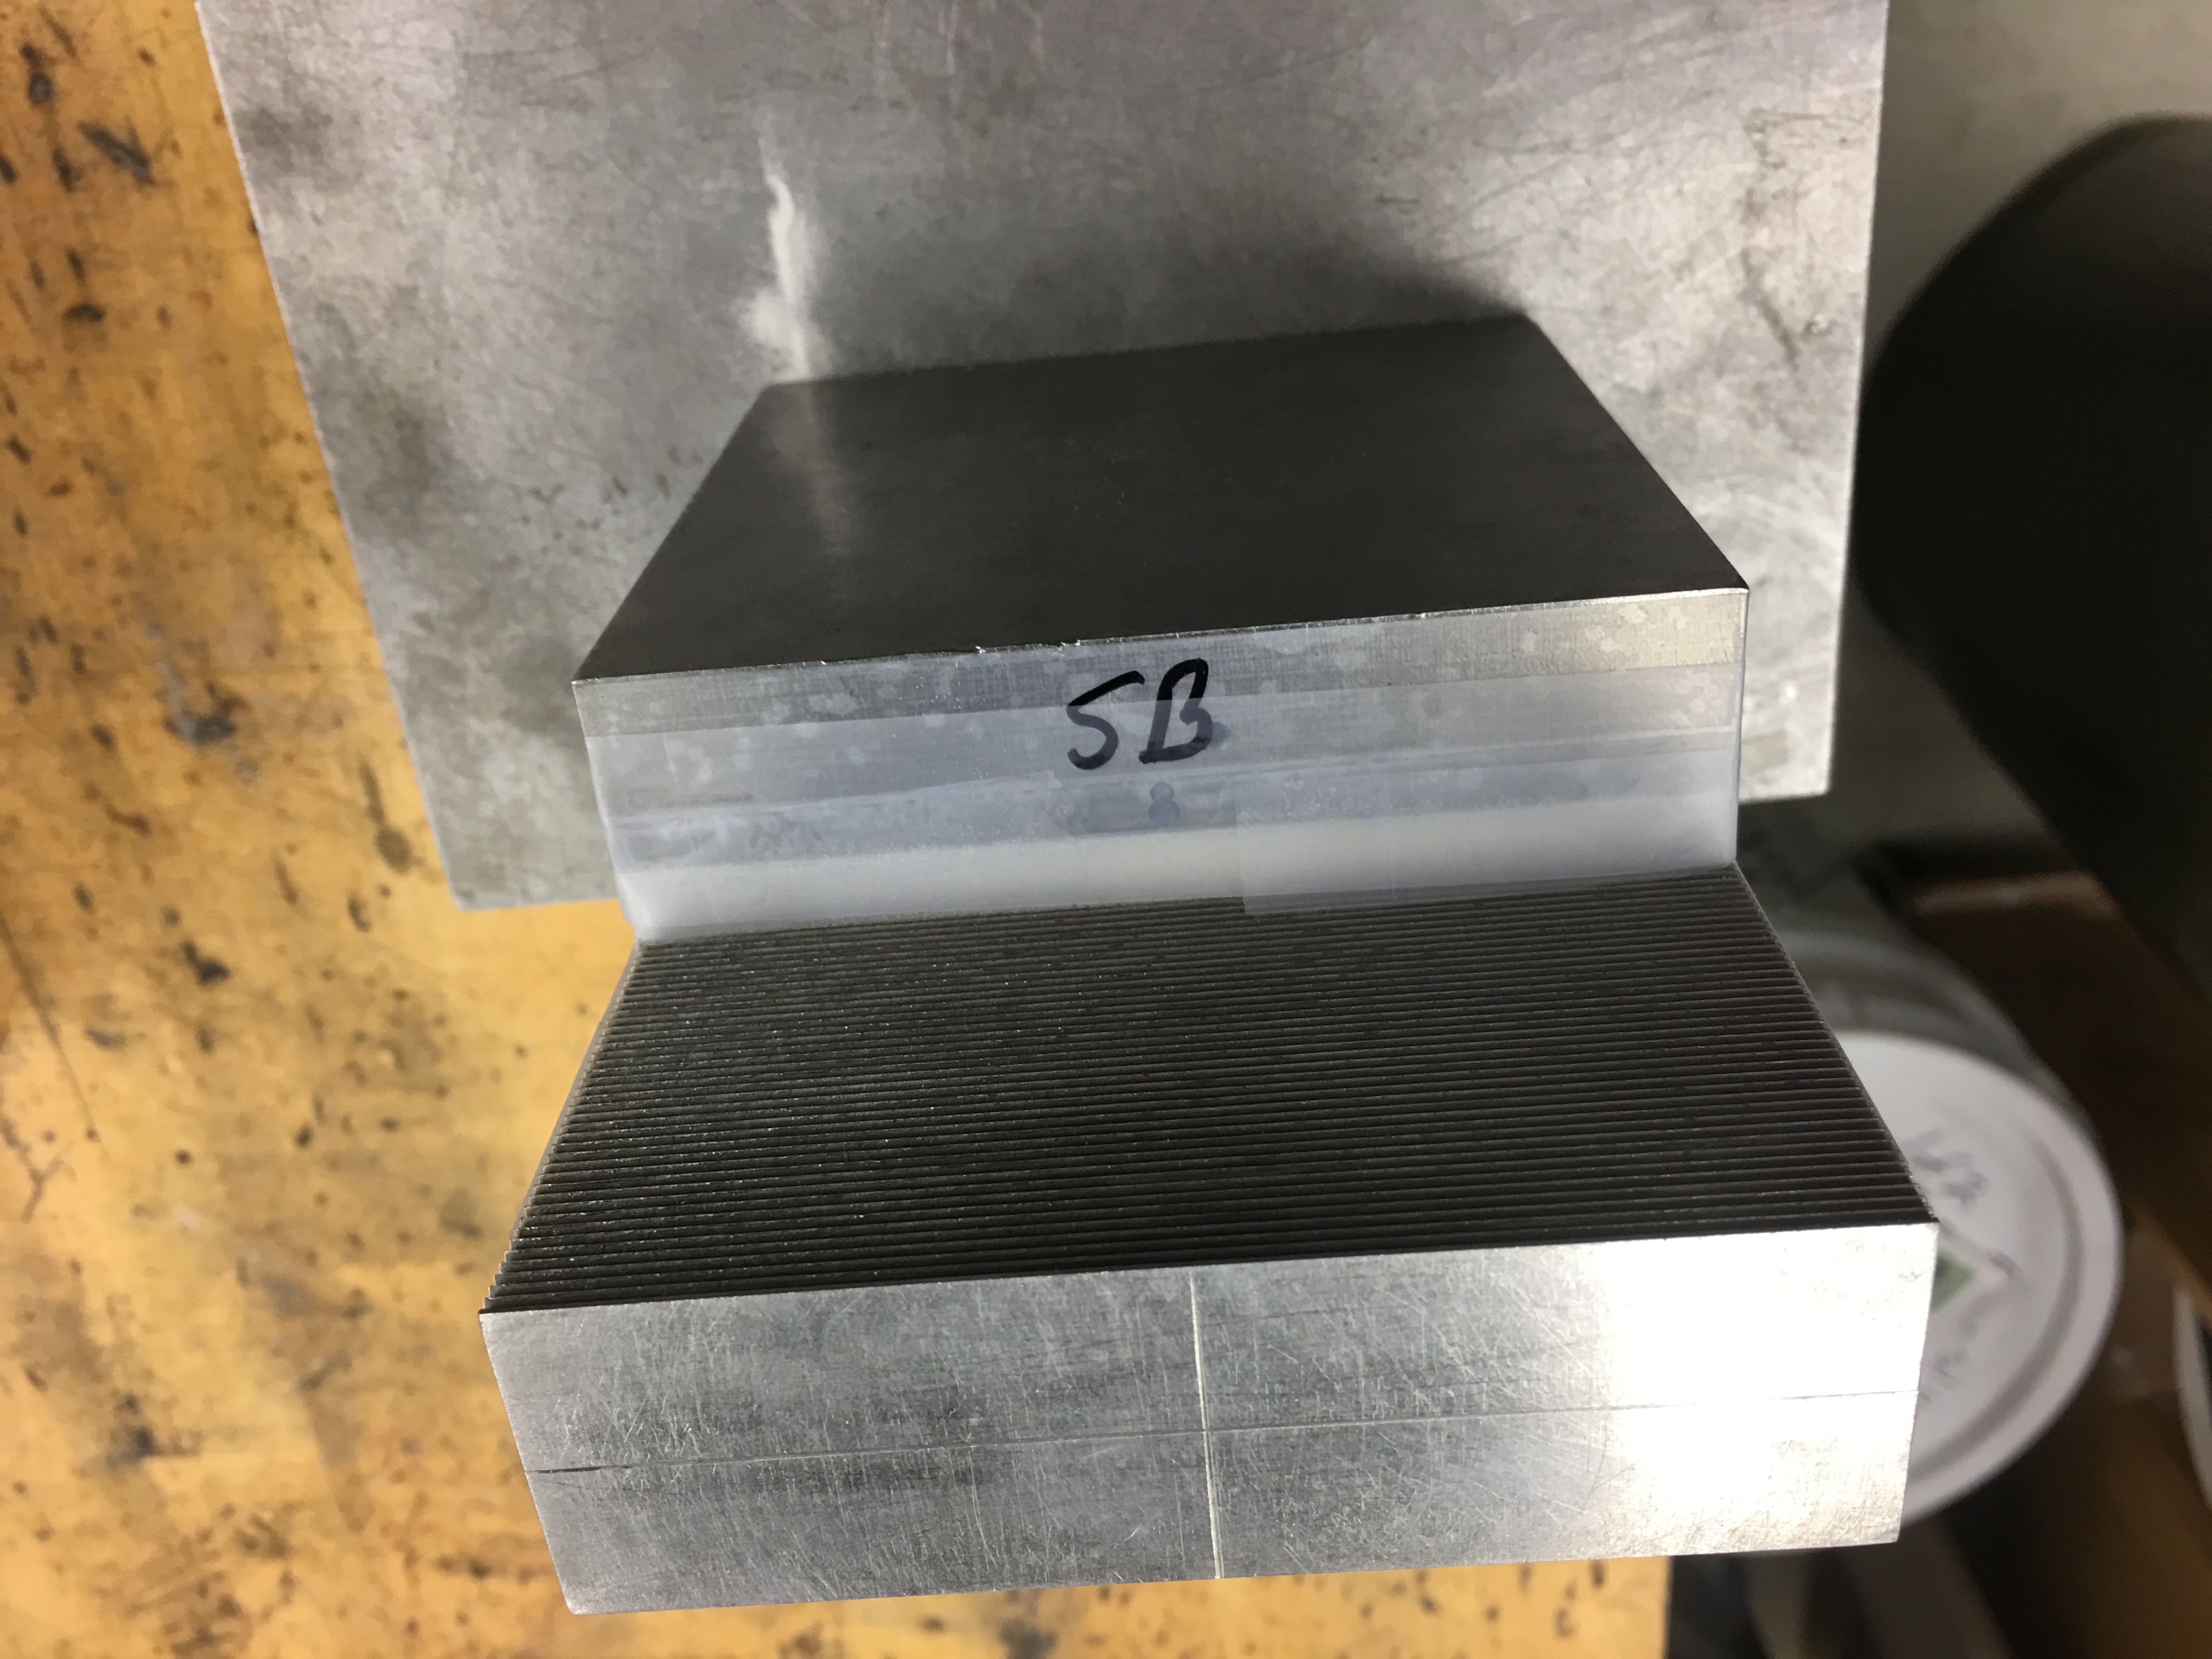
\includegraphics[width=0.7\textwidth]{appendix_sample_prep/dds_one_block_taped.jpg}
   	\caption{Tape the top of the assembly.}
  	\label{Fig:dds_one_block_taped}
\end{figure}
%% End Figure %%

%% Figure %%
\begin{figure}
	\centering
        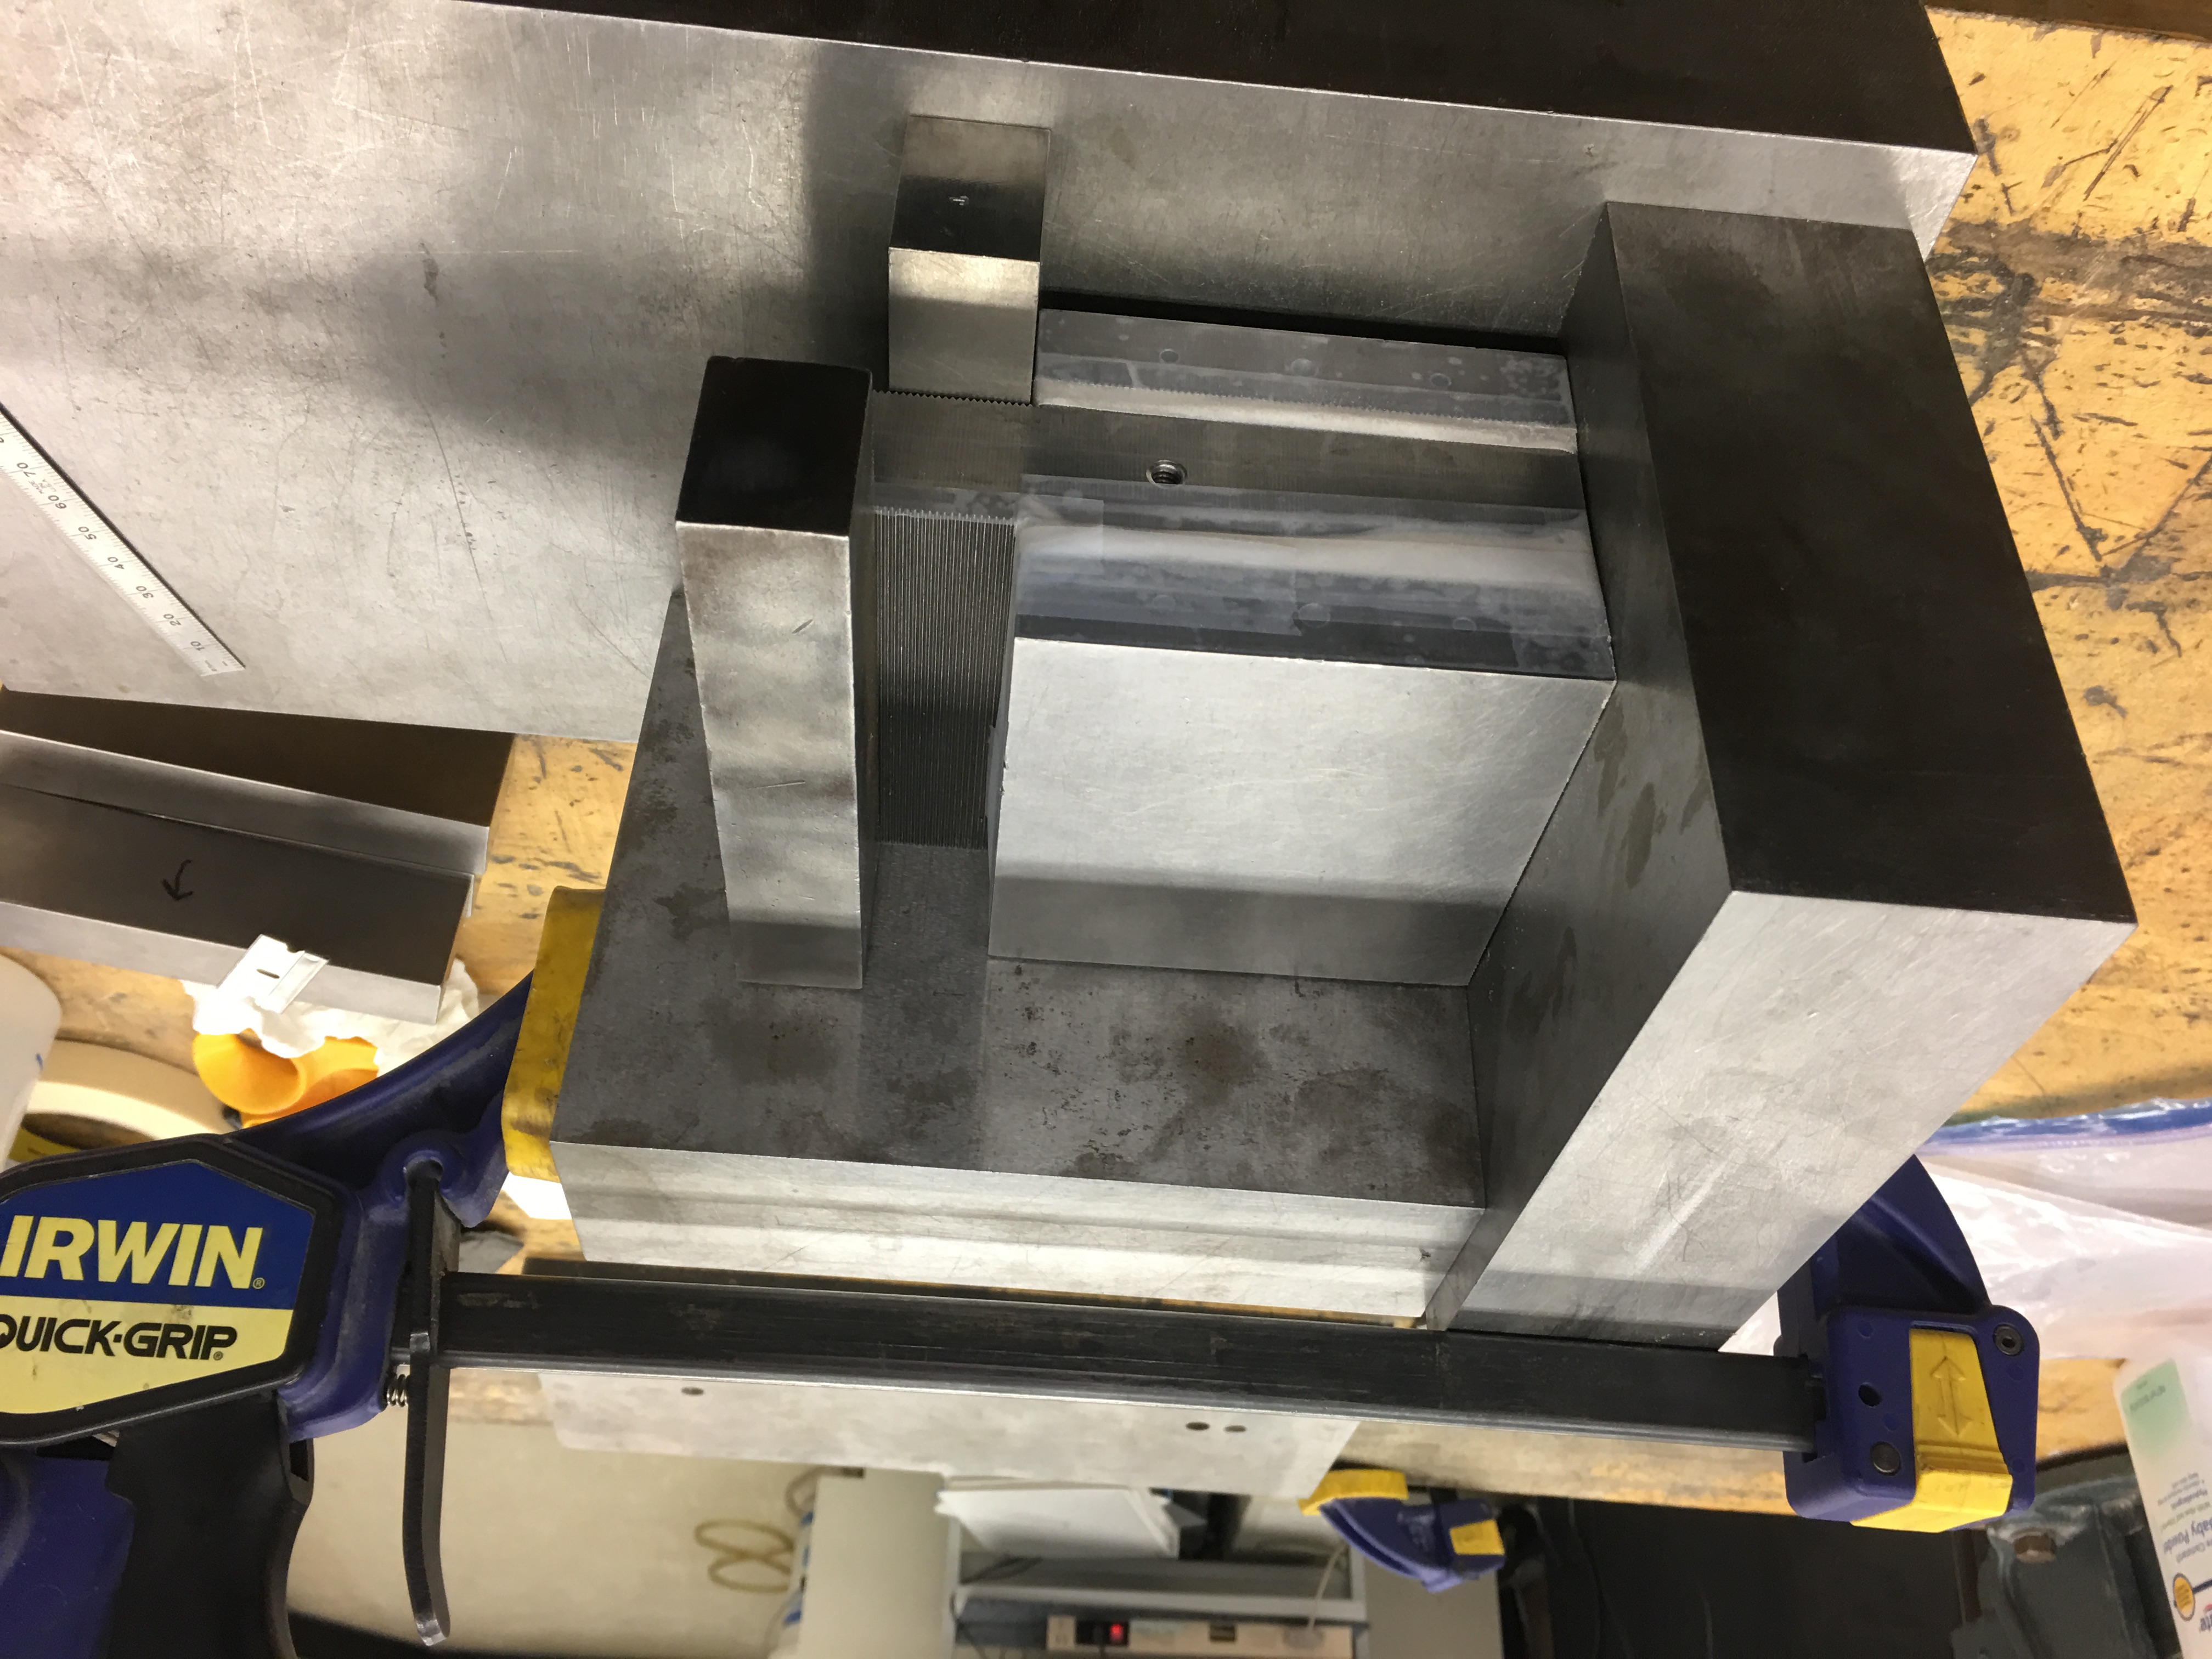
\includegraphics[width=0.7\textwidth]{appendix_sample_prep/dds_two_block_jig.jpg}
   	\caption{Follow the same procedure to add the second side block to the assembly.}
  	\label{Fig:dds_two_block_jig}
\end{figure}
%% End Figure %%

\clearpage

%% Figure %%
\begin{figure}
	\centering
        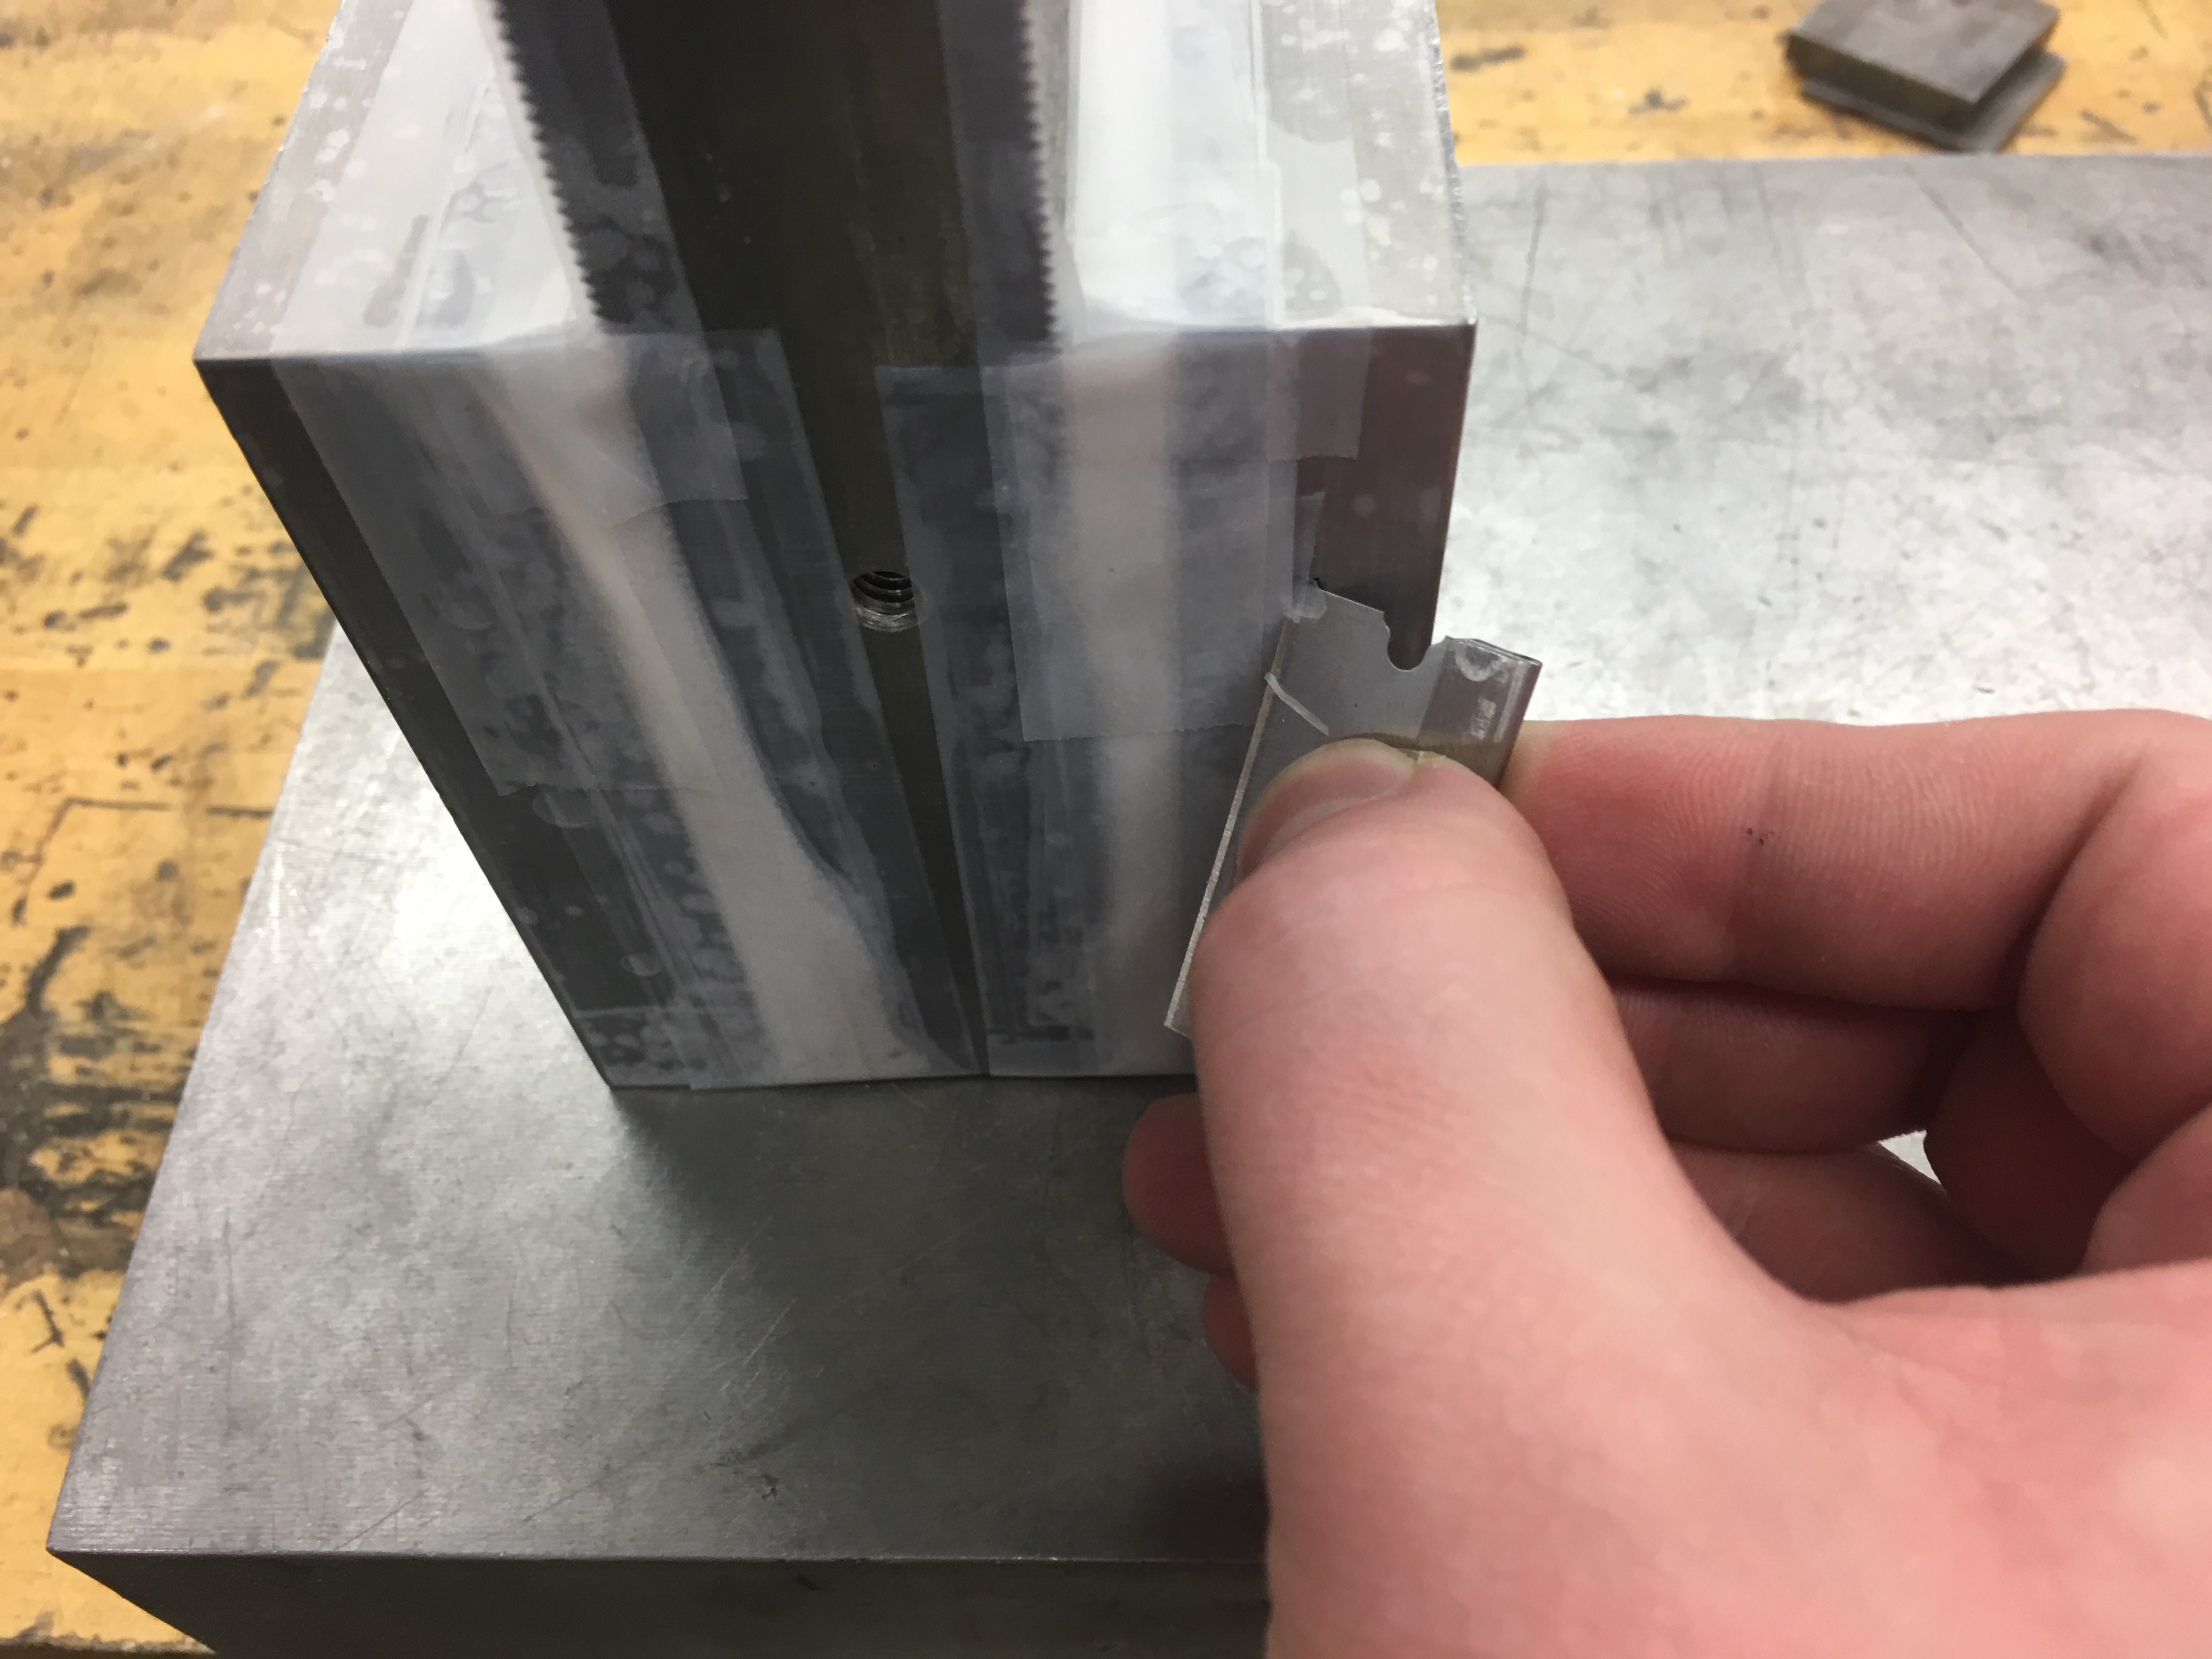
\includegraphics[width=0.7\textwidth]{appendix_sample_prep/dds_trim_holes.jpg}
   	\caption{Using a razor blade, carefully trim out the holes for mounting side shields on each side block.}
  	\label{Fig:dds_trim_holes}
\end{figure}
%% End Figure %%

%% Figure %%
\begin{figure}
	\centering
        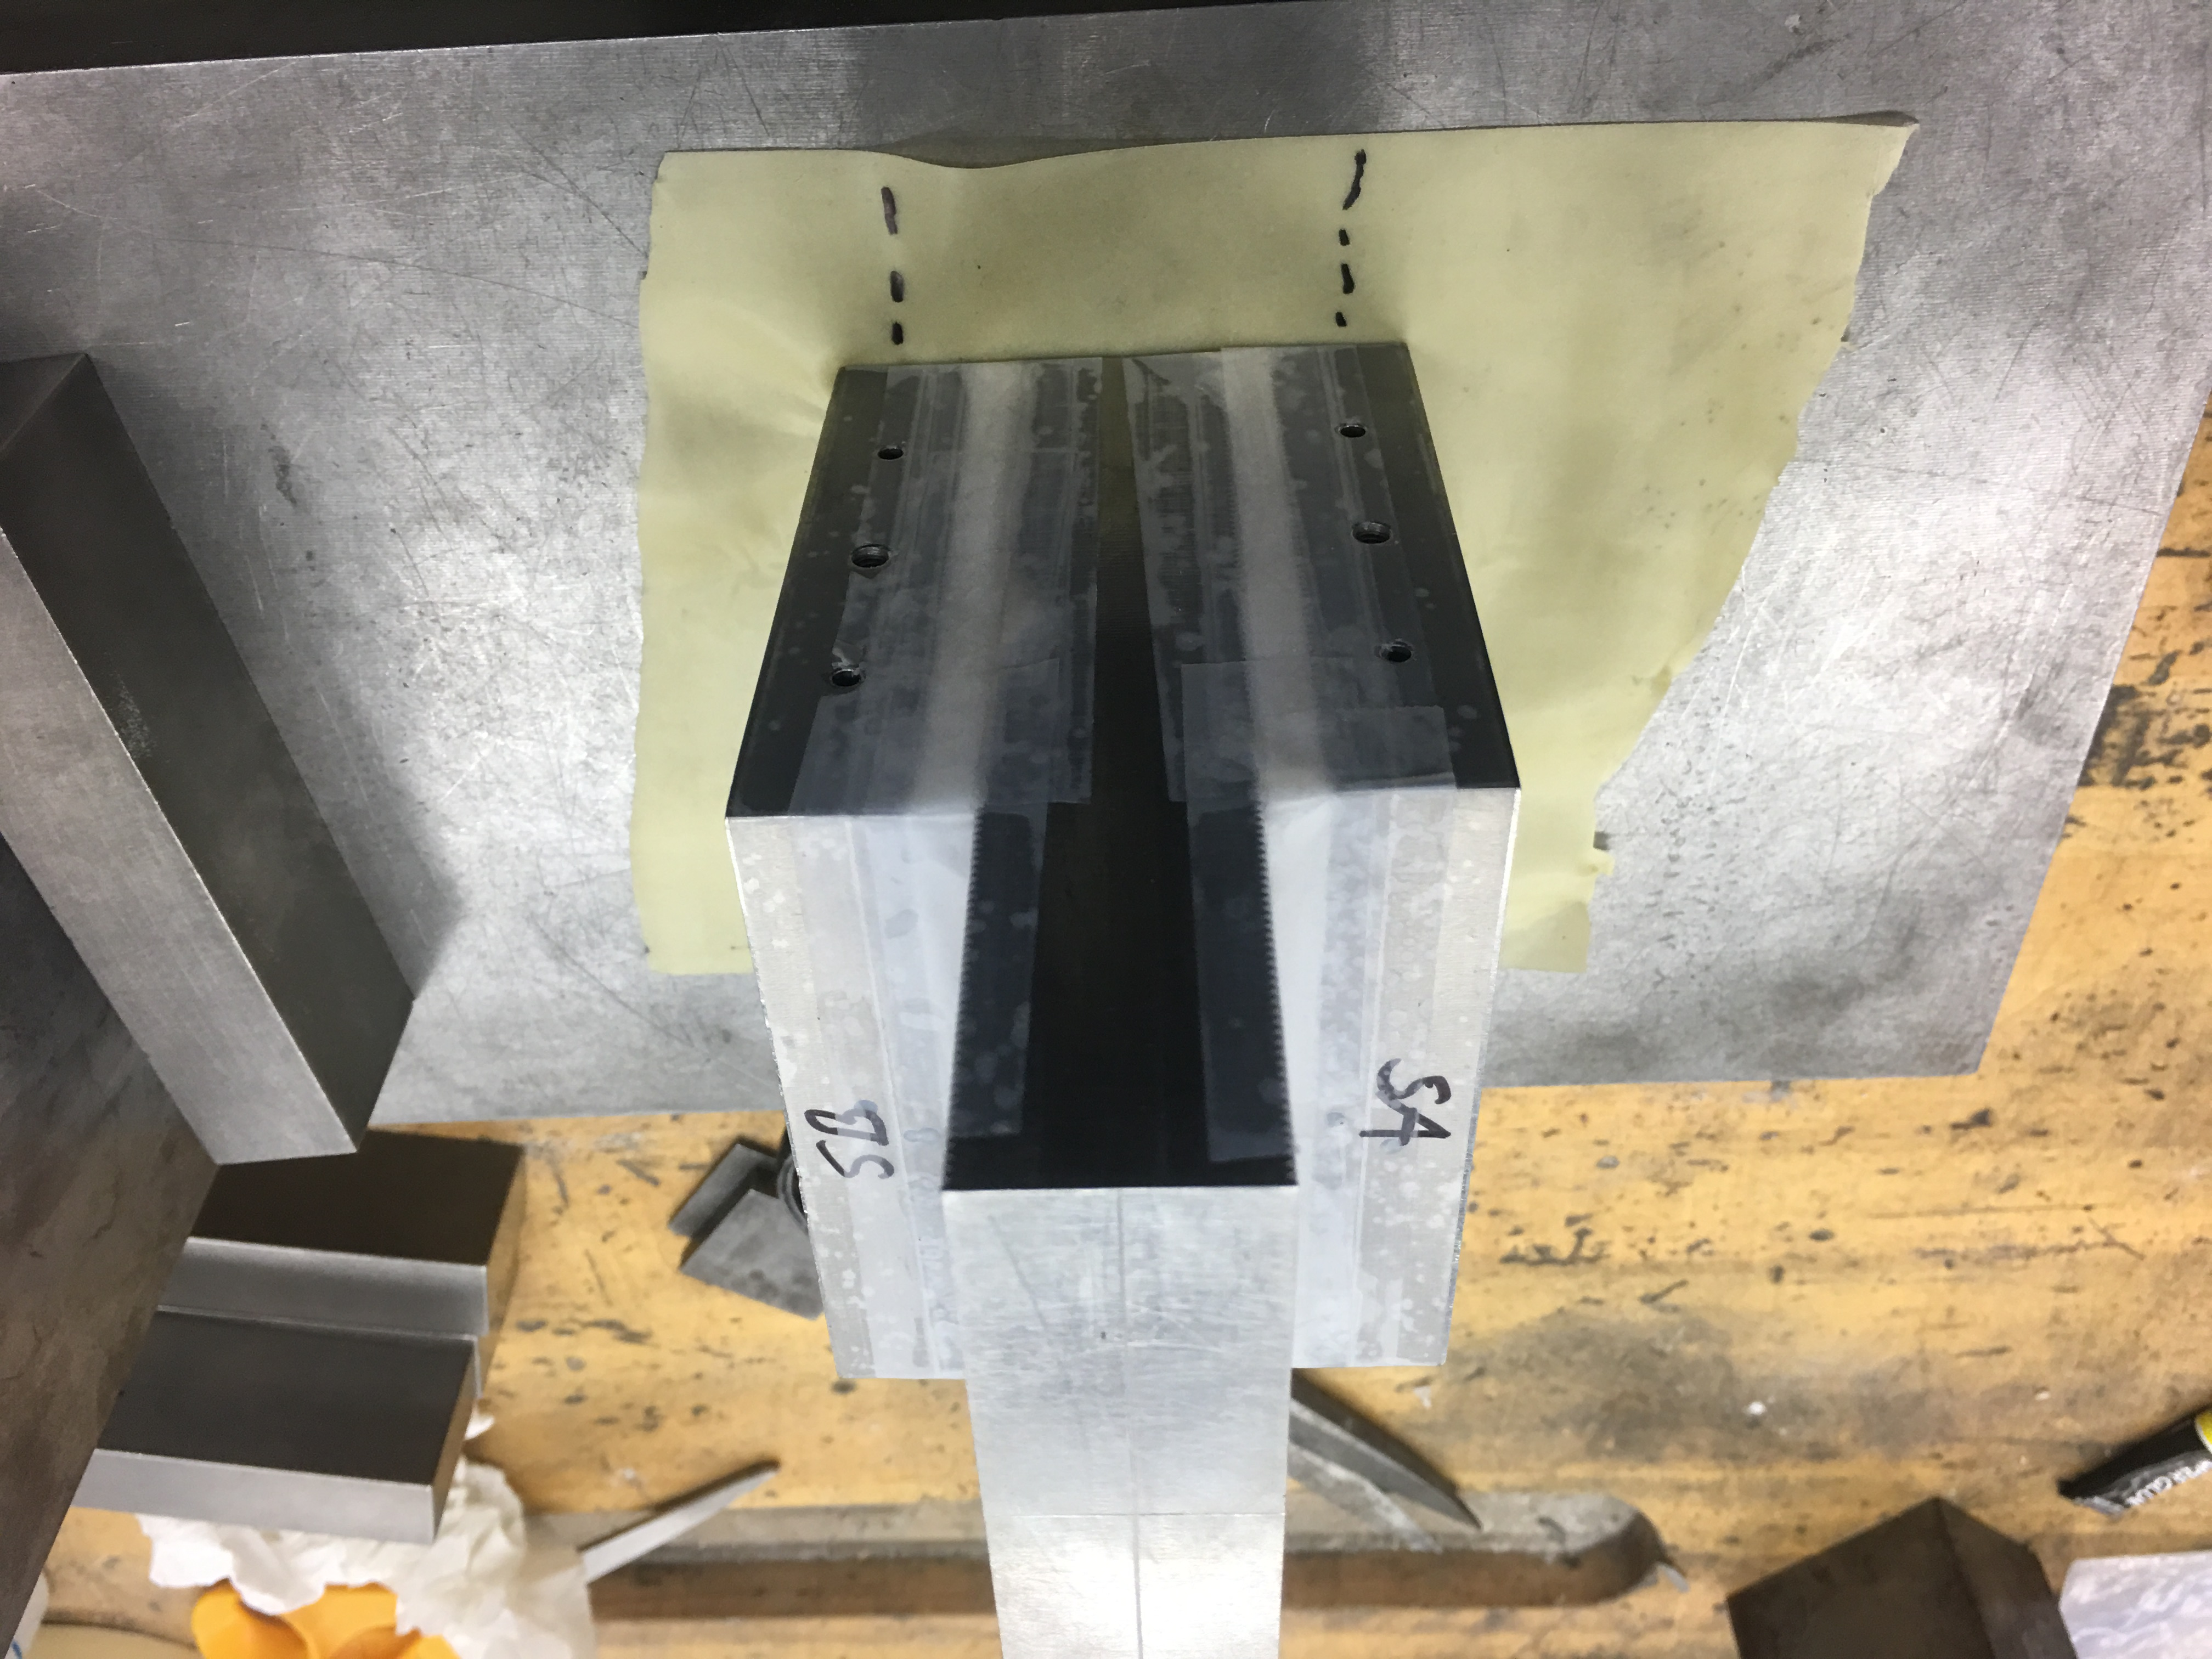
\includegraphics[width=0.7\textwidth]{appendix_sample_prep/dds_mark_rubber.jpg}
   	\caption{Mark the rubber skirt width and trim it to size.}
  	\label{Fig:dds_mark_rubber}
\end{figure}
%% End Figure %%

%% Figure %%
\begin{figure}
	\centering
        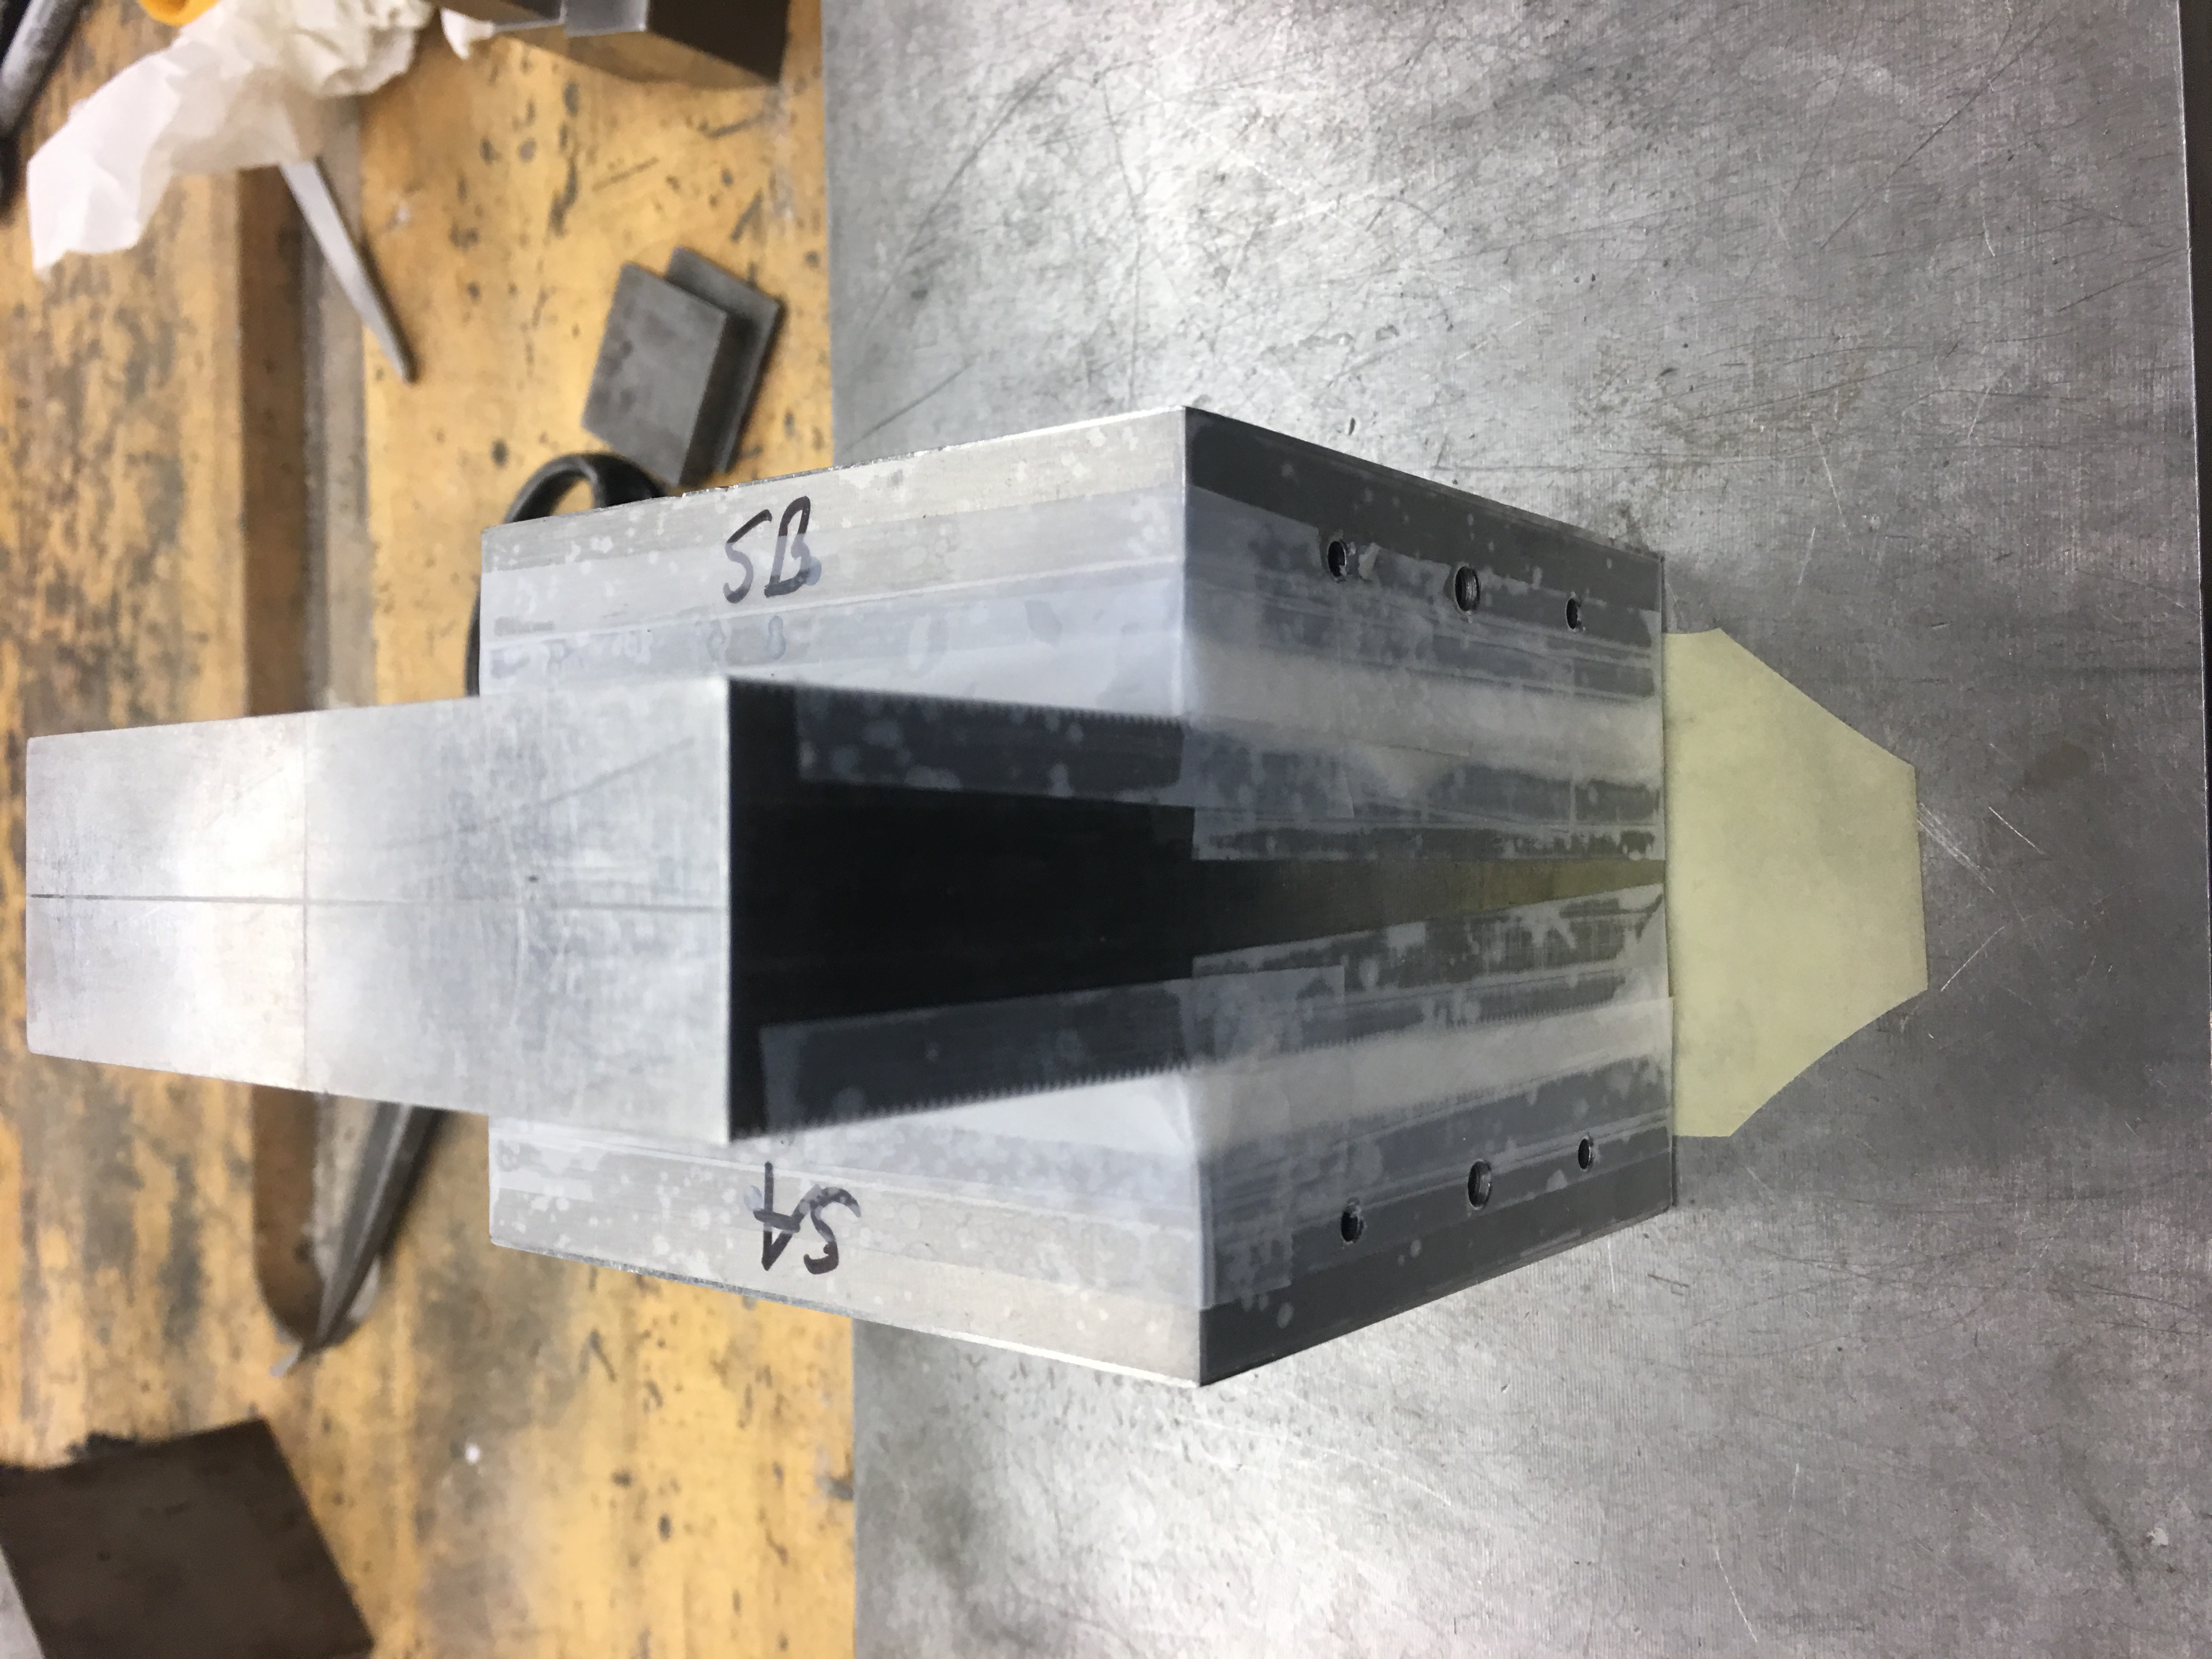
\includegraphics[width=0.7\textwidth]{appendix_sample_prep/dds_trimmed_rubber.jpg}
   	\caption{Position the trimmed rubber skirt beneath the sample and make sure that no side shield mounting points will be covered.}
  	\label{Fig:dds_trimmed_rubber}
\end{figure}
%% End Figure %%

%% Figure %%
\begin{figure}
	\centering
        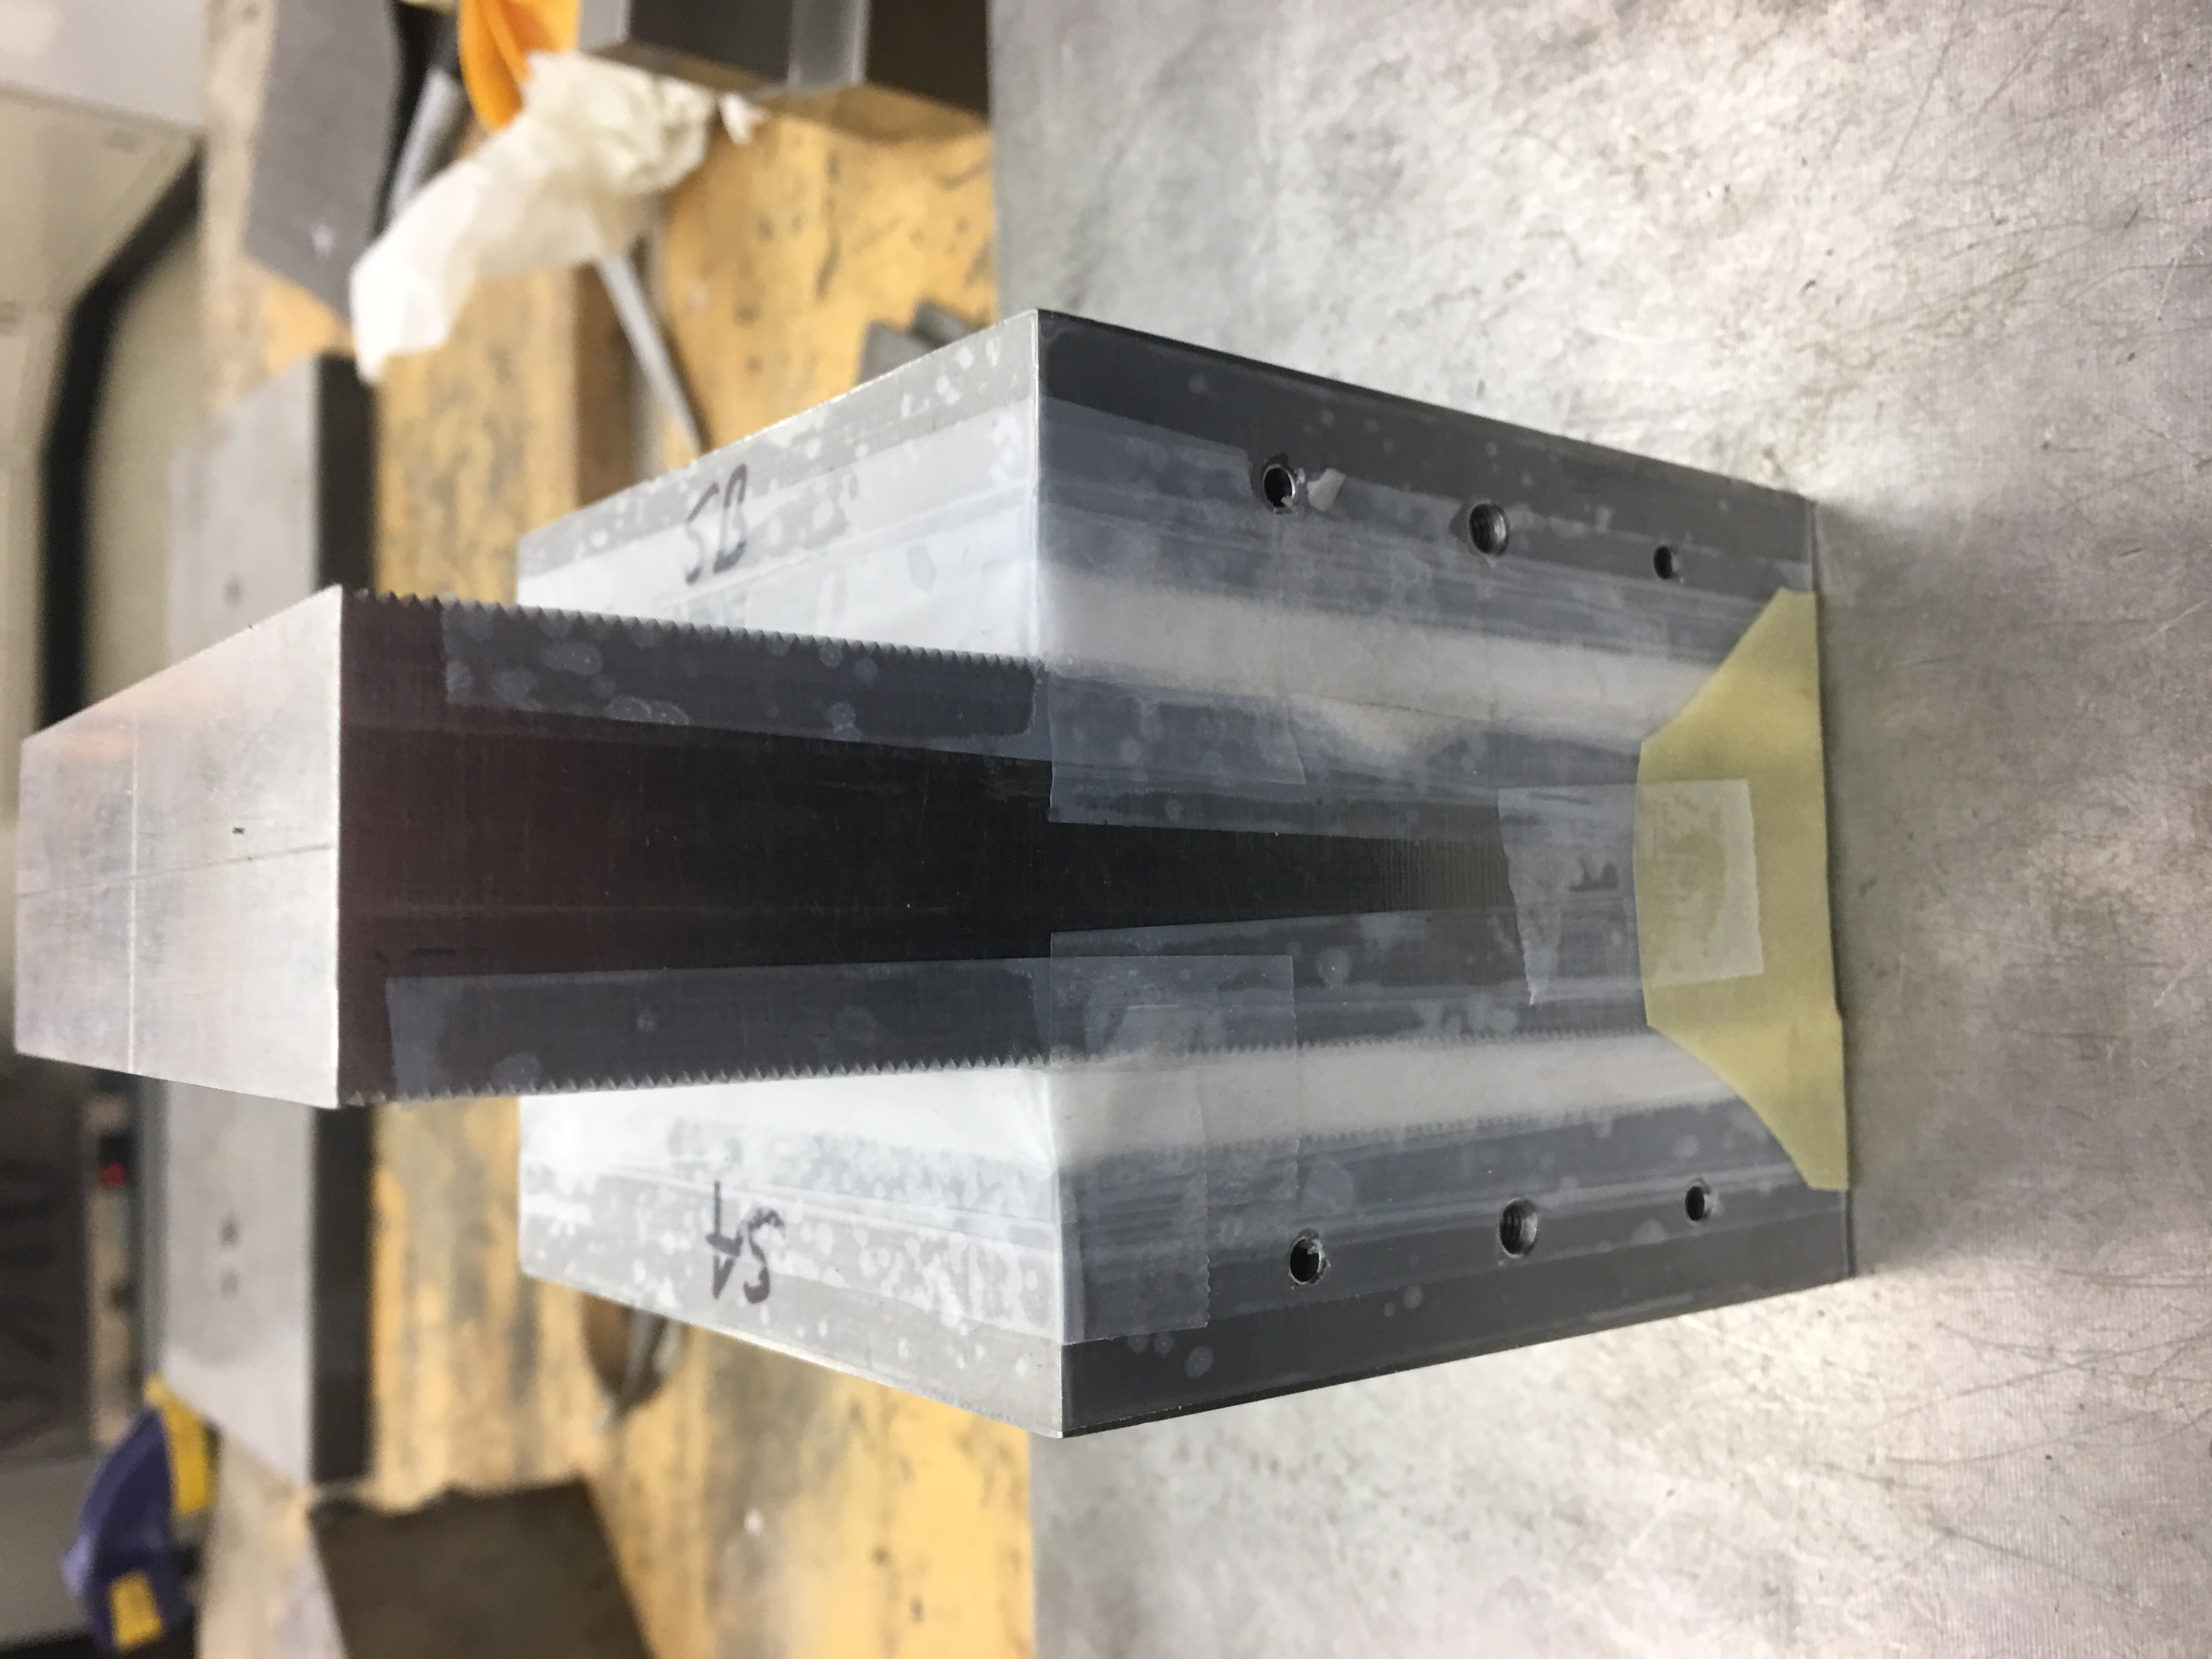
\includegraphics[width=0.7\textwidth]{appendix_sample_prep/dds_taped_rubber.jpg}
   	\caption{Temporarily secure the rubber skirt with tape.}
  	\label{Fig:dds_taped_rubber}
\end{figure}
%% End Figure %%

\clearpage

%% Figure %%
\begin{figure}
	\centering
        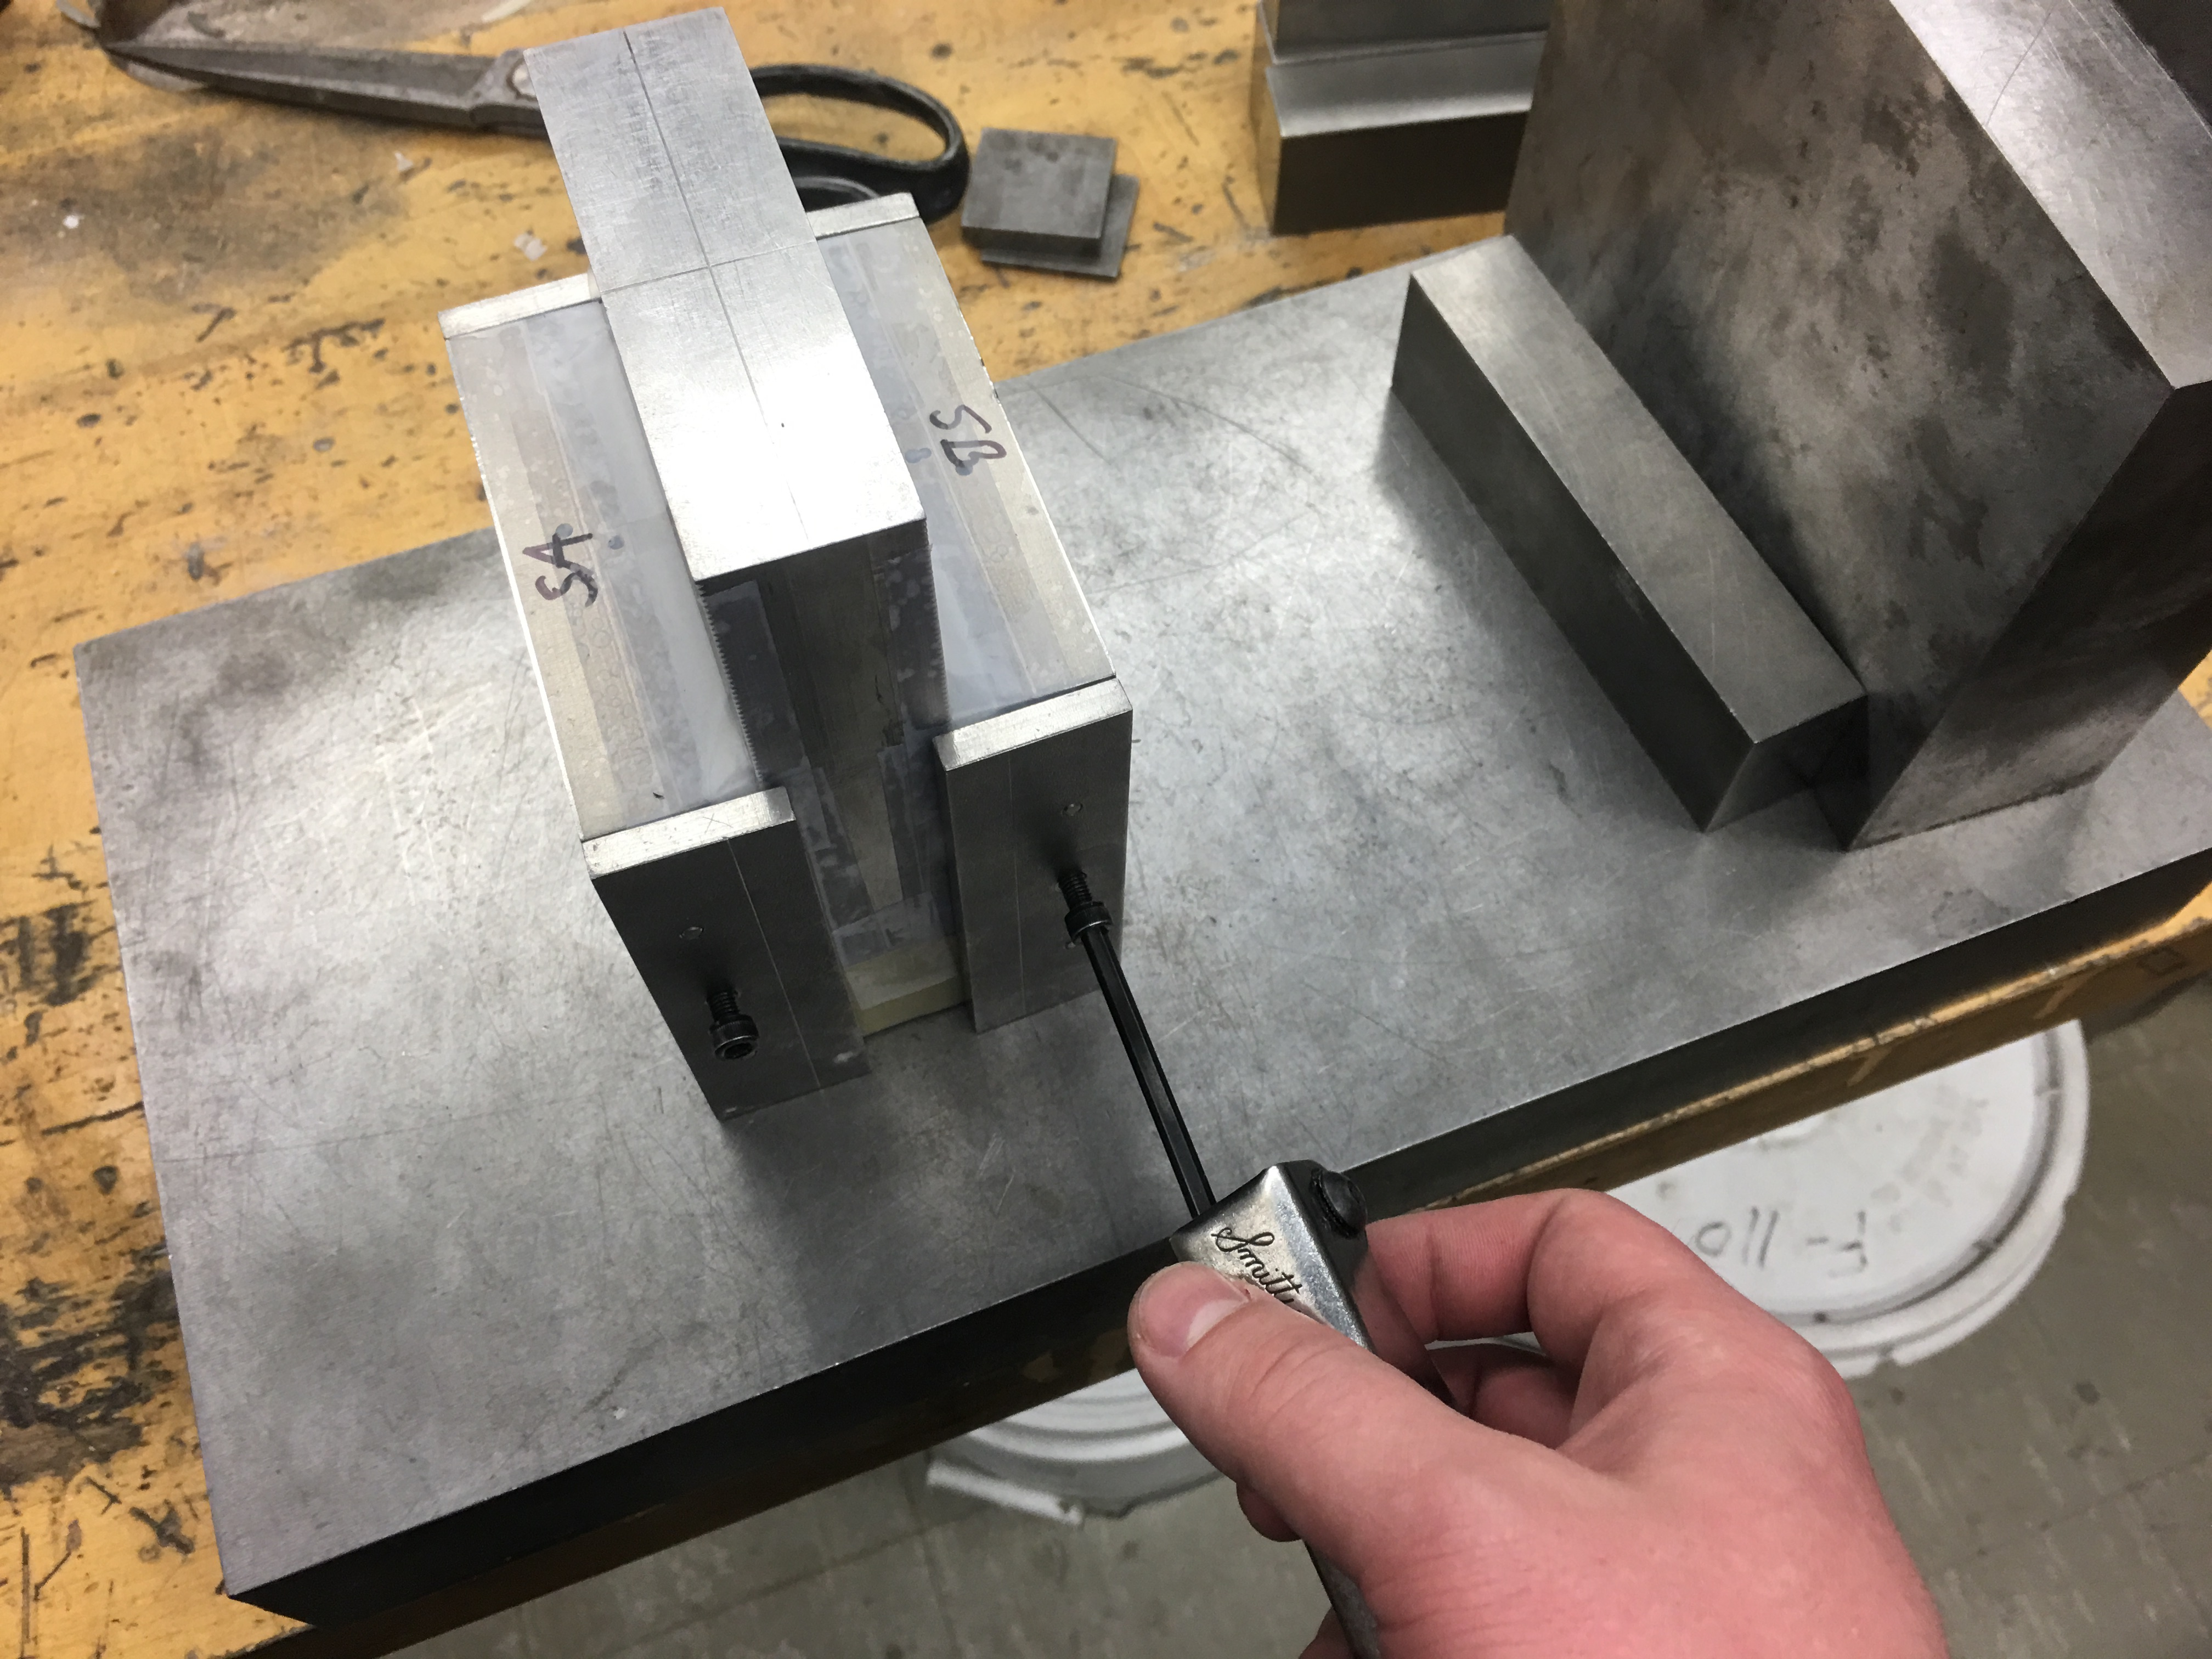
\includegraphics[width=0.7\textwidth]{appendix_sample_prep/dds_side_shields.jpg}
   	\caption{Secure the side shields to the sample assembly with the proper hardware. Replace any worn or stripped hardware.}
  	\label{Fig:dds_side_shields}
\end{figure}
%% End Figure %%

%% Figure %%
\begin{figure}
	\centering
        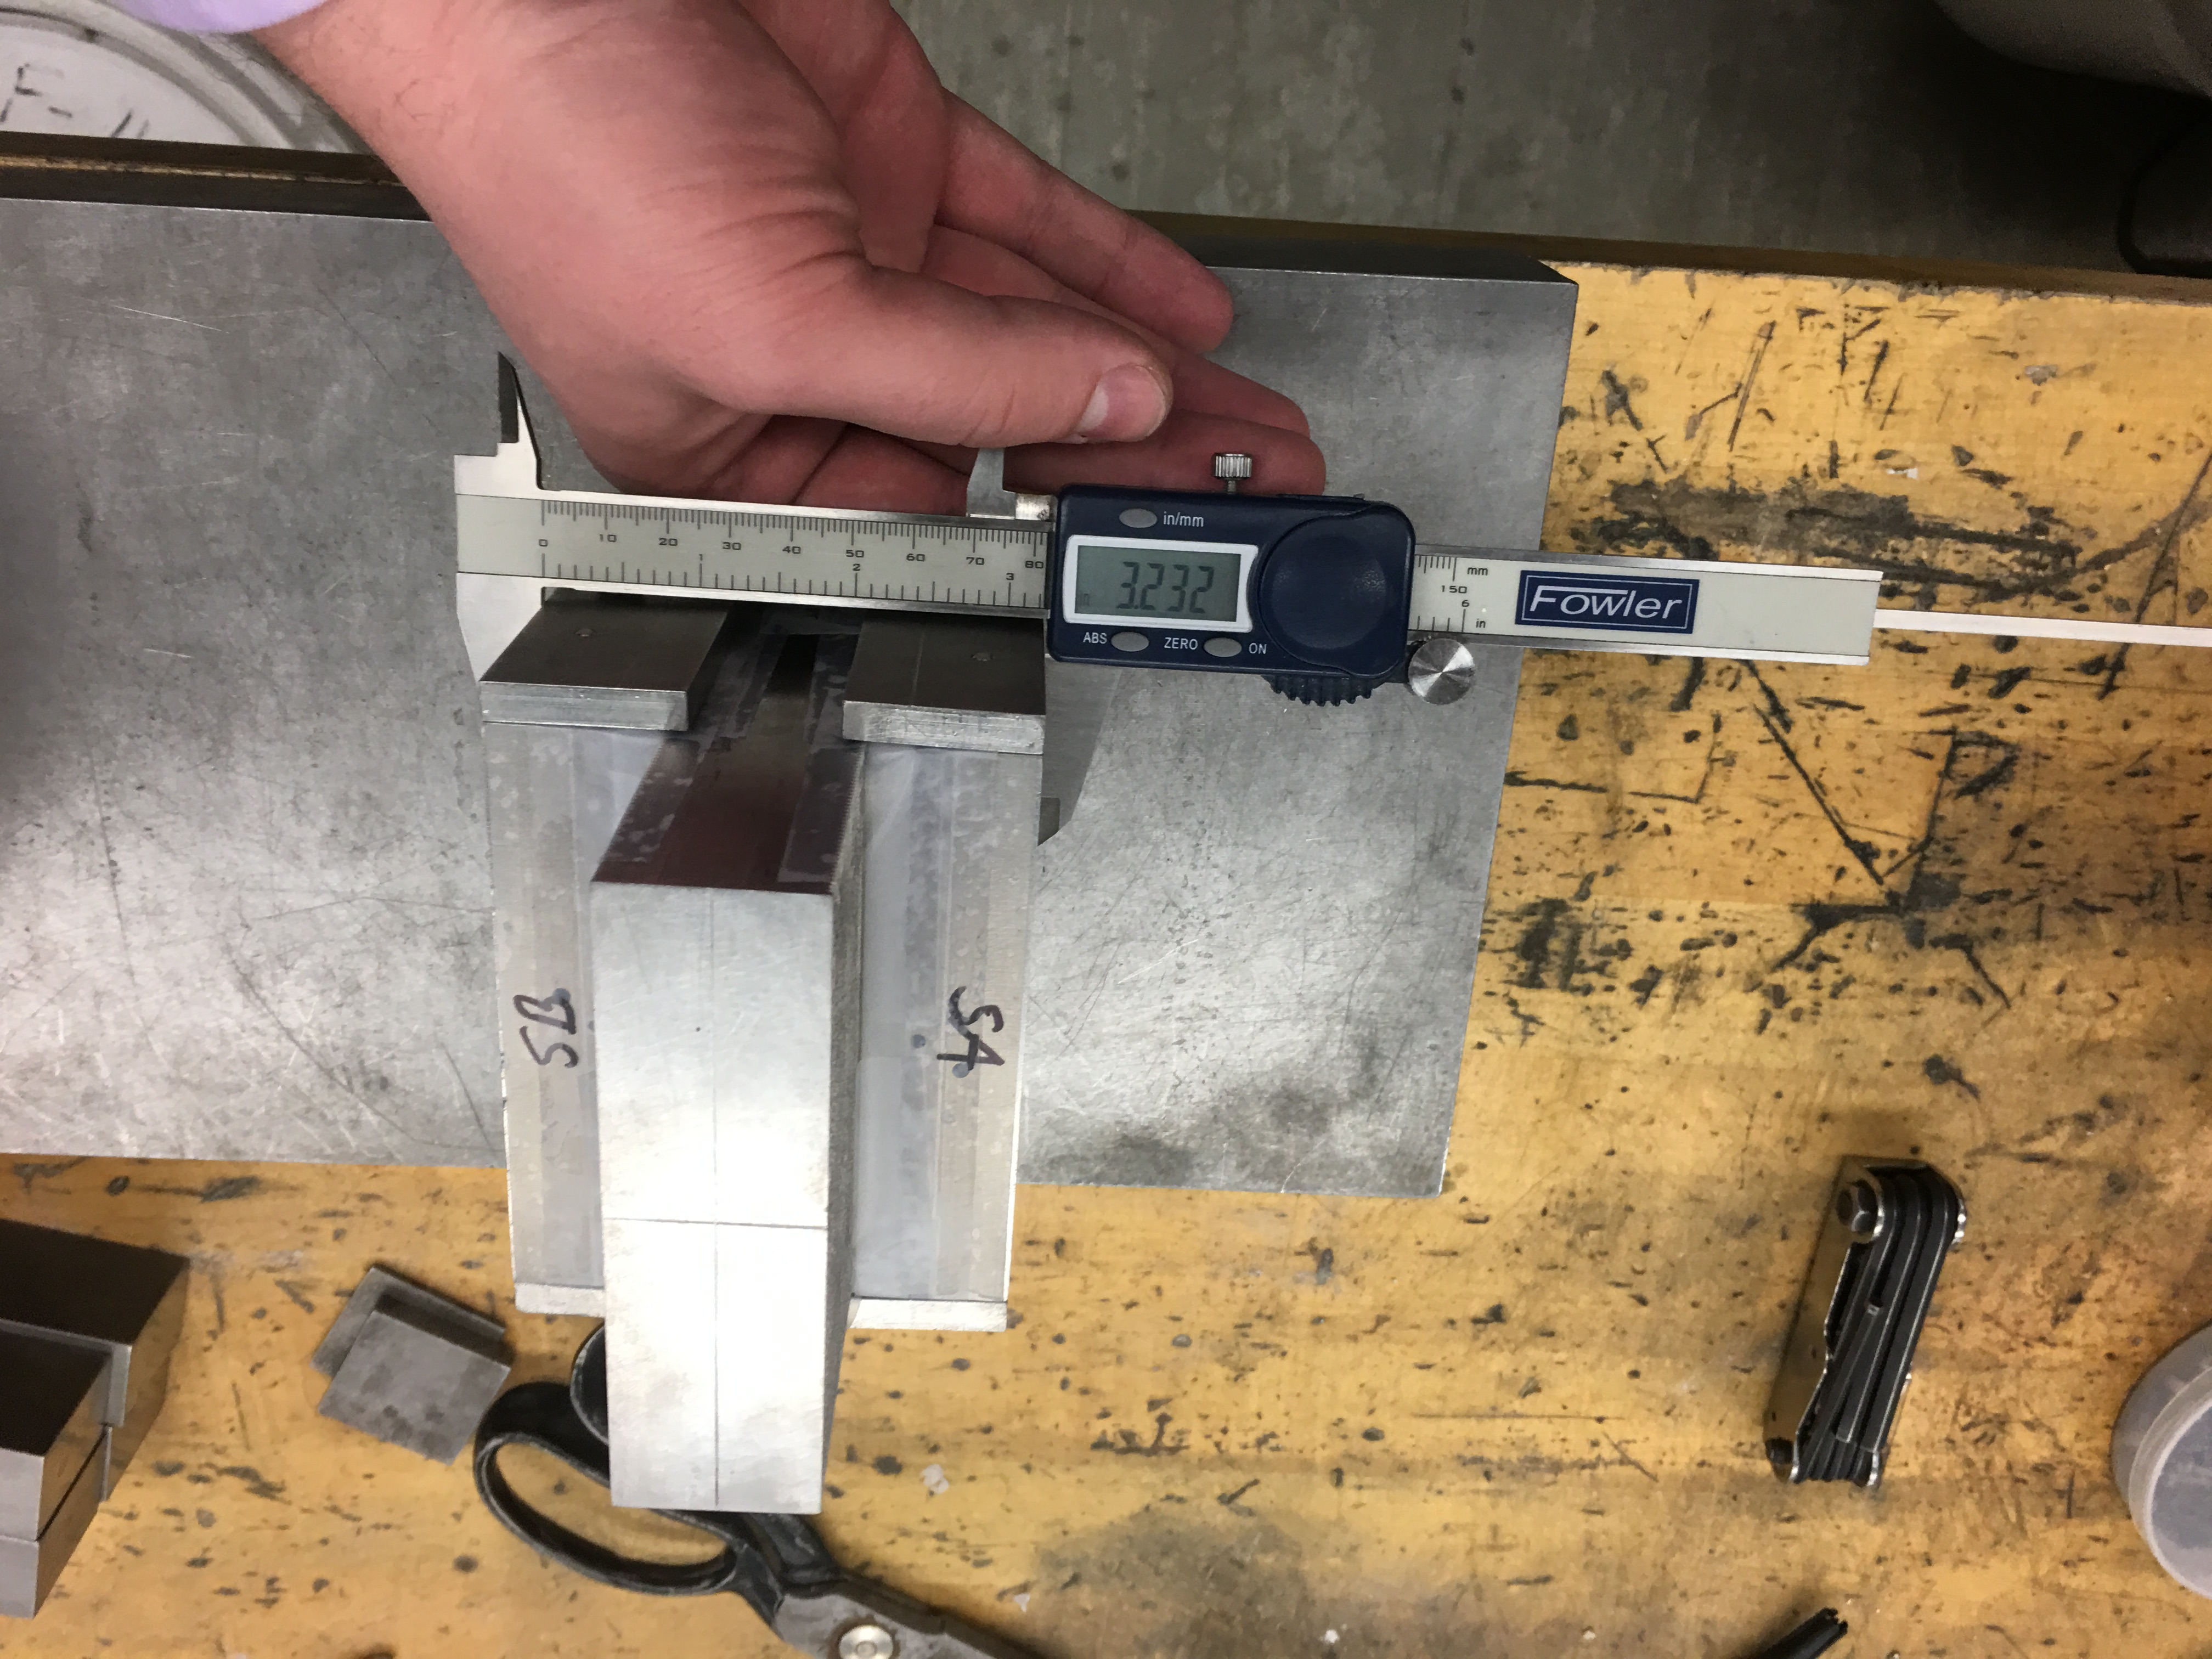
\includegraphics[width=0.7\textwidth]{appendix_sample_prep/dds_measure_sample.jpg}
   	\caption{Measure the bench thickness of the assembly using calipers and note it on the experiment run sheet.}
  	\label{Fig:dds_measure_sample}
\end{figure}
%% End Figure %%

%% Figure %%
\begin{figure}
	\centering
        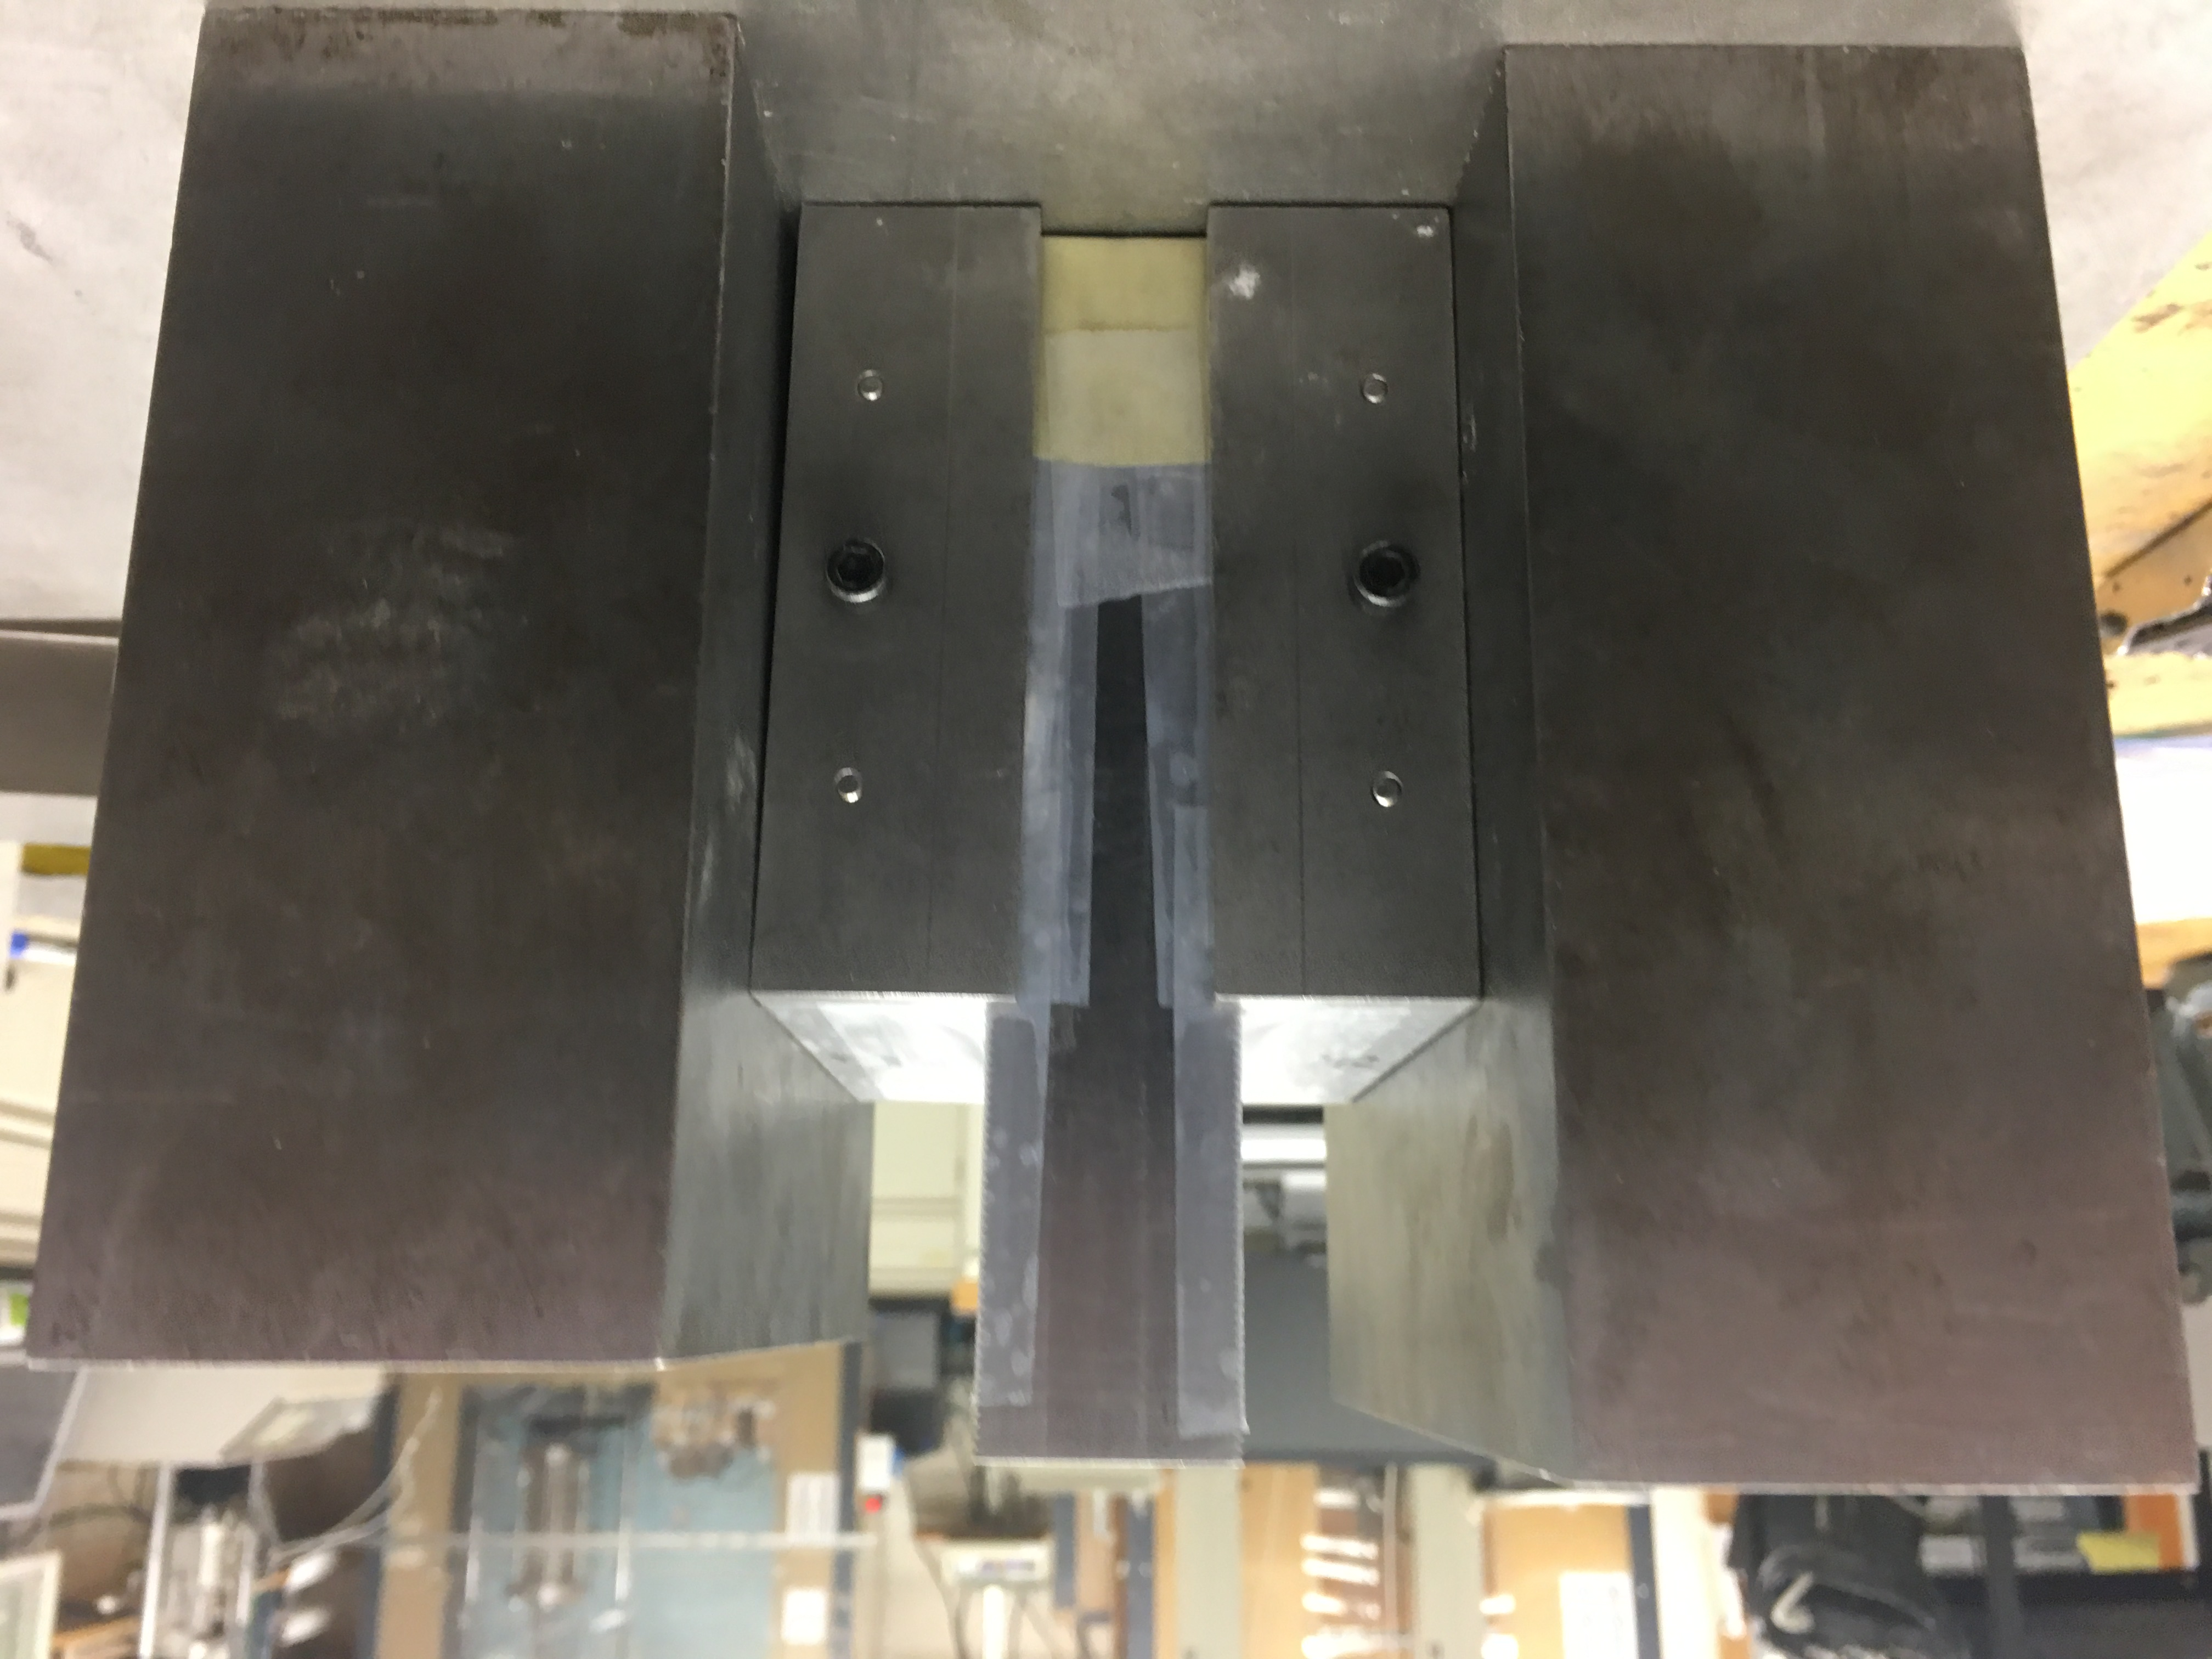
\includegraphics[width=0.7\textwidth]{appendix_sample_prep/dds_store_sample.jpg}
   	\caption{If the sample is not going to be run immediately, store it with slight pressure from two steel blocks to help prevent the layers from reshaping.}
  	\label{Fig:dds_store_sample}
\end{figure}
%% End Figure %%


\clearpage
\section{Triaxial Shrink Jacketing}
This section describes the process used to utilize shrink tube for jacketing rock and sediment samples in Temco pressure vessels.  Using shrink tube jackets allows the sample to be interrogated at very low confining pressures (the normal `black jackets' have a strength of $\sim$200 kPa).  We have successfully tested this method with no leaks on multiple samples.  There appears to be no side-flow even at confining pressures of just a few hundred kPa.  

\subsection{Materials}

\begin{itemize}

\item{(2) Black jacket sections}
\item{(1) Heat shrink tube}
\item{(1) Tie wire}
\item{(2) Frits}
\item{(3) Hose clamps}
\item{(1) Temco End caps and Piston Assembly}
\item{(1) Lineman's pliers}
\item{(1) Diagonal cutters}
\item{(1) Nutdriver for hose clamps}
\item{(1) Large flathead screwdriver}
\item{(1) Heat gun}
\item{(1) Scissors }


\end{itemize}

\subsection{Procedure}

\begin{enumerate}

\item{Prepare the sample plug as normal.  The regularity of the sides of the sample is slightly more forgiving than with the traditional setup.  Avoid any sharp surfaces that could puncture the jacket upon application of confining pressure.  A recommended length of 1" seems to be the best setup.}

\item{Cut a section of heat-shrink tube approximately 3-4" long.  This should cover the sample and most of the end-caps.}

\item{Ensure that the piston is retracted in the assembly.  Gently hammer down with a soft mallet if needed.  Watch out for oil being ejected during this process.}

\item{Place the short black jacket section over the piston and press most of the way down onto the shoulder, leaving a small gap of $\leq \frac{1}{4}$".}

\item{Place the bottom end-cap  and spacers in the Temco piston assembly and black jacket section.  Ensure there is solid metal-to-metal contact between the end-cap and the spacers in the jacket.}

\item{Using the flathead screwdriver, move the black jacket up until it will seal on the end cap and piston assembly suitably.}

\item{Secure the black jacket to the piston assembly with a hose clamp.  Tighten with the nut driver until snug.}

\item{Place the bottom porous frit, sample, and top porous frit on the assembly in that order.}

\item{Cover the sample assembly with the shrink tube.}

\item{Insert the top end-cap and align the column.}

\item {Ensure that the shrink tube covers the wire grooves on the end caps and does not cover the black jacket.}

\item{Holding the shrink tube in place, begin to heat it with the heat gun.  Work the heat gun from the bottom to the top of the sample.  Once the shrink tube will no longer slide down, begin the final shrinking.  Work up from the bottom of the sample, keeping the heat gun in constant motion.  This helps avoid any pockets forming between the sample and jacket.  The tube will not make a solid mechanical connection, this is normal.}

\item{After the shrink tube has been fixed, cut two 12-16" lengths of tie-wire.}

\item{Wrap the tie-wire over the shrink tube in the tie-wire retaining groove on the bottom end-cap.  Keep tension on the wire and pass it around the end-cap twice.  Place a few twists to hold the wire.  Be careful to not overlap the tie-wire!}

\item{Using a pair of pliers, grab the tie-wire at the base, pull to tighten, and rotate.  Repeat this process several times to fully seal the joint.  If the wire breaks, it was too tight.  This part requires some practice to ensure the proper tension.}

\item{Repeat the wire sealing procedure on the top end cap.  Be careful to not exert too much stress on the sample when doing this.}

\item{Trim excess tie wire to be $\sim \frac{1}{4}$" long.}

\item{Using a razor blade, trim away the excess shrink tube such that about  $\sim \frac{1}{8}$" is present behind the tie wire seal.  This metal surface area is necessary to ensure sealing of the black jacket and integrity of the shrink tube.}

\item{Seal the black jacket onto the bottom end-cap with a hose clamp.}

\item{Place the second black jacket segment onto the top end-cap.}

\item{Check the height of the column as compared to a normal, full length, black jacket.  These should be within  $\sim \frac{1}{8}$" of each other for proper sealing.  Sample length and black jacket segment length both modify this spacing.  Cut new black jacket segments to form the proper length assembly if necessary.}

\item{Clamp the black jacket segment onto the top end-cap with a hose clamp.}

\item{The sample is complete.  The Temco pressure cell can be loaded as normal.}

\end{enumerate}

%% Figure %%
\begin{figure}
	\centering
        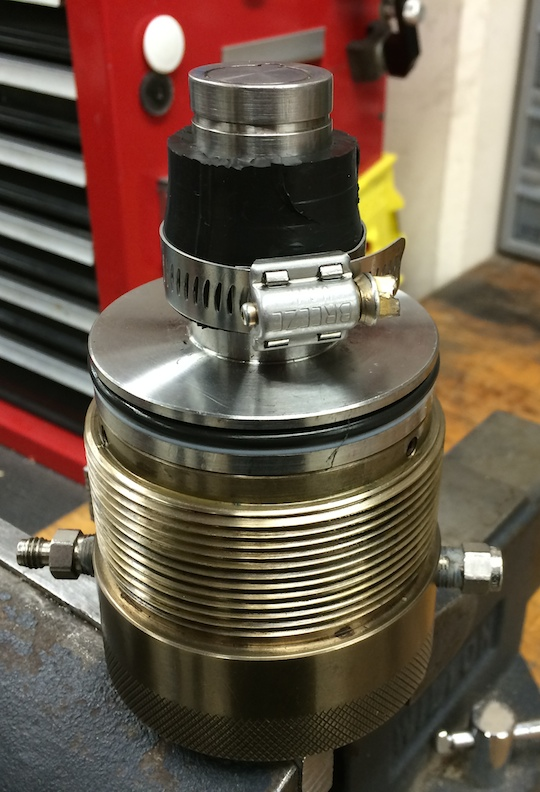
\includegraphics[scale=0.7]{appendix_sample_prep/piston_seal.jpg}
   	\caption{The black jacket section used to seal to the bottom piston assembly.  This jacket is as high as is acceptable.  It is recommended to start much lower and raise the jacket later to clamp it into place.}
  	\label{piston_seal}
\end{figure}
%% End Figure %%

%% Figure %%
\begin{figure}
	\centering
        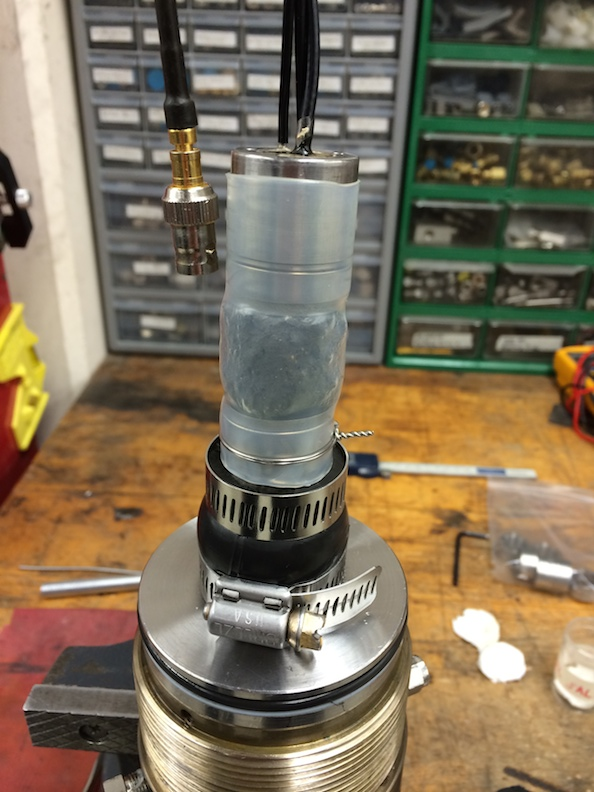
\includegraphics[scale=0.7]{appendix_sample_prep/after_shrink.jpg}
   	\caption{The sample after shrink tube is applied with a heat gun and the bottom tie wire is fixed.  Notice that there are no pockets or wrinkles in the jacket and it conforms smoothly to the sample surface.}
  	\label{after_shrink}
\end{figure}
%% End Figure %%

%% Figure %%
\begin{figure}
	\centering
        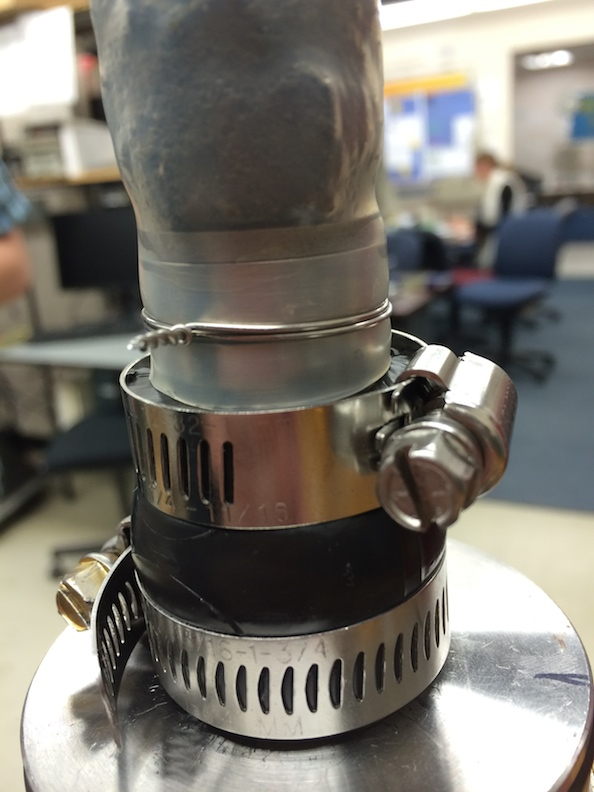
\includegraphics[scale=0.7]{appendix_sample_prep/seal_detail.jpg}
   	\caption{The piston end of the sample completely assembled.  The shrink jacket does not go inside the black jacket, but just to the top of it.  Hose clamps are used for additional insurance against leaks.  Care must be taken to avoid damaging the heat shrink or black jacket with sharp edges on the clamps.}
  	\label{seal_detail}
\end{figure}
%% End Figure %%

%% Figure %%
\begin{figure}
	\centering
        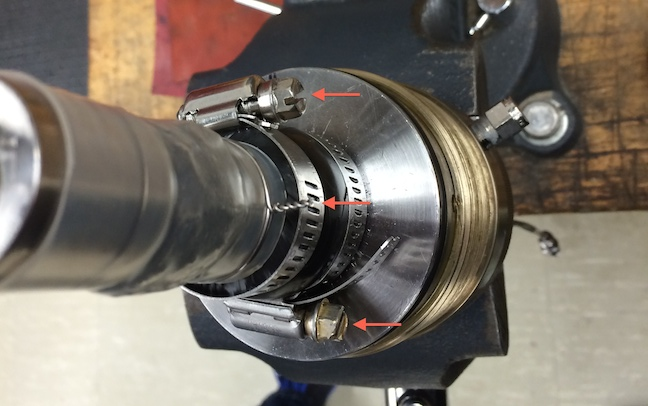
\includegraphics[scale=0.7]{appendix_sample_prep/seal_orientation.jpg}
   	\caption{To offset weak points in the sealing system, make sure that all clamp and tie points are offset by a minimum of 90$^\circ$.}
  	\label{seal_orientation}
\end{figure}
%% End Figure %%

%% Figure %%
\begin{figure}
	\centering
        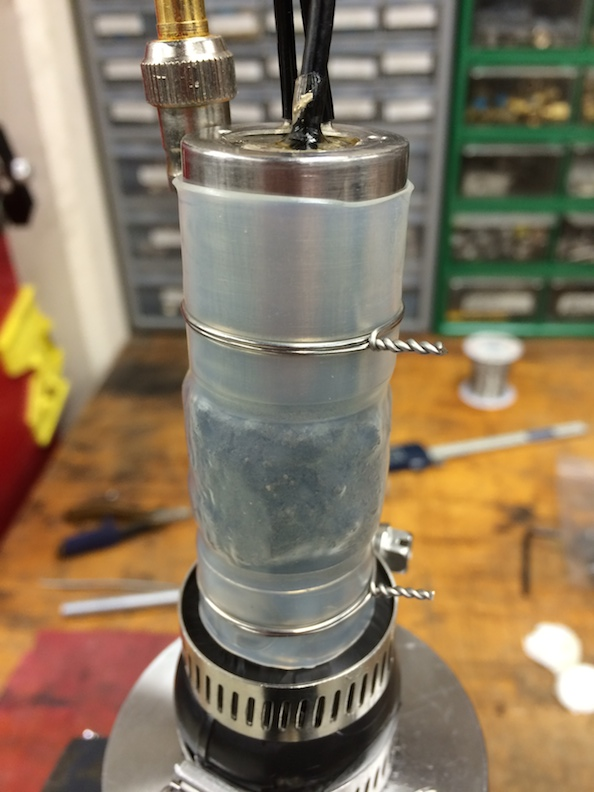
\includegraphics[scale=0.7]{appendix_sample_prep/all_tied.jpg}
   	\caption{Both tie wires have been affixed.  The wire does not overlap anywhere and sits on the groove in the end caps. Ends of the wire have been trimmed to  $\sim \frac{1}{4}$".}
  	\label{all_tied}
\end{figure}
%% End Figure %%

%% Figure %%
\begin{figure}
	\centering
        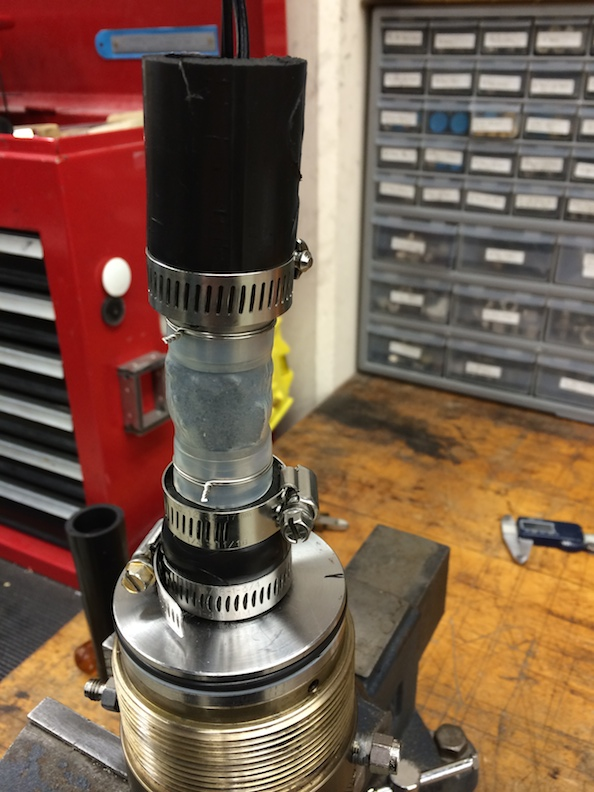
\includegraphics[scale=0.7]{appendix_sample_prep/final_stack.jpg}
   	\caption{The complete sample assembly, ready to be loaded into the pressure vessel and tested.}
  	\label{final_stack}
\end{figure}
%% End Figure %%
